\documentclass[a4paper,12pt]{article}
\usepackage[margin=25mm]{geometry}
\usepackage{amsmath}
\usepackage{amsfonts}
\usepackage{amssymb}
\usepackage{setspace}
\usepackage{fancyhdr,natbib}
\pagenumbering{arabic}  
\pagestyle{plain}
\usepackage{multirow}
\usepackage{multicol}
\usepackage{booktabs}
\usepackage{hyperref}
\usepackage{subcaption}
\usepackage{placeins}
\usepackage{textgreek}
\usepackage{graphicx}
\pagenumbering{gobble}
\usepackage{libertinus}
\usepackage[scaled=0.83]{courier}
\usepackage[T1]{fontenc}
\usepackage[utf8]{inputenc}
\usepackage{latexsym}
\renewcommand{\UrlFont}{\ttfamily\small}
\usepackage{verbatim}
\usepackage{gb4e}


\title{Acquiring Pronoun Cases: \\Insights from Pronoun Case Errors}
\author{Xiaomeng Ma }
\date{}
\begin{document}
\pagestyle{plain}
\pagenumbering{arabic}
\maketitle
\section{Introduction}
English-speaking children make pronoun case errors from the age of two to four. Some common types of errors include: (1) using an accusative pronoun (e.g. \textit{me, him, us}) or a genitive pronoun (e.g. \textit{my, his, our}) as the subject of the sentence, see (\ref{1}) and (\ref{3}); (2) using a nominative pronoun (e.g. \textit{I, she, he}) or a genitive pronoun as the object in a sentence, see (\ref{2}) and (\ref{4}) and (3) using an accusative pronoun as the determiner, see (\ref{5}) and (\ref{6}). Researchers have categorized such errors as systematic, characteristic and frequent \citep[e.g.][]{huxley1970development, budwig1989linguistic, pelham2011input,fitzgerald2017case}.

\begin{exe}
\ex \label{01} non-nominative subject:
\begin{xlist}
\ex \label{1} {Where does \textit{him} go? - \textit{him} for \textit{he}, Becky at the age of 2;6\footnote{\href{https://childes.talkbank.org/browser/index.php?url=Eng-UK/Manchester/Becky/020619.cha}{Manchester/Becky/020619.cha}
}}
\ex \label{3} {\textit{My} get my car. - \textit{my} for \textit{I}, Nina at the age of 2;0\footnote{\href{https://childes.talkbank.org/browser/index.php?url=Eng-NA/Suppes/020003.cha}{Suppes/020003.cha}}}
\end{xlist}
\ex non-accusative object:
\begin{xlist}
\ex \label{2} {Mama put \textit{he} here. - \textit{he} for \textit{him}, Tow at the age of 1;9\footnote{\href{https://childes.talkbank.org/browser/index.php?url=Eng-NA/Post/Tow/010909.cha}{Post/Tow/010909.cha}}}
\ex \label{4} {Watch \textit{my} going round, Mum. - \textit{my} for \textit{me}, Gail at the age of 2;4\footnote{\href{https://childes.talkbank.org/browser/index.php?url=Eng-UK/Manchester/Gail/020421.cha}{Manchester/Gail/020421.cha}}}
\end{xlist}
\ex non-genitive determiner:
\begin{xlist}
\ex \label{5} He doesn't have \textit{them} claws. -\textit{them} for \textit{those/these} Roman at the age of 3;5\footnote{\href{https://childes.talkbank.org/browser/index.php?url=Eng-NA/Weist/Roman/030501.cha}{Weist/Roman/030501.cha}}
\ex \label{6} Um and that's \textit{me} name. - Fraser at the age of 3;0\footnote{\href{https://childes.talkbank.org/browser/index.php?url=Eng-UK/MPI-EVA-Manchester/Fraser/030025a.cha}{MPI-EVA-Manchester/Fraser/030025a.cha}}
\end{xlist}
\end{exe}

The most well-studied error is the non-nominative subject, where an accusative pronoun or a genitive pronoun is used in the subject position, as shown in (\ref{01}). Theoretically, the nominative case is licensed by the +\textsc{finite} feature on the IP. If the +\textsc{finite} is missing, the nominative case won't be checked. Therefore, the syntactic explanation linked this error with children's use of finite verbs \citep[e.g.][]{vainikka1993case,wexler1996, schutze1996subject}. Young children often go through a period in language development when they sometimes omit inflections on the verbs, producing non-finite forms such as `Then the horse \textit{jump}.' This developmental stage referred to by \cite{wexler1994,wexler1998,wexler2000} as the `Optional Infinitive Stage', where finiteness is optional in children's grammar, even though they already have the syntactic knowledge of tense and agreement. When the children produce a non-finite verb by omitting the inflections, the nominative case are not checked, leading to the non-nominative subject errors, such as `Then \textit{him/his} jump'. In the syntactic explanation, the non-nominative subject stems from children's problematic use of finite verbs and it is characteristic at Optional Infinitive Stage.

Although the syntactic explanation can account for many observed error patterns, not all the predictions are correct. According to the syntactic explanation, when a non-nominative subject is present, the verb in that sentence is unlikely to be a finite verb. \cite{pine2005testing} found that the data doesn't always support this prediction since it is not uncommon for children to produce non-nominative subjects with finite verbs. 

In addition, the syntactic explanation doesn't address the questions of individual variations, such as why different children make errors with different forms. For example, in example (\ref{1}), Becky replaced the nominative pronoun \textit{he} with its accusative form \textit{him}; whereas Nina replaced the nominative pronoun \textit{I} with the its genitive form \textit{my} in (\ref{3}). Meanwhile, \textit{my} was used as a substitute for the accusative pronoun \textit{me} by Gail in (\ref{4}).  \cite{rispoli1998} studied non-nominative use of pronoun \textit{I} and found that the majority of the children predominantly make `\textit{me}-for-\textit{I}' error and a minority predominantly make `\textit{my}-for-\textit{I}' error. He then found that the `\textit{me}-for-\textit{I}' is highly correlated with the correct use of `\textit{me}' in children's production. Thus, \cite{rispoli1998,rispoli1999,rispoli2005} treated pronoun case error as lexical retrieval error that is closely related with children's pronominal use. He proposed that for each pronoun, case, person, and number form a 3x3 paradigm. Young children have difficulties accessing all forms of pronouns in the paradigm, and thus make pronoun errors. 




In addition, parents' input also could play an important role in pronoun errors. \cite{pelham2011input} suggests that English children make more pronoun case errors than German children because English has more case-ambiguous pronouns (e.g. \textit{you}, \textit{it} and \textit{her}) than German. Parents' input also contains many ambiguous phrases like `Let \underline{\textit{me} do it}' or `help \underline{\textit{her} open it}' that could potentially confuse the children, that they would produce erroneous utterances such as `\underline{\textit{me} do it}' or `\underline{\textit{her} open it}' \citep{tomasello2000, kirjavainen2009can}.  




Apart from non-nominative subjects, children also substitute the accusative case for genitive case, as in (4) and substitute genitive case for an accusative case, as in (5). These errors have been generally overlooked by previous studies.
\begin{exe}
\ex [*]{Don't take \textit{me} bottle out. - \textit{me} for \textit{my}, Nina at the age of 2;1\footnote{\href{https://childes.talkbank.org/browser/index.php?url=Eng-NA/Suppes/020115.cha}{Suppes/020115.cha}}}
\ex [*]{Let \textit{my} try. - \textit{my} for \textit{me}, Carl at the age of 2;6\footnote{\href{https://childes.talkbank.org/browser/index.php?url=Eng-UK/Manchester/Carl/020619.cha}{Manchester/Carl/020619.cha}} }
\end{exe}
The existing explanations seem to fall short for these errors. The syntactic explanations treat the accusative case and the genitive case as two different default forms to the nominative case. If both cases are default, there is no incentive to substitute one default for the other as in (4) and (5). Moreover, parents' input never contain any segments that resemble the errors in (4) and (5): `take \textit{me} bottle' and `let \textit{my} try'. 

Moreover, after over 40 years of research, some basic properties of pronoun case errors are still unknown, such as the frequencies and distributions of the errors, at what age are those errors likely to occur, how prevalent are those errors among children, does the error disappear after the children reach a certain age or a certain MLU, etc. Few studies have reported comprehensive pronoun error counts or error rates; instead, most of the studies focused on a certain type of errors or pronouns in their analysis. A sizable longitudinal dataset is required to answer these questions. One common limitation for previous studies is their small sample size: \cite{schutze1996subject} included 3 children (Nina from \citep{suppes1974semantics}, Sarah from \citep{brown1973first} and Peter\citep{bloom1974imitation}); \cite{rispoli1998} collected data on 12 children from 1;0 to 3;0; \cite{kirjavainen2009can} conducted corpus analysis of 17 children in CHILDES (12 from Manchester corpus \cite{theakston2001}, Fraser and Eleanor from densed corpus \citep{rowland2006effect} and Abe from \cite{kuczaj1977acquisition}, Nina from \citep{suppes1974semantics} and Peter from \citep{bloom1974imitation}). Due to limited sample size, previous studies couldn't address these questions. 

This paper investigated pronoun case errors in children's production by conducting a comprehensive corpus analysis on all the available data of English-speaking children on \textsc{childes} \citep{macwhinney2014childes}. First, this paper reviewed some basic features of pronoun case errors, such as frequency and distribution, age range, correlation with age and MLU, etc. Second, this paper re-examined each existing explanations using all available CHILDES data. In the previous studies, researchers either collected their own data or used different corpora to test their hypotheses. It is necessary to evaluate different theories on the same set of data in order to control for collection bias or limitations of small sample size. 

Last, this paper will provide a hypothesis about how children acquire pronoun case in the first place. Cases are used to mark different relationship between arguments, which is a more abstract grammatical feature to learn compared to plural forms or tense marking. Yet young children are able to produce the correct form of a pronoun in different argument positions. It would be worthwhile to ask the question: how do children acquire this abstract feature at such a young age? This study is going to test two hypotheses of the acquisition of pronoun case. From a theoretical perspective, the children could derive different cases through argument structure. Nominative case and accusative case could be differentiated at the sentential level, such that the former is associated with the subject and the latter case is associated with the object. In addition, children could also acquire cases through statistical learning. Nominative case, accusative case and genitive case have different distributional patterns in speech, which difference could be utilized by children to acquire different cases. 

The paper is organized as follows: Section 2 presents a detailed description of pronoun case errors, including the basic properties metioned above; Section 3 - 5 replicates representative studies for existing explanations and evaluates that explanation; Section 6 demonstrates a computational model using distributional patterns to explain pronoun case acquisition.
\newpage
\section{The Basic Features of Pronoun Case Error}
\subsection{Corpora}
To avoid the limitation of small sample size and data selection bias, this study conducted a comprehensive corpus analysis of speech from monolingual English-speaking children from roughly ages two to four. That includes 46 children with longitudinal recordings in CHILDES. Table \ref{table:1} shows the summary of the corpus.

\begin{table}[h]
\footnotesize
\centering
\caption{Summary of Corpus Information} 
\label{table:1}
%\begin{adjustbox}
\begin{tabular}{l|l|l|l|l|l}
\toprule
\multicolumn{6}{c}{\textbf{North American Corpora}} &
\hline
\textbf{Corpora}  & \textbf{Child}  & \textbf{Age} &
\textbf{Corpora}  & \textbf{Child}  & \textbf{Age}\\
\hline
\cite{bloom1974imitation}  & Peter   & 1;9-3;2 & \cite{suppes1974semantics} &  Nina & 2;0-3;4
\\
\cite{braunwald1971mother}  & Laura   & 1;5-4;0 & \cite{kuczaj1978children} &  Abe & 2;5-4;0 \\
\multirow{}{}*{\cite{brown1973first}} & Adam & 2;3-4;0 & \cite{demetras1986working} & Trevor & 2;1-4;0\\
& Eve & 1;6-2;3 & \multirow{}{}*{\cite{Weist2009}} & Ben & 2;4-3;4 \\
& Sarah & 2;3-4;0 & &Emily & 2;6-3;4\\
\cite{demetras1989changes} & Jimmy & 2;2-2;10 & & Emma & 2;7-3;9\\
\cite{clark1978awareness} & Shem & 2;3-3;2 &  & Jilian & 2;1-2;10\\
\cite{sachs1983talking}& Naomi & 1;3-4;9 & & Matt & 2;5-5;0\\
\cite{macwhinney2014childes} & Ross & 1;4-5;0 & & Roman & 2;3-4;0\\
\multirow{}{}*{\cite{post1993language}}& She & 1;8-2;5 & \cite{Snow1990child} & Nathaniel & 3;1-3;3\\
&Tow&1;9-2;5&\cite{hayes1988vocabulary}&Geraldine&1;6-2;2\\
\hline
\hline
& \textbf{No.} & \textbf{Mean Age} & & \textbf{No.} & \textbf{Mean Age}\\
\cite{bates1991first}  & 11  & 2;4 &
\cite{bohannon1977children}  & 2 & 3;6\\
\cite{gleason1980acquisition}&19&4;8&\cite{snow1995shell}&79&3;11\\
\cite{snow1989imitativeness}&25&2;8&\cite{valian1991syntactic}&17&2;5\\
\cite{van1980effects}&19&3;9\\
\hline
\hline
\multicolumn{6}{c}{\textbf{UK Corpora}}&
\hline
\textbf{Corpora}  & \textbf{Child}  & \textbf{Age} &
\textbf{Corpora}  & \textbf{Child}  & \textbf{Age}\\
\hline
\multirow{}{}*{\cite{henry1995belfast}} & Barbara & 2;4-4;1 & \multirow{}{}*{\cite{theakston2001}} & Anne & 1;10-2;9\\
& Michelle & 2;4-4;4 & & Warren& 1;10-2;9 \\
& Courtney & 3;4-4;0 & &Aran & 1;11-2;10\\
 & Rachel & 2;5-3;2 & & Becky & 2;0-2;11\\
 & Conor & 3;8-4;5 &  & Carl & 1;8-2;8\\
& Stuart & 3;5-4;5 & & Dominic & 1;10-2;10\\
 & Johnny & 3;5-4;4 & & Gail & 1;11-2;11\\
 & David & 2;0-4;2 &  & Joel & 1;11-2;10\\
\cite{rowland2006effect} & Lara & 1;9-3;3&  & John &1;11-2;10 \\
\cite{maslen2004dense} & Thomas & 2;0-4;11 & & Liz& 1;11-2;10\\
\multirow{}{}*{\cite{lieven2009two}} &Eleanor &2;0-3;1 & & Nicole& 2;0-3;0 \\
&Fraser &2;0-3;0 & & Ruth& 1;11-2;11 \\
\hline
\hline
&\textbf{No.}&\textbf{Mean Age}& &\textbf{No.}&\textbf{Mean Age}\\
\cite{tommerdahl2013analyzing}&23&2;9&\cite{howe1981acquiring}&16&2;0\\
\hline
\bottomrule
\end{tabular}
%\end{adjustbox}
\end{table}

This study applied the \textsc{nltk} python package to automatically extract data from the annotated corpora in CHILDES. The data that has been collected from each child's file include their age, mlu, total number of children's words and parents' words, total number of children's sentences and parents' sentences, total number of each pronoun produced by the children and produced by the parents. 

\subsection{Finding Errors}
The annotated \texttt{.xml} files were used to search for the errors. CHILDES applies MOR and GRASP programs to annotate part-of-speech tags and dependency grammatical relations for all the transcripts. For English data, the automated annotation system has been reported to have high-level accuracies: the MOR program reaches 97\% of accuracy and the GRASP program has 95.8\% accuracy for identifying the subjects and 94.1\% accuracy for identifying the objects \citep{macwhinney2012morphosyntactic,sagae2010morphosyntactic}. The MOR program produces the \texttt{\%mor} tier, in which part-of-speech tags stand in one-to-one correspondence with the word in the transcript line. The \texttt{\%mor} tier assigns \texttt{pro:sub} to the nominative pronouns, \texttt{pro:obj} to the accusative pronouns and \texttt{det:poss} to the genitive pronouns. Case-ambiguous pronouns `you' and `it' are tagged as \texttt{pro:per} which doesn't differentiate their nominative use and accusative use. Pronoun `her' is tagged as \texttt{pro:obj} when it is used as an object and \texttt{det:poss} when it is used as a determiner. The GRASP program produces the \texttt{\%gra} tier which represents grammatical relations. The \texttt{\%gra} assigns \texttt{SUBJ} for the word in the subject position,  \texttt{OBJ} or \texttt{POBJ} for the word in the object position, and \texttt{DET} for the word in the determiner position. The \texttt{\%mor} tier assigns the case (e.g. \texttt{pro:sub} or \texttt{pro:obj}) based on the pronoun itself, regardless of the context it is used in. The \texttt{\%gra} tier assigns the case based on the argument position, despite the pronoun's own case. An excerpt from Peter in the Brown corpus in (\ref{example}) exemplifies the \texttt{\%mor} tier and \texttt{\%gra} tier. All the errors were first extracted using the \texttt{nltk} python package \citep{bird2009natural}, and then hand-checked by two annotators independently. 
\begin{exe}
\ex \label{example} \gll *CHI: \textbf{you}'re getting vitamins for \textbf{me }.\\
\%mor:	\textbf{pro:per|you}~aux|be&PRES part|get-PRESP n|vitamin-PL prep|for \textbf{pro:obj|me} .\\
\%gra:\textbf{	1|3|SUBJ} 2|3|AUX 3|0|ROOT 4|3|OBJ 5|3|JCT \textbf{6|5|POBJ} 7|3|PUNCT\\
(\href{https://childes.talkbank.org/browser/index.php?url=Eng-NA/Bloom/Peter/020812.cha}{Bloom/Peter/020812.cha})
\end{exe}

\subsubsection{NOM case errors and ACC case errors}
The NOM case errors are the nominative cased pronouns used in the non-subject position, e.g. `she hit \textit{I}'. The ACC case errors are the accusative cased pronouns used in the non-object position, e.g. `\textit{me} drink milk'. These two types of errors were located on \texttt{\%gra} tier, since \texttt{\%gra} tier identifies subject and object based on the the relationship between arguments. For nominative cased pronouns \textit{I, he, she, we, they}, if they appear in a sentence with dependency grammatical relations \footnote{Children produce many incomplete sentences and run-on sentences. Not all the incomplete sentences have dependency grammatical relations, such as \textit{`I yeah'} and \textit{`um I I I.'}. To have dependency grammatical relations, the sentence needs to have at least two words from different grammatical categories that can be combined together. Sentences without dependency grammatical relations are excluded in this study.} 
and if they are not tagged as \texttt{SUBJ} on the \texttt{\%gra} tier, it is counted as an error. For example, in sentence (\ref{meseehe}), the nominative cased pronoun \textit{`he'} is used in an object position and it is tagged as \texttt{OBJ} on the \texttt{\%gra} tier. In (\ref{hehat}), \textit{`they'} is tagged as \texttt{POBJ} (object) on the \texttt{\%gra} tier too. 
\begin{exe}
\ex \label{meseehe}\gll *CHI: when \textit{\textbf{me}} see \textit{\textbf{he}} again ?\\
\%mor: conj|when \textit{\textbf{pro:obj|me}} v|see \textit{\textbf{pro:sub|he}} adv|again ? \\
\%gra: 1|3|LINK \textbf{\textit{2|3|SUBJ}} 3|0|ROOT \textit{\textbf{4|3|OBJ}} 5|4|JCT 6|3|PUNCT \\
(\href{https://childes.talkbank.org/browser/index.php?url=Eng-NA/Brown/Eve/020100b.cha}{Brown/Eve/020100b.cha})
\ex \label{hehat}\gll *CHI: all of \textit{\textbf{they}} going go in here.\\
\%mor: pro:indef|all prep|of pro:sub|they part|go-PRESP~inf|to v|go prep|in n|here\\
\%gra: 1|0|INCROOT 2|1|NJCT 3|2|POBJ 4|3|XMOD 5|6|INF 6|4|COMP 7|6|JCT 8|7|POBJ 9|1|PUNCT.\\
(\href{https://childes.talkbank.org/browser/index.php?url=Eng-NA/Suppes/021021.cha}{Suppes/021021.cha})
\end{exe}
Similar to the searching process for the NOM case errors, for accusative cased pronouns \textit{me, him, us, them}, if they appear in a sentence with dependency grammatical relations and if they are not tagged as \texttt{OBJ} or \texttt{POBJ}, they were counted as errors. For example, in sentence (\ref{meseehe}) and (\ref{666}), \textit{me} is an accusative cased pronoun and it was used as the subject, which was tagged as \texttt{SUBJ}. In sentence (\ref{meshoew}), \textit{me} is used as a determiner, which was tagged as \texttt{MOD}(modifier). In sentence (\ref{them}), \textit{them} is used as a determiner, but it was tagged as \texttt{SUBJ} on the \texttt{\%gra} tier. Although the tag is not correct, as long as it is not tagged as \texttt{OBJ} or \texttt{POBJ}, it is still counted as an error. The third person singular feminine pronoun \textit{her} is a special case, because it can be used as an object or a determiner. The \texttt{\%mor} tier is used to distinguish accusative \textit{her} and genitive \textit{her}. The former is tagged as \texttt{pro:obj} and the latter is tagged as \texttt{det:poss}. All the \textit{her}s that are not tagged as \texttt{OBJ} or \texttt{POBJ} or \texttt{DET} or \texttt{MOD} on the \texttt{\%gra} tier are counted as error. For example, in (\ref{herdidnt}), \textit{her} is tagged as \texttt{SUBJ} on the \texttt{\%gra} tier, thus counted as an error. 

All the NOM and ACC errors were first identified using the \texttt{nltk} python package and hand checked by two annotators. 

\begin{exe}
\ex \label{666}\gll *CHI: \textit{\textbf{me}} come back.\\
\%mor: \textit{\textbf{pro:obj|me}} v|come adv|back .\\
\%gra: \textit{\textbf{1|2|SUBJ}} 2|0|ROOT 3|2|JCT 4|2|PUNCT. \\
(\href{https://childes.talkbank.org/browser/index.php?url=Eng-NA/Brown/Eve/011000a.cha}{Brown/Eve/011000a.cha})
\ex \label{meshoew} \gll *CHI:	where's \textbf{\textit{me}} shoes ?\\
\%mor:	pro:int|where~cop|be&3S \textit{\textbf{pro:obj|me}} n|shoe-PL ?\\
\%gra:	1|2|SUBJ 2|0|ROOT \textbf{\textit{3|4|MOD}} 4|2|PRED 5|2|PUNCT\\
(\href{https://childes.talkbank.org/browser/index.php?url=Eng-NA/Suppes/020228.cha}{Suppes/020228.cha})
\ex \label{them} \gll *CHI:	\textbf{\textit{them}} guys can beat up this guy .\\
\%mor:	\textit{\textbf{pro:obj|them}} n|guy-PL n|can n|beat adv|up det:dem|this n|guy .\\
\%gra:\textbf{\textit{	1|2|SUBJ} }2|4|MOD 3|4|MOD 4|0|ROOT 5|4|NJCT 6|7|DET 7|5|POBJ 8|4|PUNCT\\
(\href{https://childes.talkbank.org/browser/index.php?url=Eng-NA/Kuczaj/020700.cha}{Kuczaj/020700.cha})
\ex \label{herdidnt}\gll *CHI: \textit{\textbf{her}} didn't wanna.\\
\%mor: \textbf{\textit{det:poss|her}} mod|do&PAST~neg|not v|want~inf|to .\\
\%gra:	\textit{\textbf{1|4|SUBJ}} 2|4|AUX 3|2|NEG 4|0|ROOT 5|4|OBJ 6|4|PUNCT. \\
(\href{https://childes.talkbank.org/browser/index.php?url=Eng-NA/Brown/Eve/020300b.cha}{Brown/Eve/020300b.cha})
\end{exe}


\subsubsection{GEN case error}
Genitive case errors were not identified in the \texttt{\%gra} tier, since the \texttt{\%gra} tier is less successful in capturing phrasal relationships. The genitive cased pronouns are not always tagged as \texttt{SUBJ} or \texttt{OBJ} even when they appear in the subject or object position. For example in (\ref{mywantit}), the genitive case pronoun `\textit{my}' is in the subject position, but it is tagged as \texttt{DET} (determiner) on the \texttt{\%gra} tier. 

Instead, genitive case errors are located using \texttt{\%mor} tier by a search of all the impossible part-of-speech tag combinations that contain a determiner. Genitive cased pronouns could be mistakenly used as a subject or an object in the sentence. When a genitive cased pronoun is misused as a subject, it is likely to precede a verb; and when it is misused as an object, it is likely to appear after a verb. Therefore, when a genitive cased pronoun, \textit{my, his, our, their}, occurs with a verb, including past and present participles (in (\ref{got}) and (\ref{mywantit})) and auxiliaries (in (\ref{mycan}) and (\ref{his}), it is counted as an error. 

\begin{exe}
\ex \label{} \gll *CHI:	when \textit{\textbf{my}} take a nap. \\
\%mor:	conj|when \textit{\textbf{det:poss|my}} v|take det:art|a n|nap.\\
\%gra:	1|3|LINK 2|3|DET 3|0|ROOT 4|5|DET 5|3|OBJ 6|3|PUNCT.
\ex \label{got} \gll *CHI: yeah \textit{\textbf{my}} got.\\
\%mor: co|yeah \textit{\textbf{det:poss|my}} v|get&PAST.\\
\%gra: 1|3|COM \textit{\textbf{2|3|DET }} 3|0|ROOT.\\
(\href{https://childes.talkbank.org/browser/index.php?url=Eng-NA/Brown/Sarah/030018b.cha}{Brown/Sarah/030018b.cha})
\ex \label{mywantit} \gll  *CHI: what \textit{\textbf{my}}  doing?  \\     
\%mor:	pro:int|what \textit{\textbf{det:poss|my}} part|do-PRESP?\\
\%gra:	1|3|LINK \textit{\textbf{2|3|DET}} 3|0|ROOT 4|3|PUNCT\\
(\href{https://childes.talkbank.org/browser/index.php?url=Eng-NA/Brown/Eve/020100b.cha}{Brown/Eve/020100b.cha})
\ex \label{mycan} \gll *CHI: \textit{\textbf{my}} can sing.\\
\%mor: \textbf{\textit{det:poss|my}} mod|can v|sing.\\
\%gra: \textit{\textbf{1|3|DET}} 2|3|AUX 3|0|ROOT 4|3|PUNCT\\
(\href{https://childes.talkbank.org/browser/index.php?url=Eng-NA/Braunwald/010607.cha}{Braunwald/010607.cha})

\ex \label{his} \gll *CHI:	here \textit{\textbf{his}} is. \\
\%mor:	adv|here \textbf{\textit{det:poss|his}} cop|be&3S .\\
\%gra:	1|3|JCT 2|3|DET 3|0|ROOT 4|3|PUNCT\\
(\href{https://childes.talkbank.org/browser/index.php?url=Eng-NA/Suppes/021006.cha}{Suppes/021006.cha})
\ex \label{getdressed} \gll *CHI: get \textit{\textbf{my}} dressed now .\\
\%mor:	v|get \textit{\textbf{det:poss|my}} part|dress-PASTP adv|now .\\
\%gra:	1|0|ROOT \textit{\textbf{2|3|DET}} 3|1|COMP 4|3|JCT 5|1|PUNCT\\
(\href{https://childes.talkbank.org/browser/index.php?url=Eng-UK/Thomas/021105.cha}{Thomas/021105.cha})
\ex \label{bigpoop} \gll *CHI:	it's \textit{\textbf{my}} done a big poo in there . \\
\%mor:	pro:per|it~cop|be&3S \textit{\textbf{det:poss|my}} part|do&PASTP det:art|a adj|big n|poo prep|in n|there .\\
\%gra:	1|2|SUBJ 2|0|ROOT \textit{\textbf{3|4|DET}} 4|2|PRED 5|7|DET 6|7|MOD 7|4|OBJ 8|4|JCT	9|8|POBJ 10|2|PUNCT\\
(\href{https://childes.talkbank.org/browser/index.php?url=Eng-UK/Thomas/030010.cha}{Thomas/030010.cha})
\end{exe}


\subsubsection{Exclusion Criterion}
There are exceptions where accusative pronouns can be used in the subject position. For example, conjoined subjects such as `\textit{Me and mommy} went shopping' are allowed and widely accept in English. However, the conjoined subjects were identified as errors with the \texttt{nltk} package, since the accusative pronoun in the conjoined subject is tagged as \texttt{SUBJ} on the {\%gra} tier, as shown in (\ref{conjoined}). Two annotators have hand checked all the error sentences and excluded conjoined subjects as errors. 

\begin{exe}
\ex \label{conjoined} \gll *CHI: an(d) \textbf{me} an(d) Papa buy some salt.\\
\%mor: coord|and \textbf{pro:obj|me} coord|and n:prop|Papa v|buy qn|some n|salt .\\
\%gra: 1|5|LINK \textbf{2|5|SUBJ} 3|2|CONJ 4|3|COORD 5|0|ROOT 6|7|QUANT 7|5|OBJ 8|5|PUNCT.\\
(\href{https://childes.talkbank.org/browser/index.php?url=Eng-NA/Brown/Eve/020300a.cha}{Brown/Eve/020300a.cha})
\end{exe}
Along with case errors, children also make many other types of errors involving pronouns, which are not included. In this study, the errors are strictly defined as case errors, which means that if the error can be corrected by only changing the case of the pronoun, it is counted as a case error. For example, (\ref{excl1}) is an error sentence with pronouns. However it doesn't count as a pronoun case error, since the problem of the sentence lies in the verb, which can not be resolved by replacing `\textit{I}' or/and `\textit{he}' with `\textit{me/my}' or/and `\textit{him/his}'. Similarly, sentence (\ref{wantme}) doesn't count as an error since \textit{I} and \textit{me} were correctly used as the subject and the object in the sentence. 
\begin{exe}
\ex \label{excl1} \gll *CHI:	I dead him .\\
\%mor:	pro:sub|I adj|dead pro:obj|him .\\
\%gra:	1|3|SUBJ 2|3|MOD 3|0|INCROOT 4|3|PUNCT\\ 
(Fraser/020405a)
\ex \label{wantme} \gll *CHI: I want me read the other way. \\
\%mor: pro:sub|I v|want pro:obj|me v|read&ZERO det:art|the qn|other n|way.\\
\%gra: 1|2|SUBJ 2|0|ROOT 3|4|SUBJ 4|2|COMP 5|7|DET 6|7|QUANT 7|4|OBJ 8|2|PUNCT\\
(\href{https://childes.talkbank.org/browser/index.php?url=Eng-NA/Suppes/020228.cha}{Suppes/020228.cha})
\end{exe}

\subsection{Results}
\subsubsection{The Overall Rate of Pronoun Case Errors From Cross-sectional Data}
The overall rate of pronoun case errors was calculated based on 211 children with cross-sectional recordings. Among 211 children, 141 children didn't make any errors in their transcripts. The average pronoun case error rate is 1.16\%, with the maximum error rate of 31.79\%. The distribution of the pronoun case error rate is plotted in Figure \ref{fig:212}. Over 95\% of the children's pronoun case error rate is less than 5\%, suggesting that most children rarely make any pronoun case errors. In addition, 211 children have a wide age range from 1;10 - 5;2. It is possible that the children with high error rates are the younger ones. The distribution of age and average pronoun correct rate for each age point is plotted in Figure \ref{fig:cross}. The pronoun correct rate for each age point ranges from 100\% to 96\%. The pronoun correct rate does not show a linear relationship with age; instead, it appears to be a U-shaped pattern, that the children start with almost perfect correct rate with about 99\% and drop to 96\% and rise back to 99\% and 100\%. The U-shaped developmental pattern is widely observed in many areas of language development, such as phoneme discrimination \citep{werker1983developmental}, passive structure acquisition \citep{maratsos1974children} and past tense overregularization errors \citep{marcus1992overregularization, plunkett1993rote, jackson1997attention}. The U-shaped pattern is very interesting since it provides insights of the underlying process of pronoun case acquisition. The longitudinal data needs to be examined to confirm if there is the U-shaped pattern in pronoun case errors too. In conclusion, the cross-sectional data suggests that the pronoun case error is a relatively rare phenomenon that displays a U-shaped development pattern. 

\FloatBarrier
\begin{figure}[h]
\centering
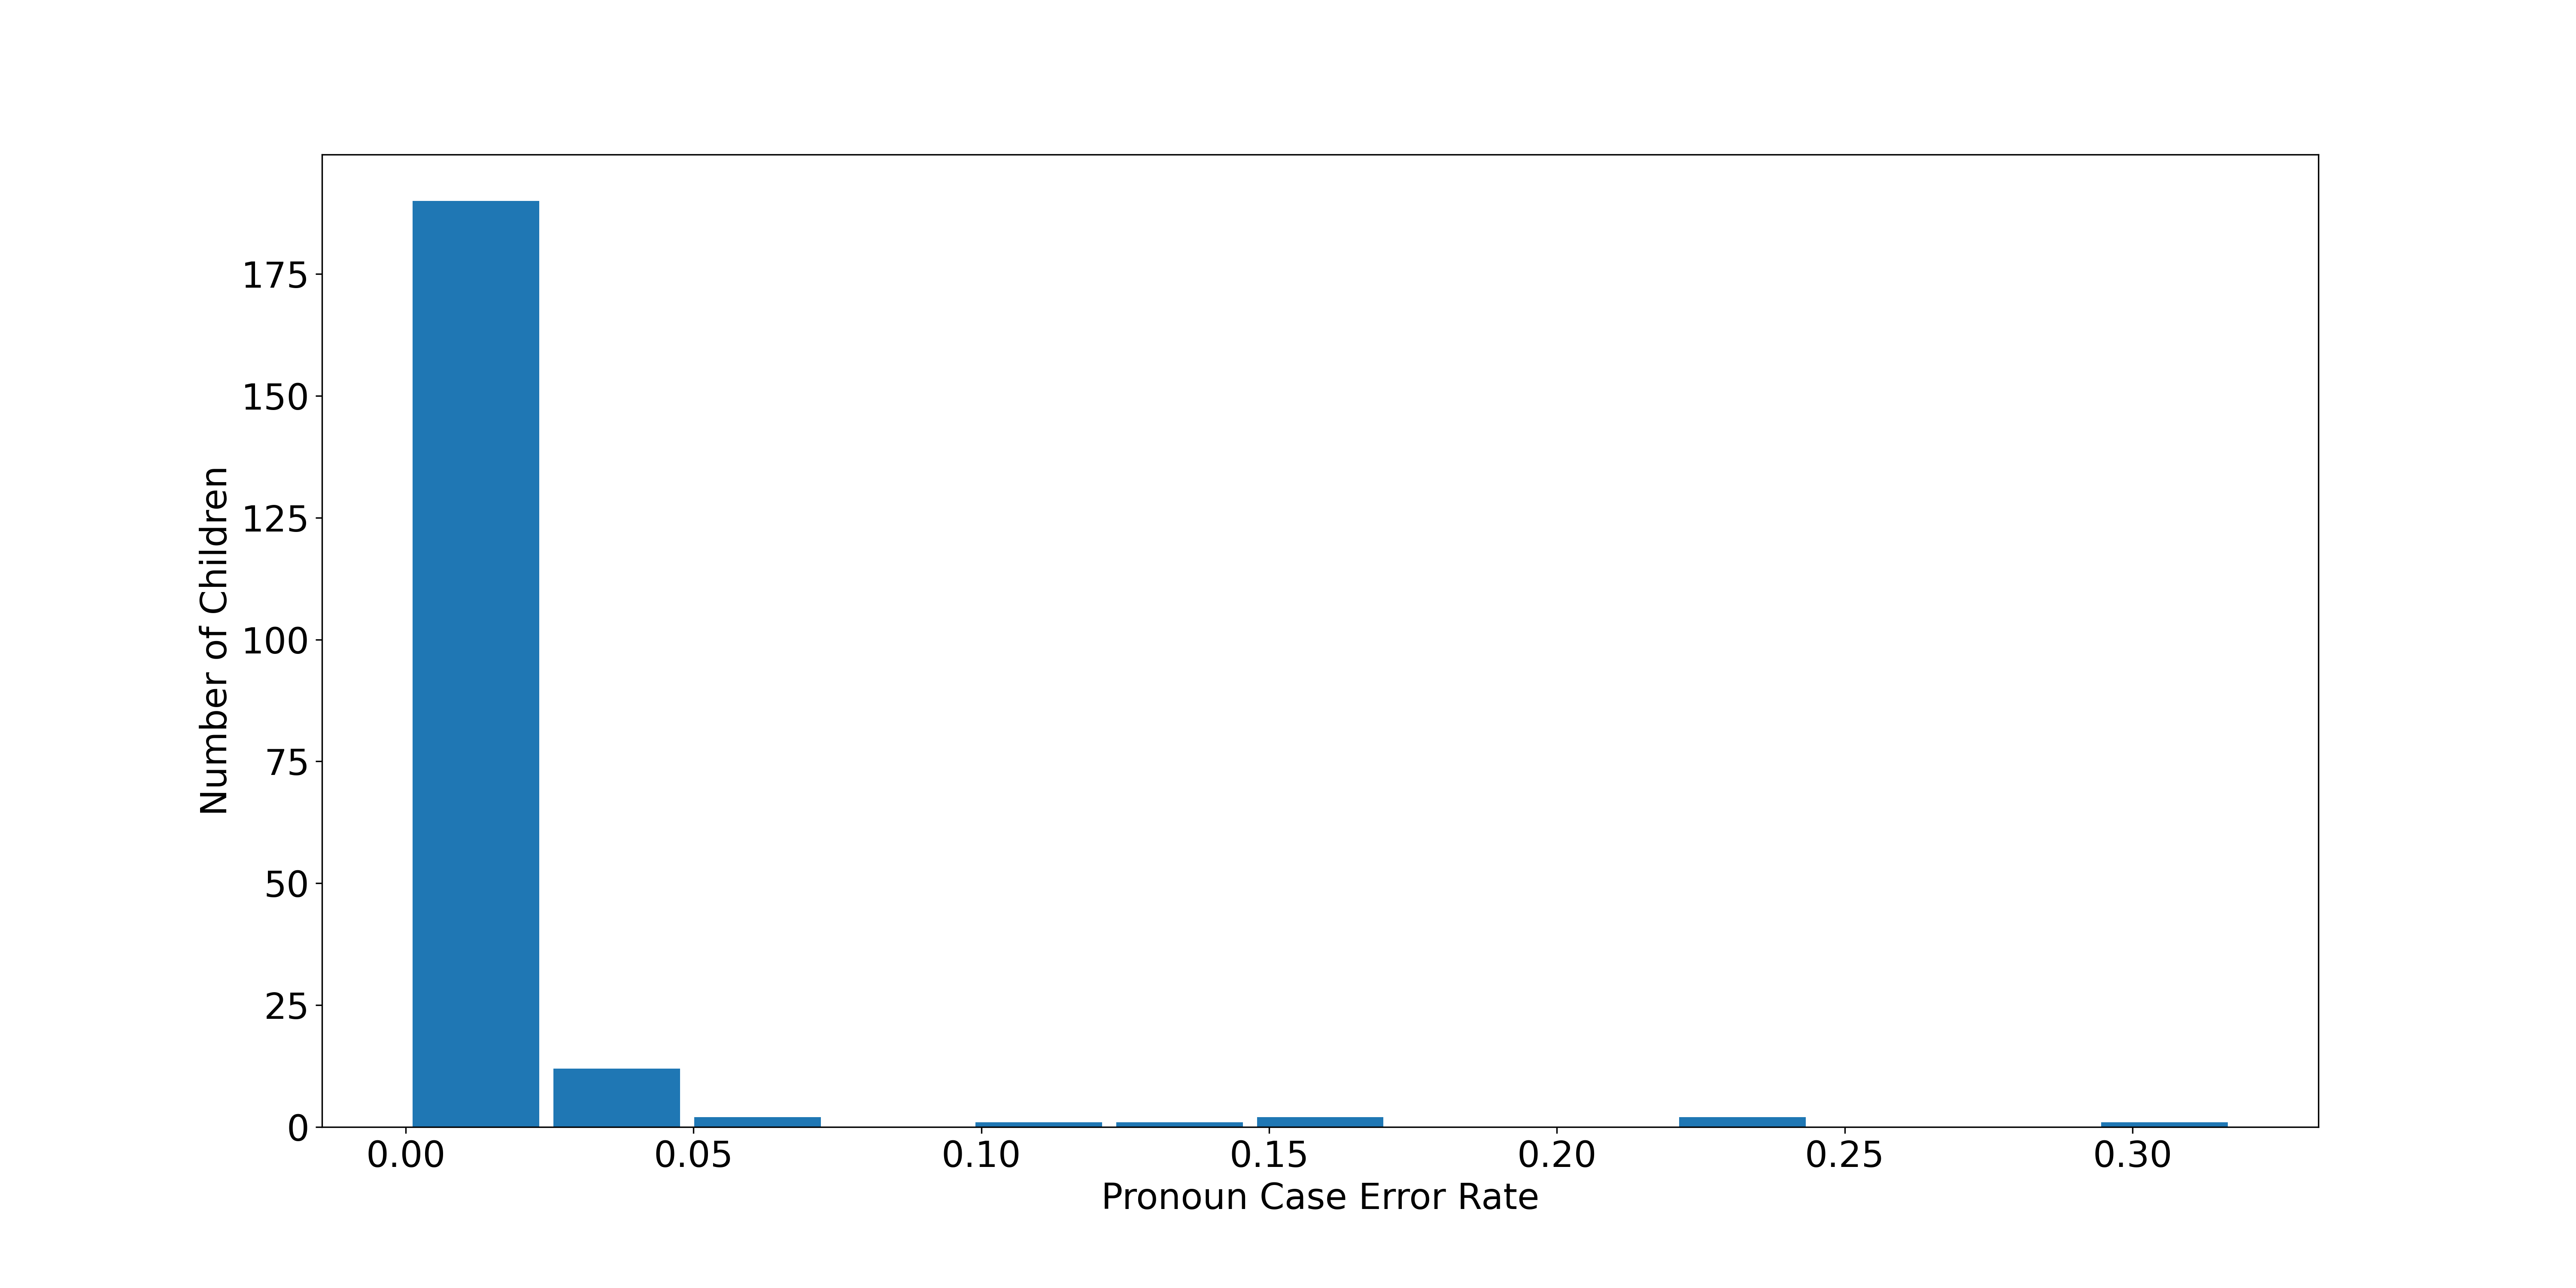
\includegraphics[scale = 0.35]{graph/OverallErrorRate.png}
\vspace{-3em}
\caption{Histogram of pronoun case error rate among 211 children}
\label{fig:212}
\end{figure}
\FloatBarrier
\begin{figure}[h]
\centering
    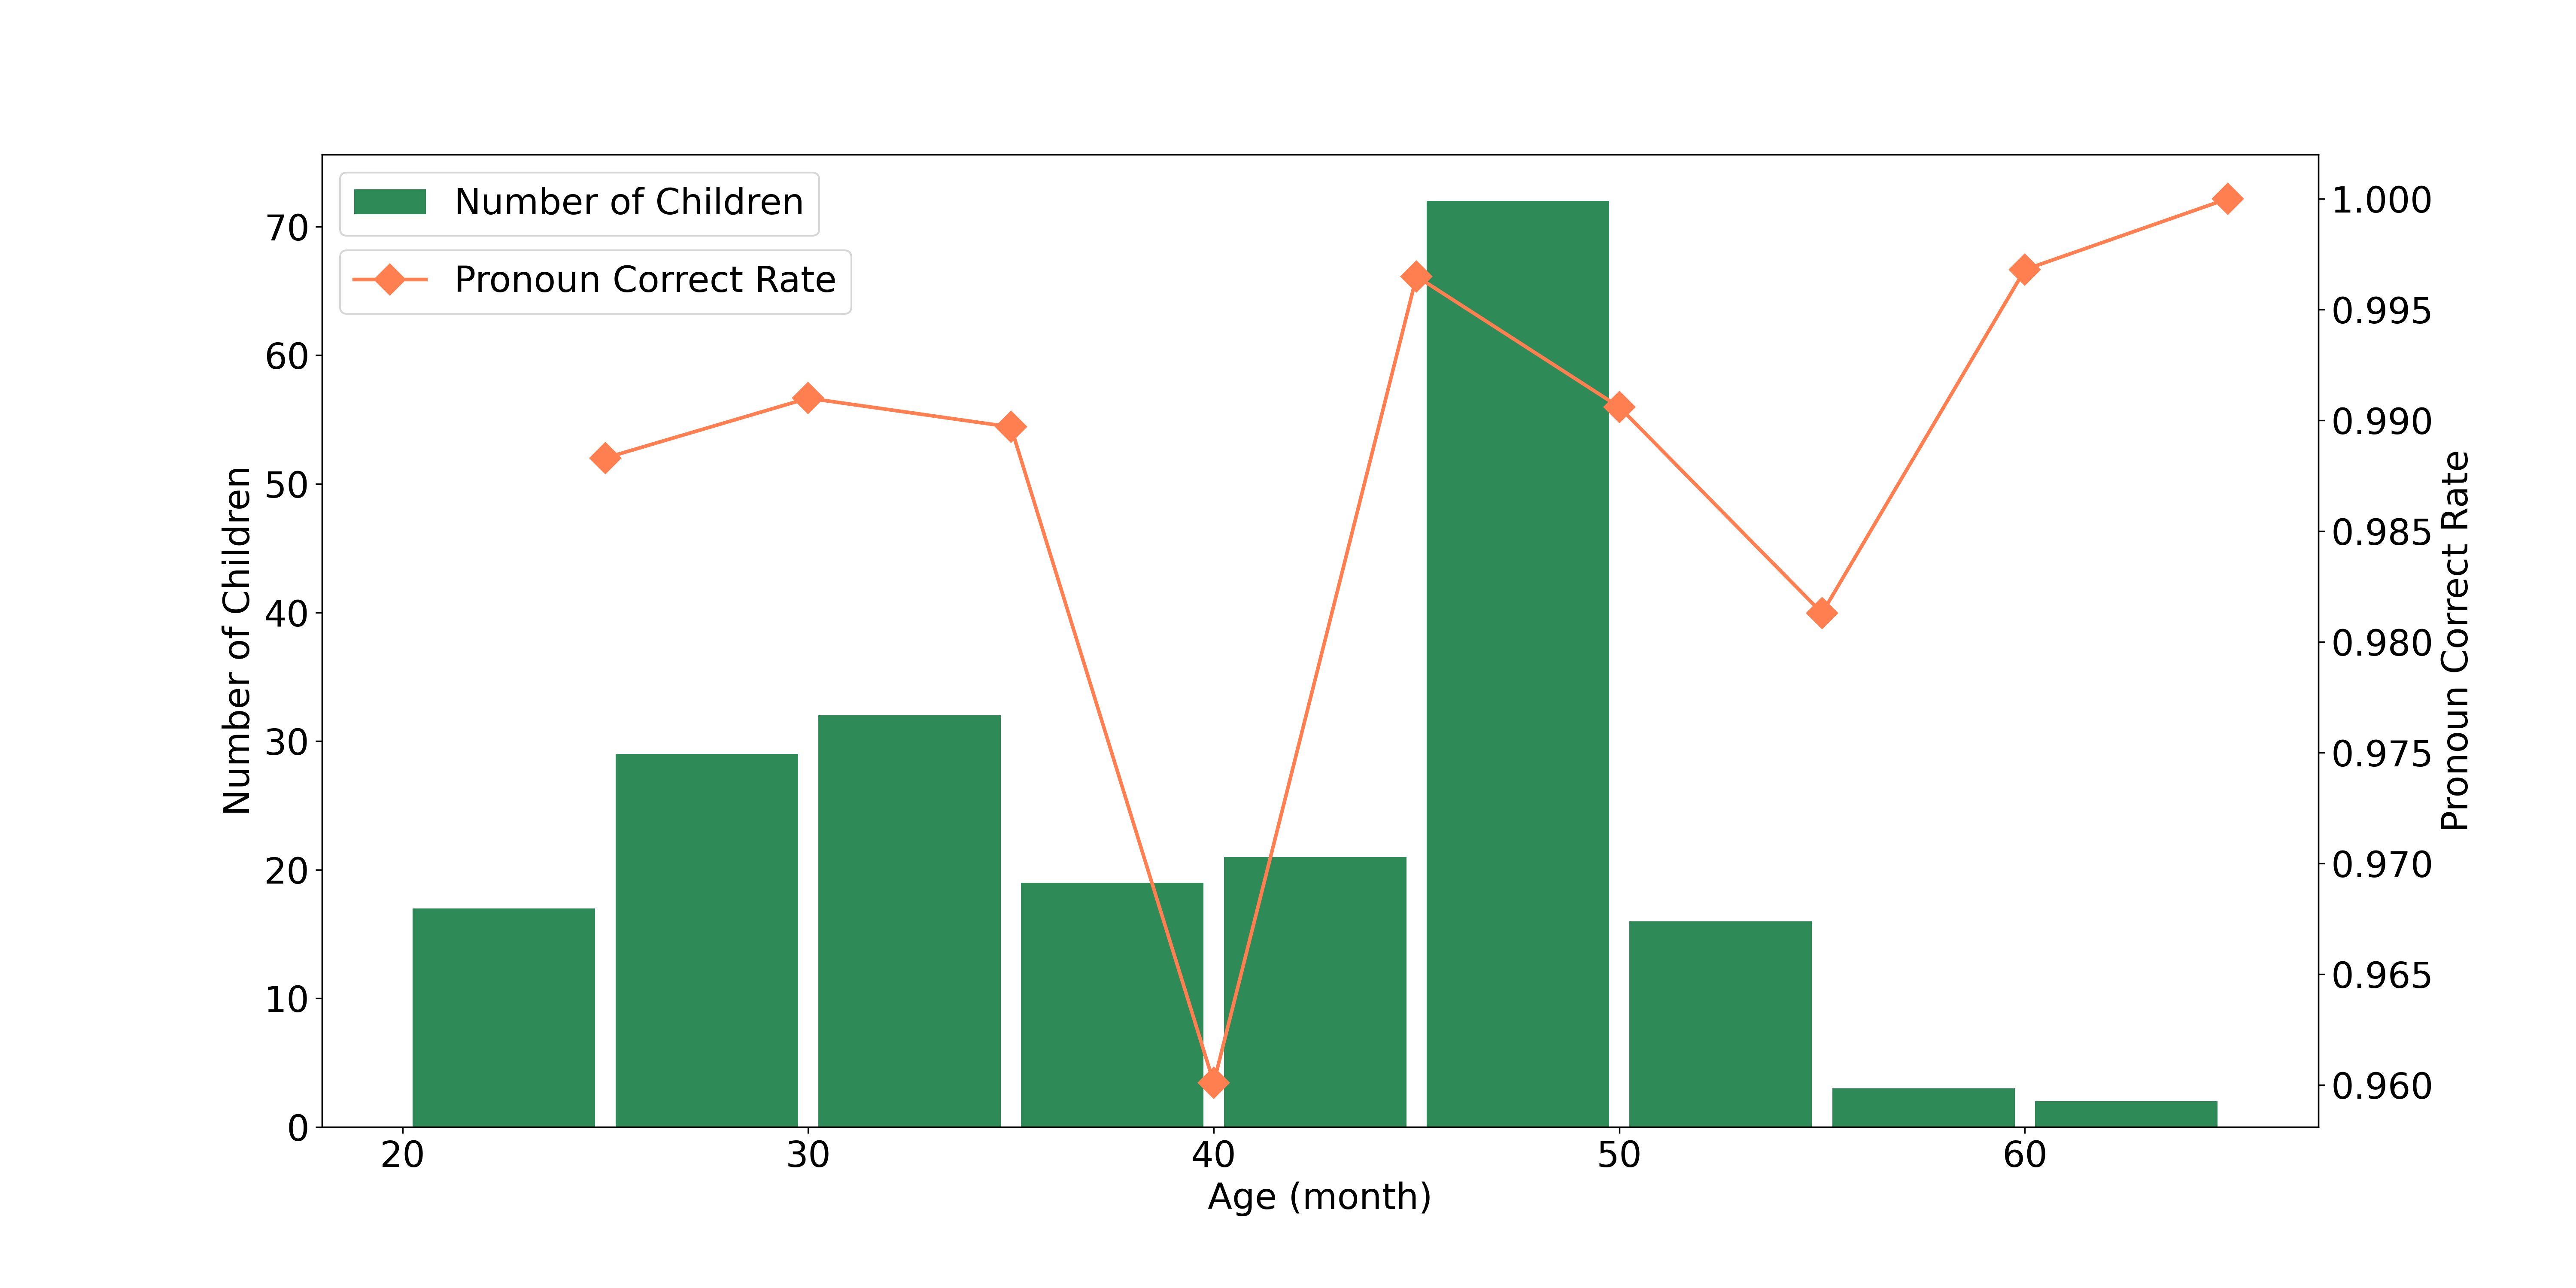
\includegraphics[scale =0.35] {graph/Crosssectional.png}
    \vspace{-3em}
    \caption{Histogram of Age with Pronoun Correct Rate}
    \label{fig:cross}
\end{figure}
\subsubsection{The Rate of Pronoun Case Errors from Longtitudinal Data}
Table \ref{table:2} shows a summary of each longitudinal child's age and MLU range, total number of pronoun and pronoun errors and total number of pronoun produced by their parents. The average pronoun case correct rate is 98.44\% and the median correct rate is 99.40\%, suggesting that most of the children rarely make any pronoun case errors. 

In order to examine if there's a U-shaped pattern for pronoun correct rate, files with the same age month were concatenated as one age point. For example, Eleanor in the dense MPI corpus \citep{rowland2006effect} had 19 files at the age of 2;0. The MLU, children's total pronouns, total input pronouns, total errors and pronoun correct rate are averaged over the 19 files to represent the age point 2;0. First, Spearman's rho test was conducted to calculate the correlation between the pronoun correct rate with age, MLU, children's total pronouns and total input pronouns at each age point. As shown in Table \ref{table:3}, the pronoun correct rate for 46 children has a complicated relationship with age, mlu, children's total words, children's total pronouns and parents' input pronouns. For 27 children, a significant correlation was found between pronoun correct rate VS age, mlu, children's total words, children's total pronouns and input pronouns. 9 children's age and mlu are both positively correlated with pronoun correct rate. 3 children's age and mlu are both negatively correlated with pronoun correct rate. 
3 children's (Fraser, Stuart, She) pronoun correct rate was only positively correlated with age, but not MLU. Nathaniel's pronoun correct rate is only positively correlated with MLU but not age. Conor's MLU is negatively correlated with pronoun correct rate. In addition, the age range doesn't seem to affect the correlation. For example, Aran, Dominic and John from the Manchester corpus \citep{theakston2001} all have the same age range (1;11 - 2;11) and 12 age points; Aran's pronoun correct rate is positively correlated with age and mlu; Dominic's pronoun correct rate is negatively correlated with age and mlu; while there is no significant correlation between John's pronoun correct rate and age or mlu. 

Similarly, both negative and positive correlations were found between pronoun correct rate VS children's total words, children's total pronouns and children's input pronouns; and for more than half of the children, there is no significant correlation between pronoun correct rate VS children's total words, children's total pronouns and children's input pronouns. 

Given that there is no unified monotonic improvement in pronoun correct rate with age and mlu, it is possible that the pronoun correct rate would show a U-shaped pattern on longitudinal data. 9 children with at least 20 age points (Thomas, Laura, Adam, Sarah, Naomi, Ross, Abe, Matt, Roman) were selected for plotting pronoun correct rate and age. The 9 children's age range varies. For example, Ross's age point starts at 1;4 and ends at 7;8, while Abe's age point starts at 2;5 and ends 5;0. To ensure that all 9 children are fairly represented on the graph, the most common age range 2;4 - 5;0 (with 32 age points) was selected. Each child's pronoun correct rate at different age points are plotted in Figure \ref{fig:1}. The detailed data can be found in Table \ref{table:4}. 
\vspace{-1em}
\FloatBarrier
\begin{figure}[!h]
\small
\centering
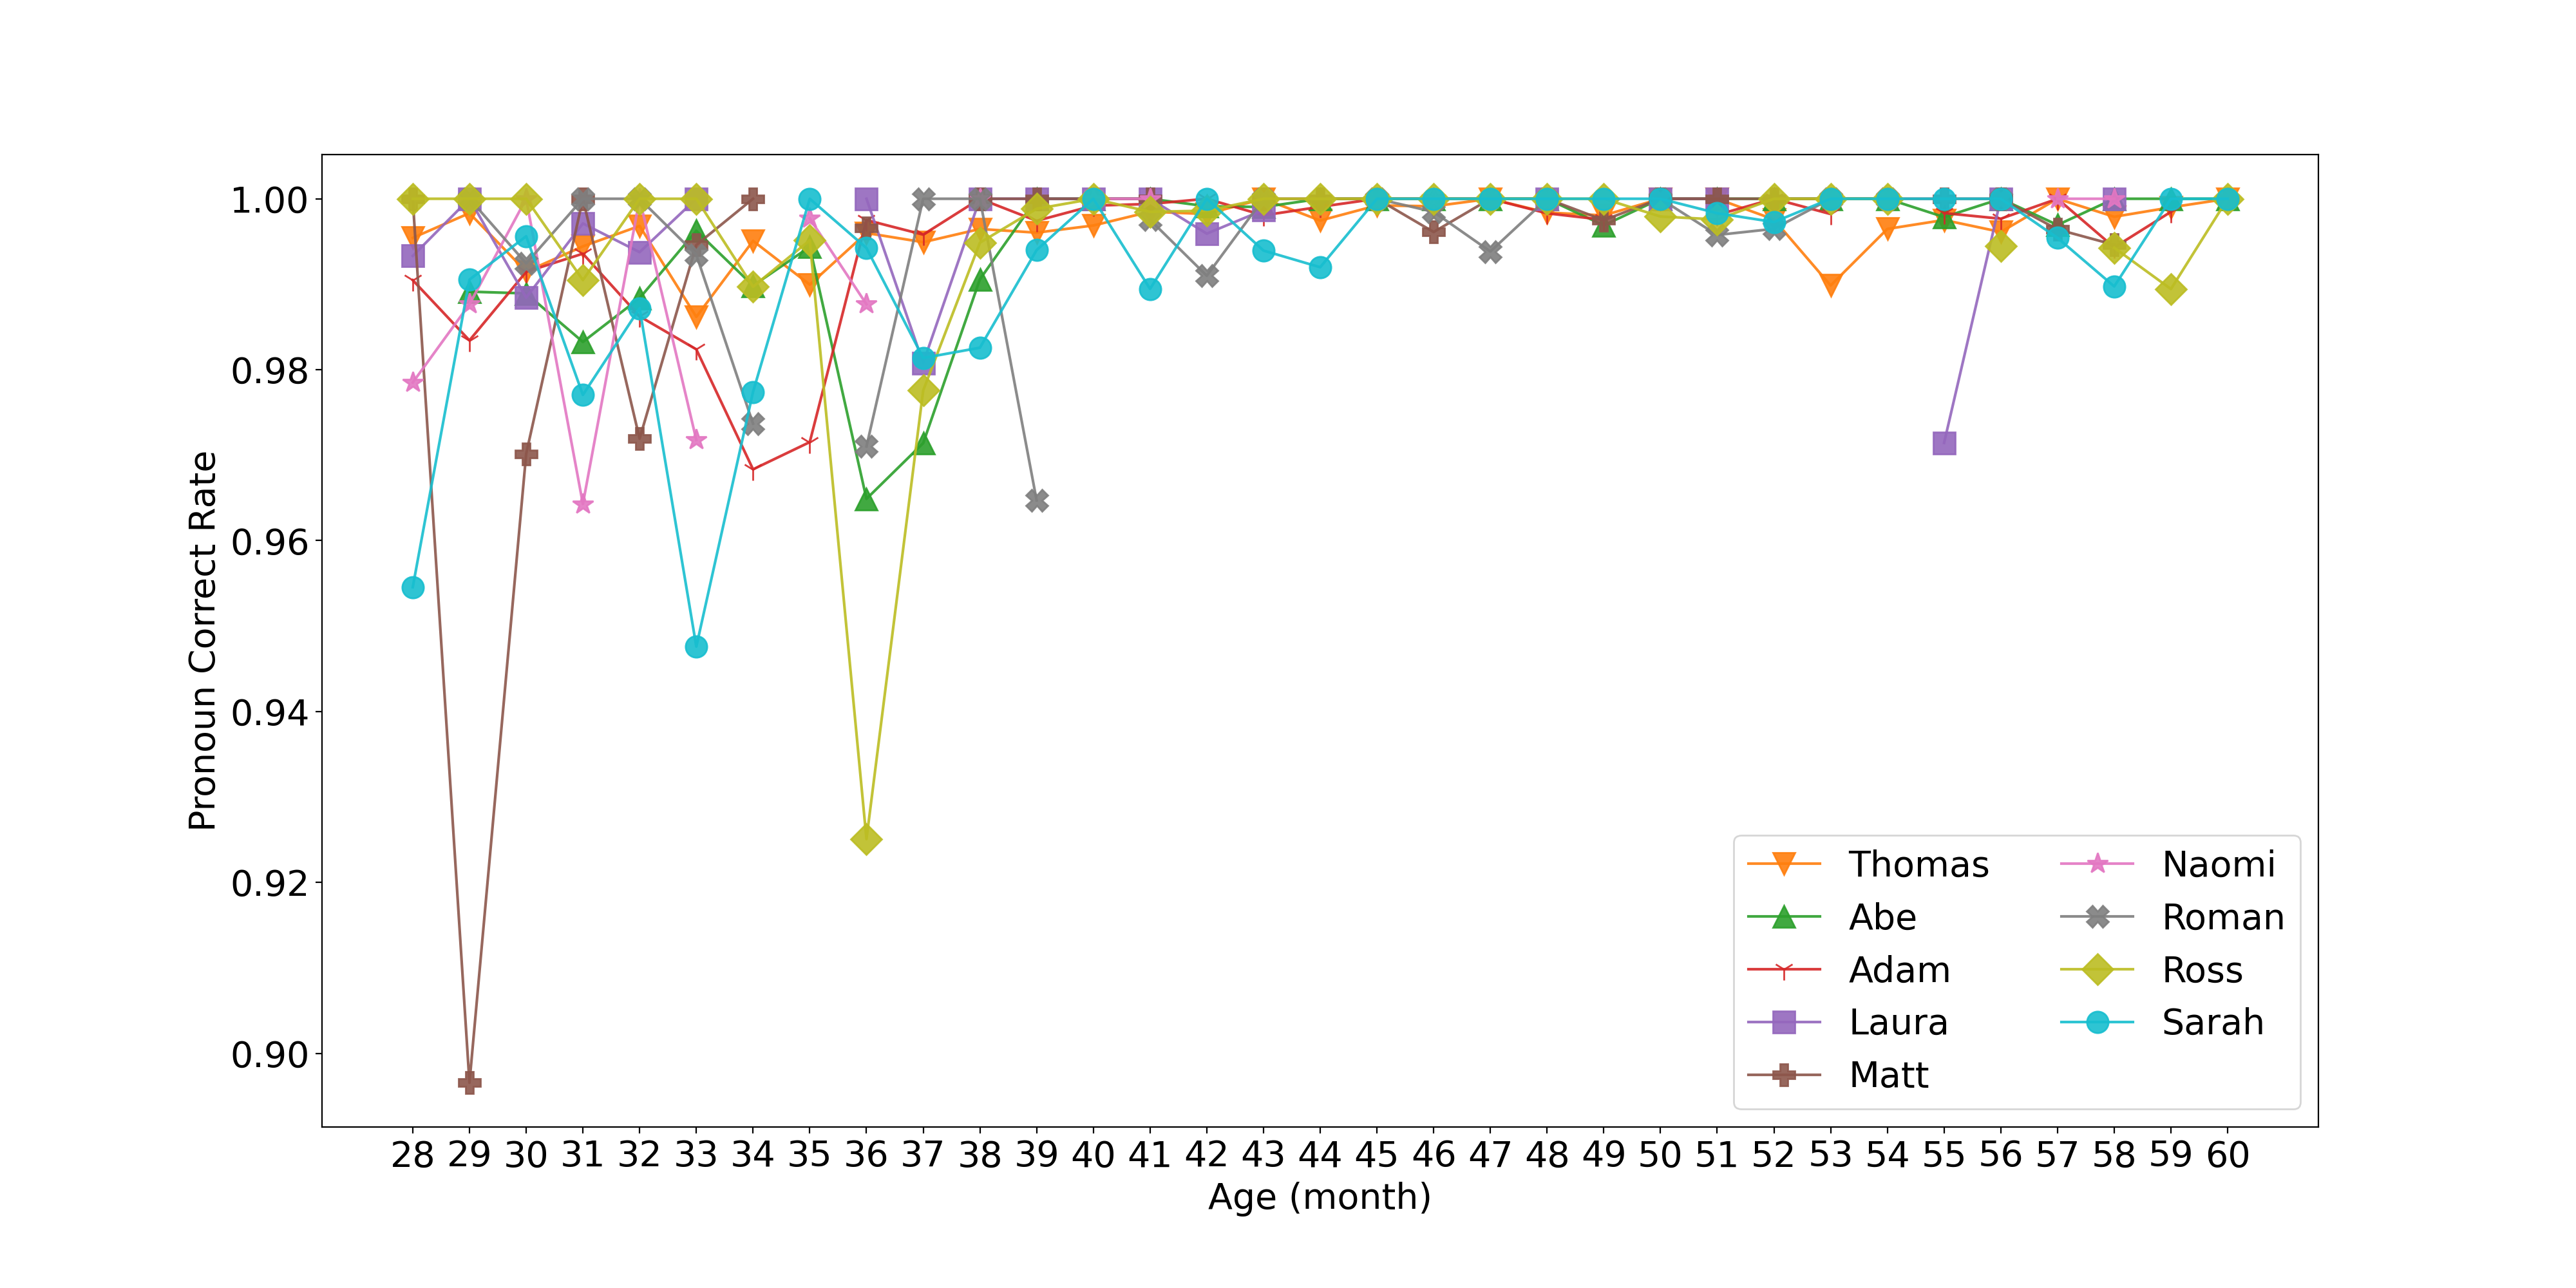
\includegraphics[scale = 0.35, width = \linewidth]{graph/Age1month.png}
\vspace{-2em}
\caption{Age and Pronoun Correct Rate per age point for longitudinal data and cross-sectional data }
\label{fig:1}
\end{figure}
\FloatBarrier

The pronoun correct rate has a very noisy pattern at the early age points and stabilizes roughly after the age point of 3;4 (40 months). To get a clearer visualization for the early age points, the pronoun correct rates were averaged per 5 age points and the new plot is shown in Figure \ref{fig:2}.
\FloatBarrier
\begin{figure}[h]
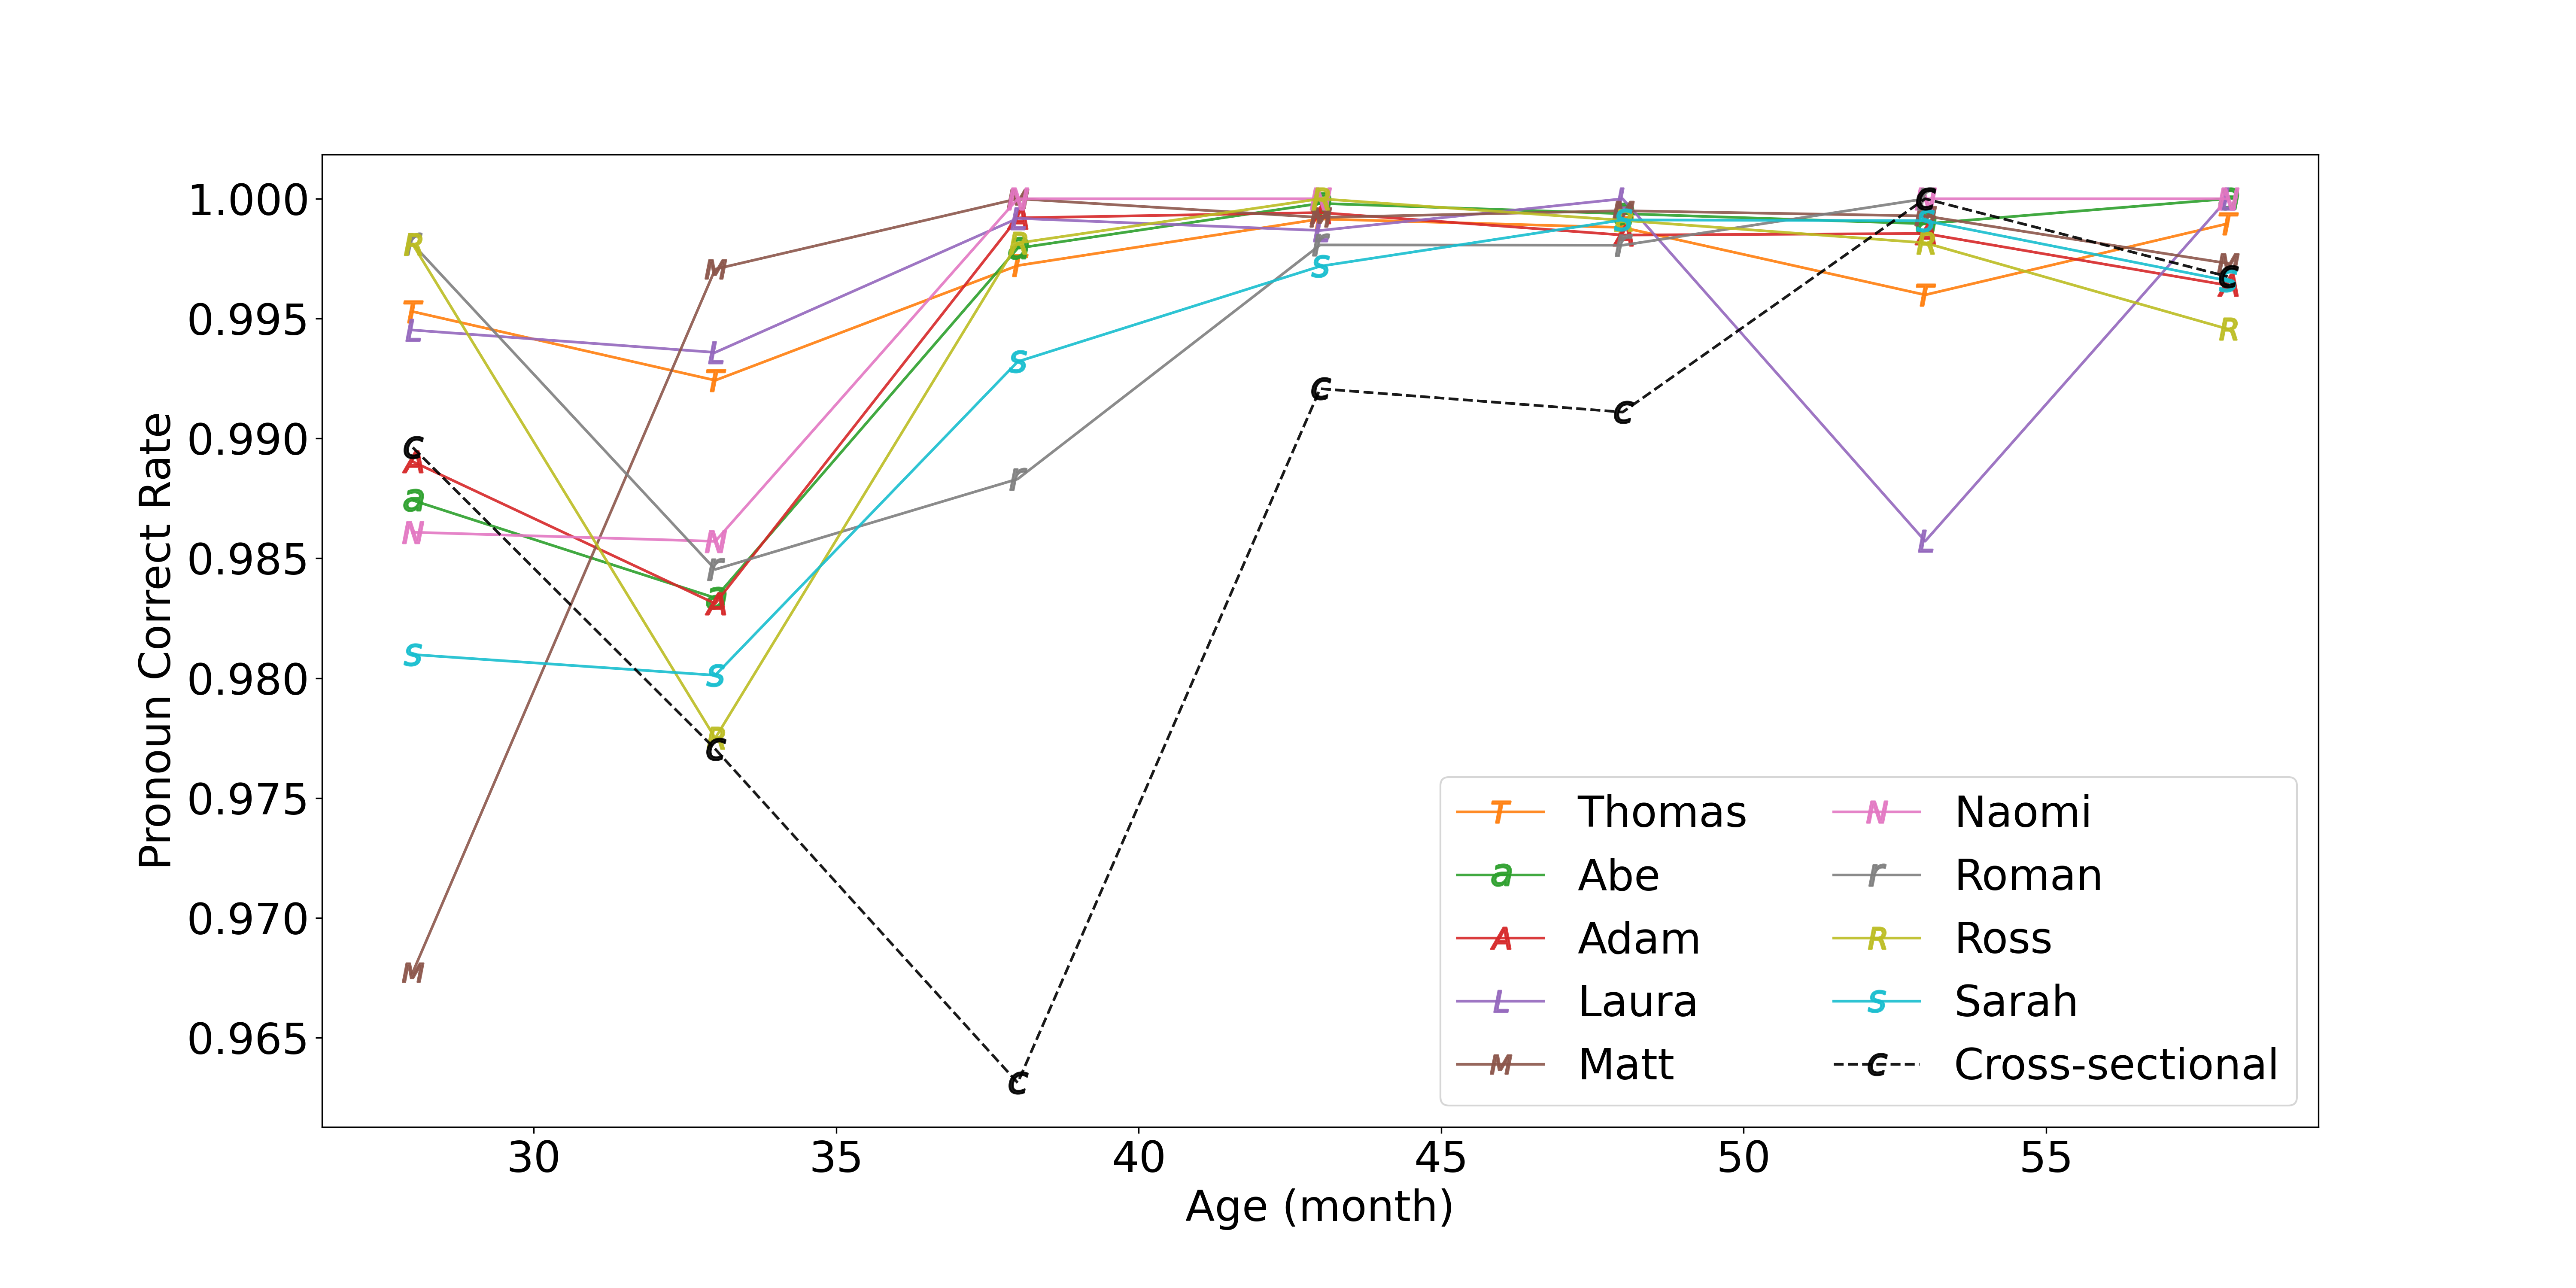
\includegraphics[scale = 0.35, width = \linewidth]{graph/Age5month.png}
\vspace{-2em}
\caption{Age and Pronoun Correct Rate per 5 age points}
\label{fig:2}
\end{figure}
\FloatBarrier
The colored solid lines represent each individual child's pronoun correct rate and the dashed black line represents the cross-sectional data. The longitudinal children's pronoun correct rate seems to resemble a U-shaped pattern, that most children start with a relatively high correct rate and then experience a dip at around age 2;9 (33 months) and return to high correct rate roughly after 3;7 (40 months). However, the position of the dip in longitudinal data is slightly different from the dip in the cross-sectional data: the pronoun correct rate dropped earlier for the children with longitudinal data than the children with cross-sectional data. It is unclear why the pronoun correct rate dropped at different ages for longitudinal children and cross-sectional children. 

\FloatBarrier
\begin{table}[h]
\centering
\small
\caption{Summary of children's age range, mlu range, total pronouns, total input pronouns and total errors}
\label{table:2}
\begin{tabular}{llllllll}
\hline
\textbf{Name} & \textbf{{\begin{tabular}[c]{@{}l@{}}Total\\files \end{tabular}}}\footnote{Diary files were not included in this study. For example, Lara had 225 diary files that were not included in the study.} & \textbf{Age range} & \textbf{MLU range} & \textbf{\begin{tabular}[c]{@{}l@{}}Children's\\ Total\\ Pronoun\end{tabular}} & \textbf{\begin{tabular}[c]{@{}l@{}}Total\\Input\\ pronoun\end{tabular}} & \textbf{{\begin{tabular}[c]{@{}l@{}}Total\\Errors \end{tabular}}} & \textbf{\begin{tabular}[c]{@{}l@{}}Correct \\ Rate\end{tabular}} \\ \hline
Anne & 40 & 1;10 - 2;9 & 1.75 - 4.15 & 4957 & 18707 & 54 & 98.91\% \\
Aran & 53 & 1;11 - 2;11 & 1.46 - 5.02 & 10174 & 43339 & 24 & 99.76\% \\
Barbara & 14 & 2;4 - 4;2 & 3.37 - 6.47 & 1339 & 5052 & 7 & 99.48\% \\
Becky & 35 & 2;0 - 2;11 & 1.53 - 3.97 & 6893 & 14524 & 41 & 99.41\% \\
Carl & 33 & 1;9 - 2;8 & 2.22 - 4.36 & 5446 & 10398 & 32 & 99.41\% \\
Conor & 14 & 3;8 - 4;6 & 1.87 - 5.71 & 1993 & 8051 & 14 & 99.30\% \\
Courtney & 7 & 3;4 - 4;0 & 5.13 - 6.68 & 1398 & 1727 & 6 & 99.57\% \\
David & 14 & 2;0 - 4;2 & 2.32 - 6.41 & 1013 & 3219 & 3 & 99.70\% \\
Dominic & 36 & 1;11 - 2;11 & 1.34 - 4.08 & 4787 & 18519 & 47 & 99.02\% \\
Eleanor & 181 & 2;0 - 3;1 & 2.12 - 4.25 & 28834 & 59462 & 80 & 99.72\% \\
Fraser & 217 & 2;0 - 3;1 & 1.70 - 5.7 & 37480 & 92975 & 67 & 99.82\% \\
Gail & 35 & 2;0 - 2;11 & 1.87 - 4.33 & 4690 & 16029 & 63 & 98.66\% \\
Joel & 35 & 1;11 - 2;10 & 1.41 - 3.92 & 4936 & 15207 & 24 & 99.51\% \\
John & 32 & 1;11 - 2;11 & 1.92 - 3.78 & 2168 & 10276 & 8 & 99.63\% \\
Johnny & 7 & 3;6 - 4;4 & 3.93 - 4.52 & 861 & 507 & 4 & 99.54\% \\
Lara & 125 & 1;9 - 3;4 & 1.85 - 5.35 & 153054 & 40920 & 63 & 99.75\% \\
Liz & 34 & 1;11 - 2;11 & 1.52 - 4.79 & 5048 & 10708 & 31 & 99.39\% \\
Michelle & 14 & 2;5 - 4;5 & 3.0 - 6.87 & 2386 & 3979 & 31 & 98.70\% \\
Nicole & 34 & 2;1 - 3;0 & 1.26 - 3.61 & 2286 & 17860 & 51 & 97.77\% \\
Rachel & 9 & 2;6 - 3;2 & 2.8 - 6.33 & 663 & 2756 & 42 & 93.67\% \\
Ruth & 33 & 1;11 - 3;0 & 1.63 - 4.34 & 4077 & 19657 & 971 & 76.18\% \\
Stuart & 11 & 3;5 - 4;5 & 4.51 - 6.34 & 2352 & 2720 & 22 & 99.06\% \\
Thomas & 379 & 2;0 - 5;0 & 1.55 - 6.92 & 48115 & 226908 & 197 & 99.59\% \\
Warren & 36 & 1;10 - 2;10 & 2.02 - 4.71 & 4008 & 14818 & 96 & 97.60\% \\
Peter & 20 & 1;9 - 3;2 & 1.47 - 6.66 & 7637 & 2527 & 89 & 98.83\% \\
Laura & 200 & 1;5 - 7;0 & 1.0 - 6.69 & 9895 & 14280 & 82 & 99.17\% \\
Adam & 55 & 2;3 - 5;2 & 2.41 - 6.48 & 23726 & 13172 & 90 & 99.62\% \\
Eve & 20 & 1;6 - 2;3 & 2.1 - 4.99 & 4217 & 6458 & 39 & 99.08\% \\
Sarah & 139 & 2;3 - 5;1 & 1.59 - 7.77 & 15344 & 18512 & 110 & 99.28\% \\
Jimmy & 26 & 2;2 - 2;10 & 3.51 - 5.8 & 2702 & 3736 & 31 & 98.85\% \\
Shem & 47 & 2;3 - 3;2 & 4.32 - 12.03 & 9176 & 2207 & 19 & 99.79\% \\
Naomi & 93 & 1;3 - 4;9 & 1.3 - 7.79 & 5200 & 6466 & 60 & 98.85\% \\
Ross & 409 & 1;4 - 7;8 & 1.7 - 21.25 & 24560 & 41774 & 99 & 99.60\% \\
She & 10 & 1;8 - 2;5 & 2.23 - 3.54 & 706 & 2355 & 21 & 97.03\% \\
Tow & 10 & 1;7 - 2;5 & 1.86 - 5.08 & 946 & 3790 & 34 & 96.41\% \\
Nina & 52 & 2;0 - 3;4 & 2.26 - 6.17 & 11740 & 25694 & 501 & 95.73\% \\
Abe & 210 & 2;5 - 5;0 & 3.69 - 10.58 & 24547 & 18526 & 130 & 99.47\% \\
Trevor & 26 & 2;1 - 4;0 & 4.28 - 8.12 & 2819 & 5222 & 17 & 99.40\% \\
Ben & 11 & 2;4 - 3;4 & 4.97 - 6.88 & 1634 & 1177 & 50 & 96.94\% \\
Emily & 23 & 2;6 - 4;6 & 4.66 - 9.54 & 5067 & 144 & 15 & 99.70\% \\
Emma & 27 & 2;8 - 4;8 & 3.71 - 6.4 & 3458 & 2648 & 5 & 99.86\% \\
Jillian & 22 & 2;1 - 2;10 & 2.76 - 7.16 & 2669 & 2795 & 5 & 99.81\% \\
Matt & 57 & 2;3 - 5;0 & 2.89 - 11.29 & 6586 & 19759 & 34 & 99.48\% \\
Roman & 42 & 2;3 - 4;8 & 2.98 - 12.11 & 6047 & 4745 & 33 & 99.45\% \\
Nathaniel & 47 & 2;6 - 3;9 & 1.82 - 6.45 & 2193 & 10329 & 14 & 99.36\% \\
Geraldine & 10 & 1;6 - 2;5 & 1.35 - 5.43 & 598 & 1945 & 3 & 99.50\% \\ \hline
\end{tabular}
\end{table}
\FloatBarrier

\FloatBarrier
\begin{table}[]
\small
\centering
\caption{Spearman's Correlation between Pronoun Correct Rate and Age, MLU, Children's total word production, Children's pronoun production, Total Input Pronouns}
\label{table:3}
\begin{tabular}{ll|lllll}
\toprule
 & &\multicolumn{5}{c}{\textbf{Correlation (r) with Pronoun Correct Rate}} \\
\hline
\textbf{Child} & \textbf{{\begin{tabular}[c]{@{}l@{}}N (age points)\\(age range)\end{tabular}}}& \textbf{Age} & \textbf{MLU} & \textbf{\begin{tabular}[c]{@{}l@{}}Children's\\ Total Words\end{tabular}} & \textbf{\begin{tabular}[c]{@{}l@{}}Children's\\ Total Pronouns\end{tabular}} & \textbf{\begin{tabular}[c]{@{}l@{}}Total Input\\ Pronouns\end{tabular}}\\
\hline
Anne&11 (1;10 - 2;9)&-0.16&-0.04&-0.38&-0.33&-0.29\\
Aran&12 (1;11 - 2;11)&\textbf{0.77**}&\textbf{0.68*}&\textbf{0.79**}&\textbf{0.78**}&-0.05\\
Barbara&10 (2;4 - 4;2)&-0.14&0.3&-0.12&-0.08&-0.08\\
Becky&12 (2;0 - 2;11)&-0.36&-0.57&-0.31&-0.34&0.49\\
Carl&12 (1;9 - 2;8)&-0.07&0.22&0.19&-0.02&0.42\\
Conor&9 (3;8 - 4;6)&-0.34&\textbf{-0.94***}&-0.38&-0.42&-0.43\\
Courtney&5 (3;4 - 4;0)&0&0&-0.35&-0.35&0\\
David&12 (2;0 - 4;2)&-0.16&-0.23&-0.44&-0.38&0.19\\
Dominic&12 (1;11 - 2;11)&\textbf{-0.77**}&\textbf{-0.77**}&\textbf{-0.62*}&\textbf{-0.81**}&-0.46\\
Eleanor&14 (2;0 - 3;1)&0.45&0.42&0.5&0.52&\textbf{0.83***}\\
Fraser&14 (2;0 - 3;1)&\textbf{0.60*}&0.5&0.42&\textbf{0.57*}&\textbf{0.57*}\\
Gail&11 (2;0 - 2;11)&0.35&0.25&\textbf{-0.43*}&-0.11&\textbf{0.51*}\\
Joel&11 (1;11 - 2;10)&0.12&0.09&0.31&0.11&\textbf{0.75**}\\
John&12 (1;11 - 2;11)&0&-0.02&-0.35&-0.11&0.08\\
Johnny&5 (3;6 - 4;4)&-0.15&-0.67&-0.36&-0.67&-0.67\\
Lara&19 (1;9 - 3;4)&\textbf{0.61**}&\textbf{0.60**}&0.3&\textbf{0.55*}&0.33\\
Liz&12 (1;11 - 2;11)&0.46&0.39&-0.12&0.15&-0.35\\
Michelle&9 (2;5 - 4;5)&-0.39&-0.14&-0.31&-0.31&0.29\\
Nicole&11 (2;1 - 3;0)&\textbf{-0.85***}&\textbf{-0.85***}&\textbf{-0.76***}&\textbf{-0.82***}&-0.11\\
Rachel&5 (2;6 - 3;2)&0.72&0.87&-0.87&-0.36&0.1\\
Ruth&13 (1;11 - 3;0)&0.4&0.45&0.36&0.33&0.51\\
Stuart&7 (3;5 - 4;5)&\textbf{0.83*}&0.09&-0.25&-0.11&-0.04\\
Thomas&36 (2;0 - 5;0)&\textbf{0.51**}&\textbf{0.58**}&\textbf{0.39*}&\textbf{0.39*}&0.1\\
Warren&12 (1;10 - 2;10)&0.05&-0.03&0.09&0.24&0.29\\
Peter&14 (1;9 - 3;2)&0.11&0.15&0.07&0.09&-0.37\\
Laura&34 (1;5 - 7;0)&\textbf{0.60***}&\textbf{0.48**}&\textbf{0.57***}&\textbf{0.50**}&\textbf{0.40*}\\
Adam&31 (2;3 - 5;2)&\textbf{0.61***}&\textbf{0.62***}&\textbf{0.50**}&\textbf{0.45*}&0.11\\
Eve&10 (1;6 - 2;3)&\textbf{-0.74*}&\textbf{-0.69*}&\textbf{-0.66*}&\textbf{-0.67*}&-0.02\\
Sarah&35 (2;3 - 5;1)&\textbf{0.63***}&\textbf{0.60***}&\textbf{0.46**}&0.28&0.04\\
Jimmy&6 (2;2 - 2;10)&-0.6&-0.6&0.31&-0.09&0.31\\
Shem&12 (2;3 - 3;2)&0.04&-0.03&0.04&0.25&0.39\\
Naomi&23 (1;3 - 4;9)&\textbf{0.42*}&\textbf{0.43*}&0.25&0.33&0.18\\
Ross&62 (1;4 - 7;8)&0.14&-0.07&-0.17&-0.19&0.09\\
She&9 (1;8 - 2;5)&\textbf{0.78*}&0.57&0.45&\textbf{0.72*}&0.52\\
Tow&9 (1;7 - 2;5)&0.31&0.29&0&0&-0.15\\
Nina&15 (2;0 - 3;4)&\textbf{0.83***}&\textbf{0.86***}&\textbf{0.62*}&\textbf{0.68**}&0.26\\
Abe&32 (2;5 - 5;0)&\textbf{0.69***}&\textbf{0.38*}&-0.26&-0.24&\textbf{-0.46**}\\
Trevor&10 (2;1 - 4;0)&0.01&-0.49&-0.07&-0.05&0.25\\
Ben&8 (2;4 - 3;4)&0.36&0.4&-0.19&0.5&\textbf{0.71*}\\
Emily&13 (2;6 - 4;6)&0.07&-0.18&-0.4&-0.37&-0.25\\
Emma&16 (2;8 - 4;8)&0.47&0.41&0.44&0.43&-0.21\\
Jillian&7 (2;1 - 2;10)&-0.08&-0.16&-0.45&-0.35&0.37\\
Matt&29 (2;3 - 5;0)&0.27&0.28&0.29&0.11&0.09\\
Roman&24 (2;3 - 4;8)&0.15&-0.06&-0.19&-0.07&0.17\\
Nathaniel&10 (2;6 - 3;9)&0.35&\textbf{0.63*}&0.12&0.52&0.22\\
Geraldine&7 (1;6 - 2;5)&0.4&0.4&-0.04&0.09&0.04\\
\bottomrule
\end{tabular}
\end{table}
\FloatBarrier


\FloatBarrier
\begin{table}[h]
\small
\centering
\caption{Pronoun Correct Rate at each age points for 9 children}
\label{table:4}
\begin{tabular}{c|lllllllll}
\hline
\textbf{{\begin{tabular}[c]{@{}c@{}}Age\\(month)\end{tabular}}} & \textbf{Thomas} & \textbf{Abe} & \textbf{Adam} & \textbf{Laura} & \textbf{Matt} & \textbf{Naomi} & \textbf{Roman} & \textbf{Ross} & \textbf{Sarah} \\ 
\toprule
28 & 0.9954 & N/A & 0.9905 & 0.9933 & 1 & 0.9785 & N/A & 1 & 0.9545 \\
29 & 0.9983 & 0.9891 & 0.9834 & 1 & 0.8966 & 0.9877 & 1 & 1 & 0.9905 \\
30 & 0.9915 & 0.9889 & 0.9915 & 0.9884 & 0.9701 & 1 & 0.9924 & 1 & 0.9956 \\
31 & 0.9944 & 0.9832 & 0.9936 & 0.9971 & 1 & 0.9643 & 1 & 0.9905 & 0.9770 \\
32 & 0.9968 & 0.9884 & 0.9862 & 0.9938 & 0.9719 & 1 & 1 & 1 & 0.9872 \\
33 & 0.9862 & 0.9962 & 0.9824 & 1 & 0.9946 & 0.9718 & 0.9934 & 1 & 0.9476 \\
34 & 0.9951 & 0.9898 & 0.9683 & N/A & 1 & N/A & 0.9737 & 0.9897 & 0.9774 \\
35 & 0.9900 & 0.9944 & 0.9715 & N/A & N/A & 0.9977 & N/A & 0.9951 & 1 \\
36 & 0.9960 & 0.9649 & 0.9975 & 1 & 0.9966 & 0.9877 & 0.9710 & 0.9251 & 0.9942 \\
37 & 0.9949 & 0.9714 & 0.9958 & 0.9808 & N/A & N/A & 1 & 0.9776 & 0.9814 \\
38 & 0.9965 & 0.9906 & 1 & 1 & 1 & 1 & 1 & 0.9949 & 0.9826 \\
39 & 0.9960 & 1 & 0.9974 & 1 & 1 & N/A & 0.9647 & 0.9988 & 0.9940 \\
40 & 0.9969 & 1 & 0.9992 & 1 & 1 & 1 & N/A & 1 & 1 \\
41 & 0.9985 & 1 & 0.9994 & 1 & 1 & 1 & 0.9975 & 0.9985 & 0.9895 \\
42 & 0.9982 & 0.9991 & 1 & 0.9959 & N/A & N/A & 0.9910 & 0.9986 & 1 \\
43 & 1 & 0.9990 & 0.9981 & 0.9987 & 1 & N/A & 1 & 1 & 0.9939 \\
44 & 0.9974 & 1 & 0.9991 & N/A & 1 & N/A & N/A & 1 & 0.9920 \\
45 & 0.9992 & 1 & 1 & N/A & 1 & N/A & 1 & 1 & 1 \\
46 & 0.9991 & 1 & 1 & N/A & 0.9961 & 1 & 0.9985 & 1 & 1 \\
47 & 1 & 1 & 1 & N/A & 1 & N/A & 0.9938 & 1 & 1 \\
48 & 0.9984 & 1 & 0.9983 & 1 & 1 & N/A & 1 & 1 & 1 \\
49 & 0.9981 & 0.9969 & 0.9975 & N/A & 0.9975 & N/A & N/A & 1 & 1 \\
50 & 1 & 1 & N/A & 1 & 1 & N/A & 1 & 0.9979 & 1 \\
51 & 1 & 1 & 0.9981 & 1 & 1 & N/A & 0.9958 & 0.9976 & 0.9983 \\
52 & 0.9976 & 1 & 1 & N/A & 1 & N/A & 0.9965 & 1 & 0.9973 \\
53 & 0.9899 & 1 & 0.9982 & N/A & 1 & N/A & 1 & 1 & 1 \\
54 & 0.9965 & 1 & N/A & N/A & 1 & N/A & 1 & 1 & 1 \\
55 & 0.9975 & 0.9979 & 0.9983 & 0.9714 & 1 & N/A & N/A & N/A & 1 \\
56 & 0.9961 & 1 & 0.9977 & 1 & 1 & N/A & 1 & 0.9945 & 1 \\
57 & 1 & 0.9969 & 1 & N/A & 0.9964 & 1 & N/A & N/A & 0.9954 \\
58 & 0.9979 & 1 & 0.9943 & 1 & 0.9946 & 1 & N/A & 0.9943 & 0.9897 \\
59 & 0.9990 & 1 & 0.9985 & N/A & N/A & N/A & N/A & 0.9894 & 1 \\
60 & 1 & 1 & N/A & N/A & 1 & N/A & N/A & 1 & 1 \\ 
\bottomrule
\end{tabular}
\end{table}
\FloatBarrier

\subsubsection{Do Pronoun Case Errors Display a U-shaped Pattern?}
The U-shaped developmental trajectory has been observed in a wide variety of learning contexts \citep[for a review, see][]{siegler2004u}. It is especially interesting in language development since it contradicts the idea that language acquisition is monotonic. If the pronoun case errors display a U-shaped pattern, explanations for such errors should account for the non-monotonic developmental pattern too, which provides an important criterion to evaluate the effectiveness of different explanations. 

It's difficult to judge whether the pronoun case errors follow a U-shaped pattern. One challenge is that there is no accurate definition of the U-shaped developmental curve. It has been loosely described as a three-step process: good performance followed by bad performance followed by good performance again. However, it's difficult to decide what is good performance and what is bad performance in the pronoun case error context where most of the children have an extremely low error rate. In Figure \ref{fig:2}, the plot does display the shape of `U', but the difference between the nadir (96.5\%) and the zenith (100\%) is so small that it is unclear whether there is meaningful improvement.

Most studies reporting a U-shaped developmental pattern did not plot the detailed correct rate with age to demonstrate that there is a U-shaped pattern. Instead, they showed that the performance at a later age is significantly worse than an earlier age, but eventually gets better. For example, \cite{namy2004changing} reported that both an 18-month group and a 4-year-old group had better performance on mapping arbitrary gestures than a 26-month-old group. In order to test if the pronoun correct rate at a certain age is  worse the other ages, all the months in cross-sectional data were divided into 7 groups with 5 months apart to ensure that each group have enough samples. Table \ref{table:KW} shows the mean and median pronoun correct rate for 7 different age groups. Since the error rates are not normally distributed and the sample size N for each group is different, a Kruskal-Wallis test (or one-way ANOVA on ranks) was used to compare the correct rate in different groups. The test result shows that there is no significant difference in pronoun correct rate among age groups, H(6) = 8.57, p = 0.20. This result suggests that even there is a dip of pronoun correct rate at around 2;9 - 3;2, the change is not significant. 
\FloatBarrier
\begin{table}[h]
\centering
\caption{Mean and Median Pronoun Correct Rate for 7 age groups }
\label{table:KW}
\begin{tabular}{llll}
\toprule
\begin{tabular}[c]{@{}c@{}}Age Group \\(month)\end{tabular} & N & Mean & Median \\
\hline
\textless{}26 & 18 & 98.83\% & 100\% \\
26 - 30 & 35 & 99.06\% & 100\%\\
31 - 35 & 29 & 98.97\% & 100\%\\
36 - 40 & 18 & 96.01\% & 100\% \\
41 - 45 & 32 & 99.65\% & 100\% \\
46 - 50 & 65 & 99.06\% & 100\% \\
\textgreater{}50 & 14 & 98.71\% & 100\%\\
\bottomrule
\end{tabular}
\end{table}
\FloatBarrier

In addition, a polynominal function was fitted onto the cross-sectional data. A significant quadratic component can be counted as an evidence for a U-shaped pattern. The fitted plot in Figure \ref{poly1} shows that the quadratic regression doesn't fit the cross-sectional data, $R^2$ = 0.006, F(2,208) = 0.58, p = 0.56.
\vspace{-1em}
\FloatBarrier
\begin{figure}[h]
    \centering
    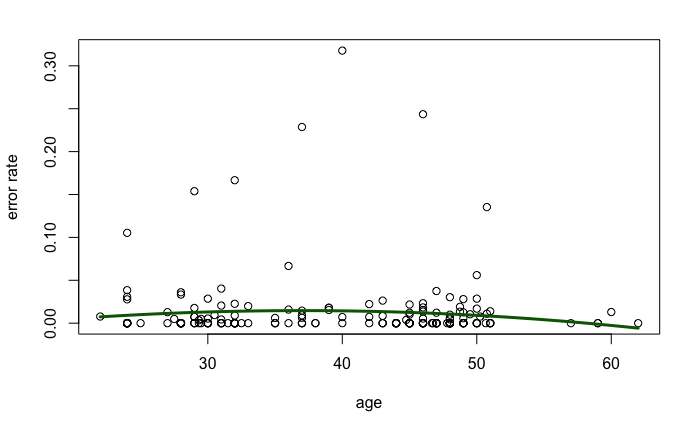
\includegraphics[scale = 0.5]{graph/polynominal1.png}
    \vspace{-1em}
    \caption{Quadratic Function for All Cross-sectional Data Points}
    \label{poly1}
\end{figure}
\FloatBarrier
One reason that the fitting is bad could be that the outliers, data points were the error rate is larger than 0.1, affect the fitting. Therefore, the quadratic function was fitted onto the cross-sectional data without data points with error rates larger than 0.1. The fitted plot is shown in Figure (\ref{poly2}), with $R^2$ = 0.001, F(2,201) = 0.09, p = 0.92. Excluding the outliers didn't improve the model.
\FloatBarrier
\begin{figure}[h]
    \centering
    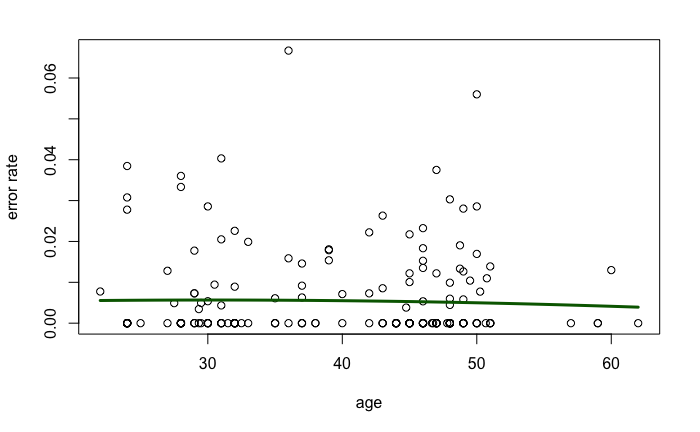
\includegraphics[scale = 0.5]{graph/polynominal2.png}
        \vspace{-1em}
    \caption{Quadratic Function for Cross-sectional Data without Error Rates < 0.1}
    \label{poly2}
\end{figure}
\FloatBarrier
Another reason for the poor fitting of quadratic regression could be that many children have 0 error rate. Therefore, the quadratic function was fitted onto the cross-sectional data without 0 error rate points. The fitted plot in Figure (\ref{poly3}) shows that excluding 0 error rate data points still couldn't make quadratic regression a good fitting model, $R^2$ = 0.01, F(2, 68) = 0.37, p = 0.69.
\FloatBarrier
\begin{figure}[h]
    \centering
    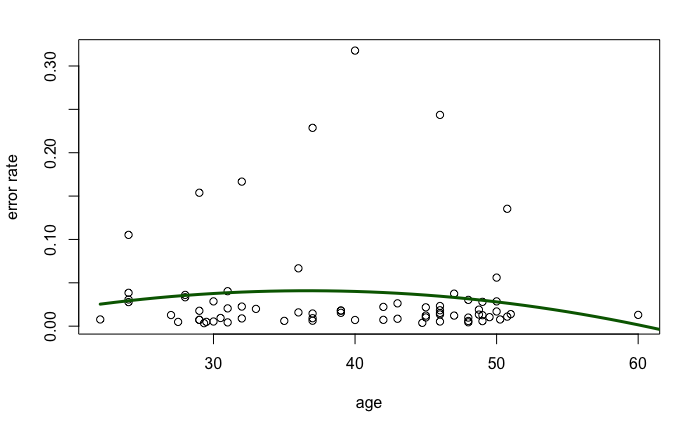
\includegraphics[scale = 0.5]{graph/polynomial3.png}
    \vspace{-1em}
    \caption{Quadratic Function for Cross-sectional Data without 0 Error Rates}
    \label{poly3}
\end{figure}
\FloatBarrier
The results of the Kruskal-Wallis test and the quadratic function fitting suggests that even though there is a dip in the pronoun case correct rate at around 2;9-3;2, the change is not significant. Based on the cross-sectional data, it's difficult to conclude that there is a U-shaped pattern. 


For longitudinal data, since there are not enough samples for different age groups,  Kruskal-Wallis test can not be used to test if the pronoun correct rate is significantly different at different ages. Instead, the longitudinal change in the pronoun correct rate was compared to the correct rate on past-tense verbs. \cite{marcus1992overregularization}'s study on past-tense verb overregularization errors reported a U-shaped development pattern with detailed correct rate over 4 children's (Adam, Eve, Sarah, Abe) longitudinal data. To compare the shape and change of correct rate, Adam's, Sarah's and Abe's past-tense verb correct rate and pronoun correct rate were plotted together in Figure \ref{fig:3}. The pronoun correct rate stabilized above 95\% for all ages, while verb correct rate is more has more variations at different age points. Again, the comparison with past-tense verb correct rate shows that the changes in pronoun correct rate are too small.  

In sum, the plot between age and pronoun correct rate displays the shape of `U' in both longitudinal and cross-sectional data. However, the pronoun correct rate at different ages are all very close to 100\%, making the change in the correct rate not so meaningful. Therefore, no conclusion about U-shaped developmental pattern can be drawn. 
 

\FloatBarrier
\begin{figure}[h]
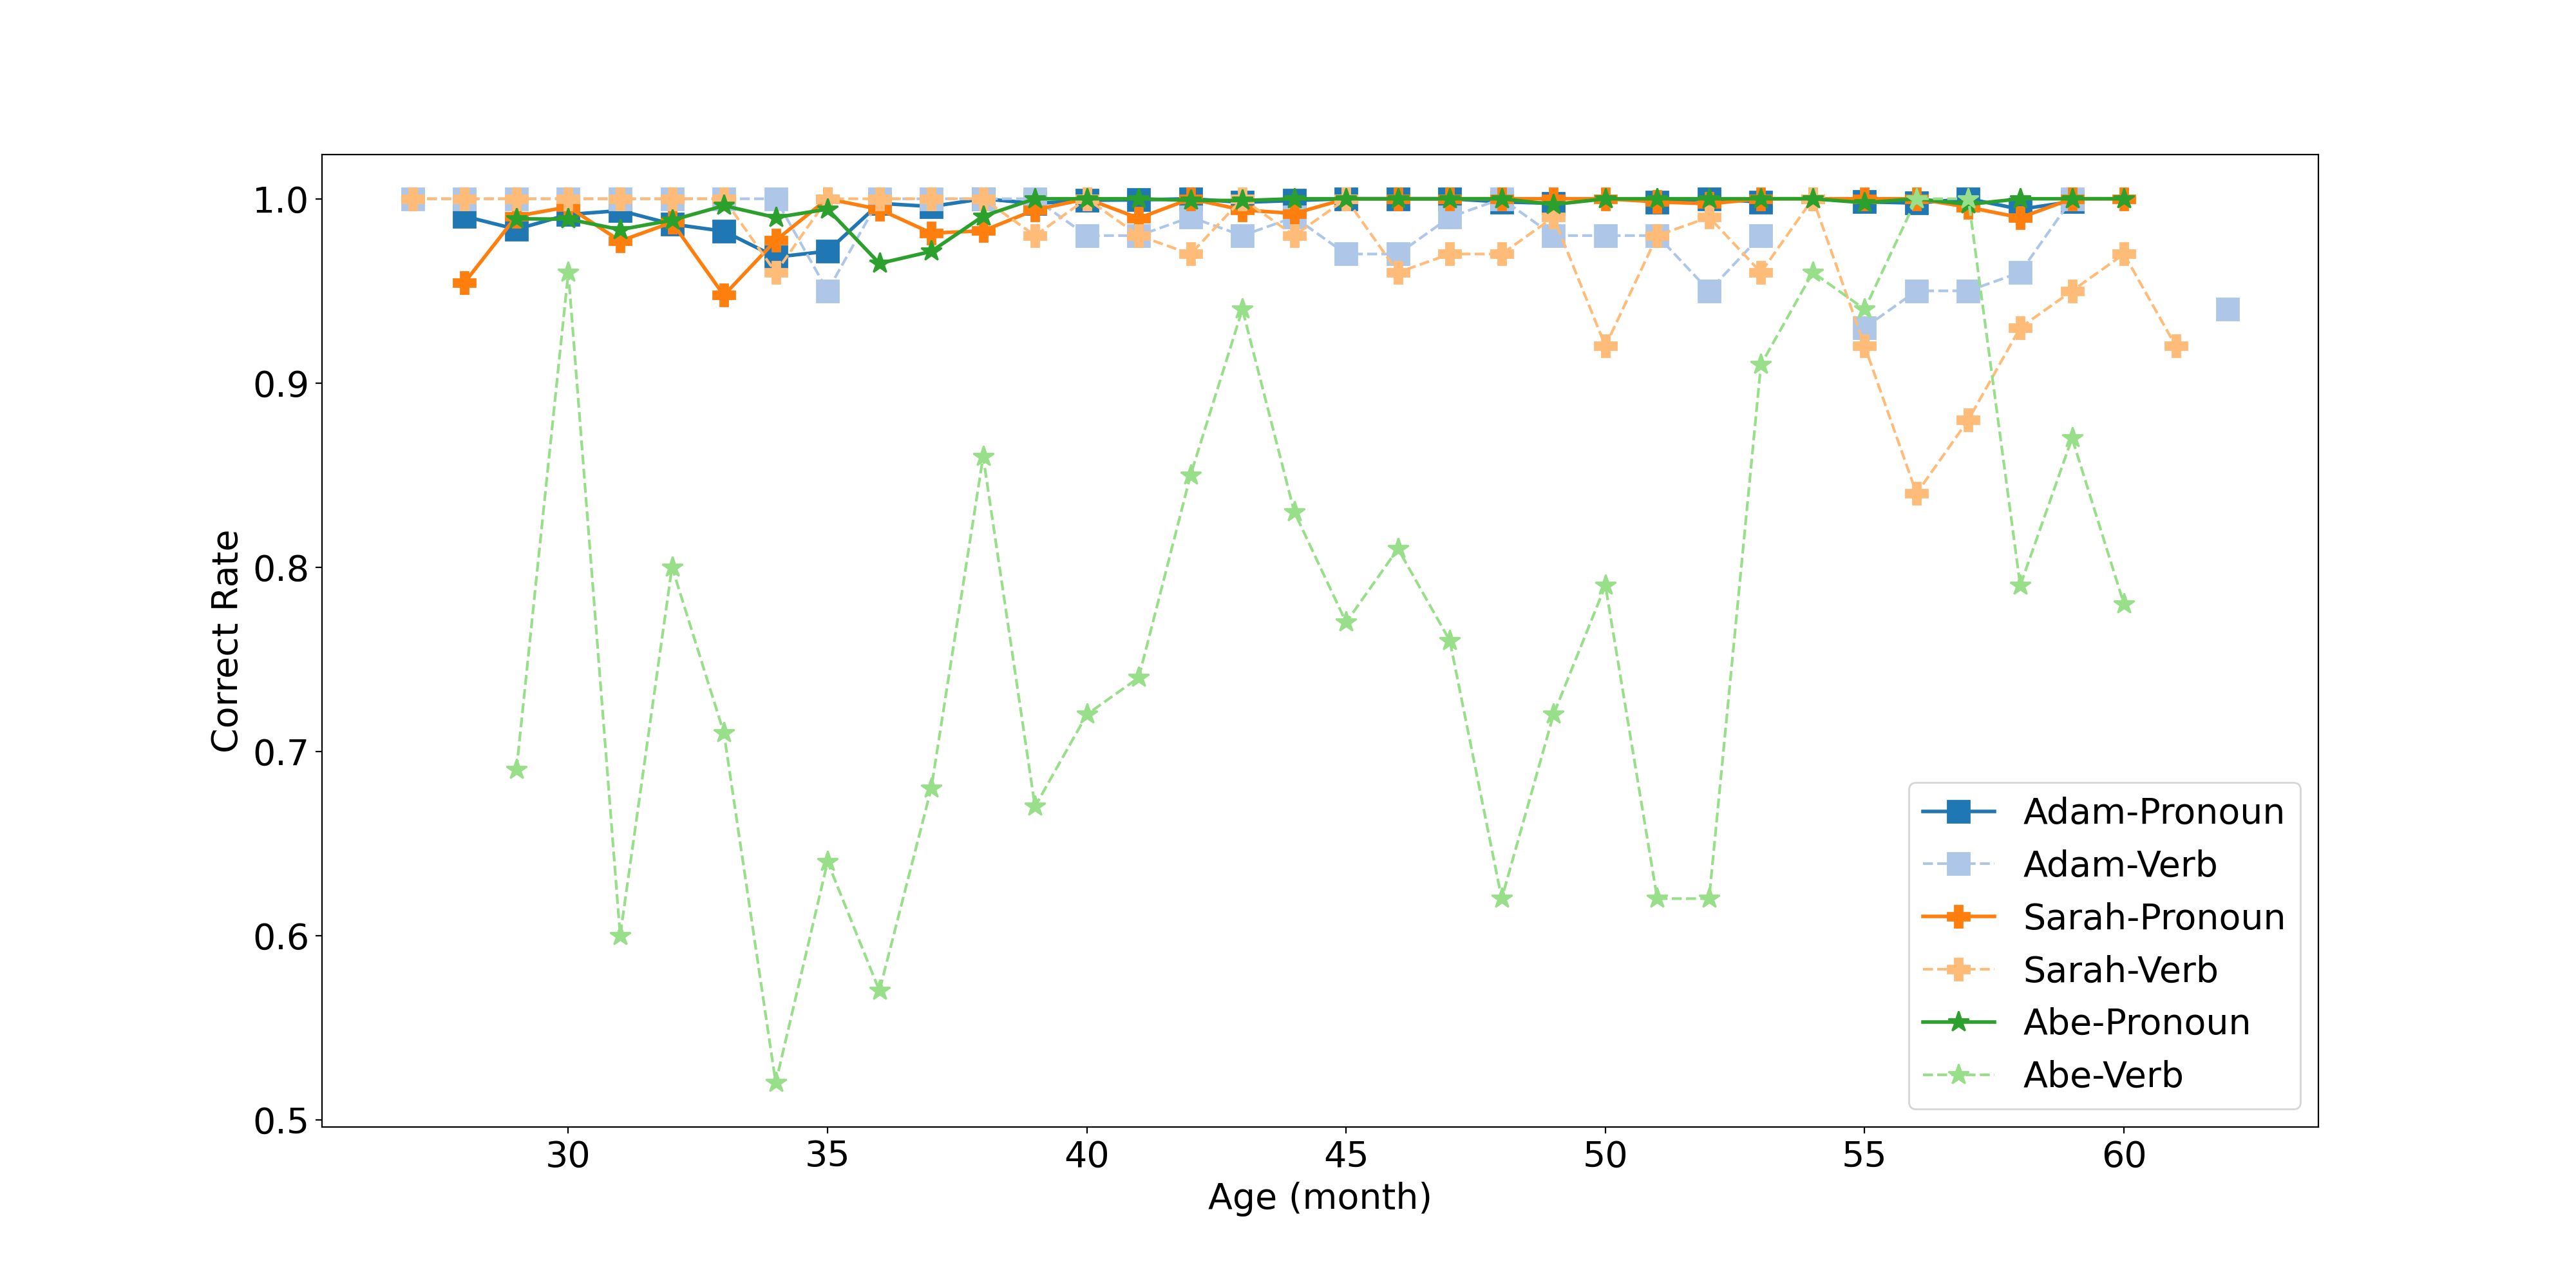
\includegraphics[scale = 0.35, width = \linewidth]{graph/AgeVerb.png}
\vspace{-3em}
\caption{Pronoun Correct Rate VS Verb Correct Rate for Adam, Abe and Sarah}
\label{fig:3}
\end{figure}
\FloatBarrier



\subsubsection{Different types of Pronoun Case Errors}
Children make many types of pronoun case errors as shown in previous sections. This subsection investigates the frequency of different types of pronoun case errors. The summary of pronoun case error data is shown in Table \ref{table:errordata}. 244,874 total pronouns were found in the children's longitudinal recordings. \textit{`I'},\textit{`my'} and \textit{`me'} are the most frequently used pronouns by the children; and \textit{`us'}, \textit{`their'} and \textit{`our'} are the least used pronouns. There were 3421 errors, with an average error rate of 1.39\%. There were five types of errors: nominative case used as an object (NOM for ACC), accusative case used as a subject (ACC for NOM) or a determiner (ACC for GEN), genitive case used as a subject (GEN for NOM) or an object (GEN for ACC). The most common errors occurred on pronoun \textit{`me'}, with 1579 \textit{`me'} used as \textit{`I'} and 165 \textit{`me'} used as \textit{`my'}. Seven pronouns (\textit{`I', `we', `she', `they', `his', `our'} and \textit{`their'}) have less than 10 errors. In addition, \textit{`I'} is the most commonly substituted pronoun, with 1579 \textit{`I's} being substituted by \textit{`me'} and 485 \textit{`I's} being substituted by \textit{`my'}, as shown in Column `Subs' in Table \ref{table:errordata}. `Pronoun Correct Rate by Use' in Column 6 is calculated as $1 - \displaystyle\frac{\text{Errors}}{\text{Total Tokens}}$.  For example, the correct rate by use for pronoun `I' is 1 -  $\displaystyle\frac{9}{118607} = 0.9999$. Most of the pronouns were used correctly over 95\% of the time, except for ‘me’ (91.80\%) and ‘her’ (91.14\%). `Pronoun Correct Rate by Argument Position' in Column 7 is calculated as the total argument positions (e.g. subject position, object position and determiner position) divided by the total positions that were  filled with a correct pronoun: $\displaystyle\frac{\text{Positions with correct pronoun}}{\text{Total argument positions}}$.  For example, for the subject position that requires a first person singular pronoun, the correct pronoun `\textit{I}' filled 118598 subject position, incorrect pronoun `\textit{me}' and `\textit{my}' filled 1579 and 485 subject positions respectively. Therefore, the correct rate by position for \textit{I} = $\displaystyle\frac{118607 - 9}{118607 - 9 + 1579 + 485} = 0.9829$. Most of the argument positions were filled with the correct pronoun over 98\% of the time, except for two positions: ‘she’ only filled 92.32\% of subject positions that required a third-person singular feminine pronoun and ‘their’ only filled 89.70\% of determiner positions that required a third-person plural pronoun. 

In addition, different types of errors are not equally popular among children. Children's errors are concentrated in three types of ACC for NOM errors: 41 children made `me-for-I' errors; 36 children made `them-for-they' errors and 30 children made `her-for-she' errors. Four types of errors (`she-for-her', `we-for-us', `they-for-them' and `our-for-we') had less than 5 children that made errors. Children don't make the same amount of errors on different error types. For some error types, children usually make that error once or twice. For example for `she-for-her' error, the maximum number of errors per child is 1 and there were 4 children who made such an error, meaning that each child only made the `she-for-her' error once. For other types of errors, there might be one or two children's errors accounted for a majority of the error tokens. For example, of total 1579 `me-for-I' errors, 858 errors were made by one child. 
 
\FloatBarrier
\begin{table}[h]
\footnotesize
\caption{Summary of Pronoun Case Error Data}
\label{table:errordata}
\begin{tabular}{c|cccccccc}
\hline
Pronoun & Tokens & Error Type & Errors & Subs & \begin{tabular}[c]{@{}l@{}}Pronoun\\ Correct\\ Rate by \\ Use\textsuperscript{a}\end{tabular} & \begin{tabular}[c]{@{}l@{}}Pronoun \\ Correct\\ Rate by\\ Argument\\ Position\textsuperscript{b}\end{tabular} & \begin{tabular}[c]{@{}l@{}}N children\\ making error\end{tabular} & \begin{tabular}[c]{@{}l@{}}Maximum\\ error/child\end{tabular} \\ \hline
I & 118607 & I-for-me & 9 & 2064 & 99.99\% & 98.29\% & 6 & 3 \\
he & 16966 & he-for-him & 27 & 157 & 99.84\% & 99.08\% & 14 & 8 \\
she & 4955 & she-for-her & 4 & 412 & 99.92\% & 92.32\% & 4 & 1 \\
we & 13525 & we-for-us & 4 & 14 & 99.97\% & 99.90\% & 3 & 2 \\
they & 9703 & they-for-them & 4 & 202 & 99.96\% & 97.96\% & 4 & 1 \\
me & 21280 & me-for-I & 1579 & 40 & \multirow{2}{*}{91.80\%} & \multirow{2}{*}{99.81\%} & 41 & 858 \\
 &  & me-for-my & 165 &  &  &  & 21 & 81 \\
him & 4732 & him-for-he & 148 & 27 & \multirow{2}{*}{95.79\%} & \multirow{2}{*}{99.24\%} & 26 & 26 \\
 &  & him-for-his & 51 &  &  &  & 11 & 30 \\
her & 4650 & her-for-she & 412 & 4 & 91.14\% & 99.94\% & 30 & 169 \\
us & 727 & us-for-we & 13 & 4 & 98.21\% & 99.73\% & 9 & 3 \\
them & 7181 & them-for-they & 194 & 4 & \multirow{2}{*}{95.95\%} & \multirow{2}{*}{99.94\%} & 36 & 42 \\
 &  & them-for-their & 97 &  &  &  & 23 & 17 \\
my & 35329 & my-for-I & 485 & 165 & \multirow{2}{*}{98.54\%} & 99.54\% & 25 & 124 \\
 &  & my-for-me & 31 &  &  &  & 7 & 8 \\
his & 5109 & his-for-he & 9 & 51 & 99.82\% & 99.01\% & 9 & 1 \\
our & 1265 & our-for-we & 1 & 0 & 99.92\% & 100.00\% & 1 & 1 \\
their & 845 & their-for-they & 8 & 97 & 99.05\% & 89.70\% & 6 & 2\\
\hline
\end{tabular}
\end{table}
\FloatBarrier

Why are children's pronoun case errors concentrated in few types of errors such as `\textit{me}-for-\textit{I}' and `\textit{her}-for-\textit{she}'? One possible explanation is that the error rate is related to how often children use a certain pronoun or how often children hear a certain pronoun in the parents' input. A Spearman's test shows that for each pronoun, there is a strong positive correlation between children's pronoun production and parents' pronoun input ($r_s$ = 0.80**, p <0.001), but there is no significant correlation between pronoun correct rate by use and children's pronoun production ($r_s$ = 0.22, p = 0.45) or parents' pronoun input ($r_s$ = 0.43, p = 0.13). Similarly, pronoun correct rate by position is not correlated with children's pronoun production ($r_s$ = -0.09, p = 0.77), or with parents' pronoun input ($r_s$ = -0.07, p = 0.81). Figure \ref{fig:corrct} visualizes that pronoun correct rate by rate and by position are not proportional to children's pronoun production or parents' input. In addition, each pronoun's error tokens are not correlated with children's pronoun production ($r_s$ = 0.30, p = 0.30) or with parents' pronoun input ($r_s$ = -0.01, p = 0.96). The results indicate that children do not produce more errors on a pronoun simply because they use that pronoun or hear that pronoun more often. Instead, children's pronoun production could be related to pronoun case errors in another way: the more often children use a pronoun, the more likely that pronoun is to be substituted. For example, \textit{`I'} is the most used pronoun by children. There were only 9 \textit{`I'}-for-\textit{'me'} errors, whereas 2064 \textit{`I'}s were substituted with \textit{`me'} and \textit{'my'}. A Spearman's test shows that children's pronoun production is positively correlated with pronouns' substituted tokens ($r_s$ = 0.56*, p = 0.03). The substituted tokens are not correlated with parents' pronoun input ($r_s$ = 0.47, p = 0.09). Figure \ref{fig:errortoken} shows that the error tokens are not correlated with children's and parents' pronoun tokens, and substituted tokens are correlated with children's pronoun production.


\FloatBarrier
\begin{figure}[!h]
    \centering
    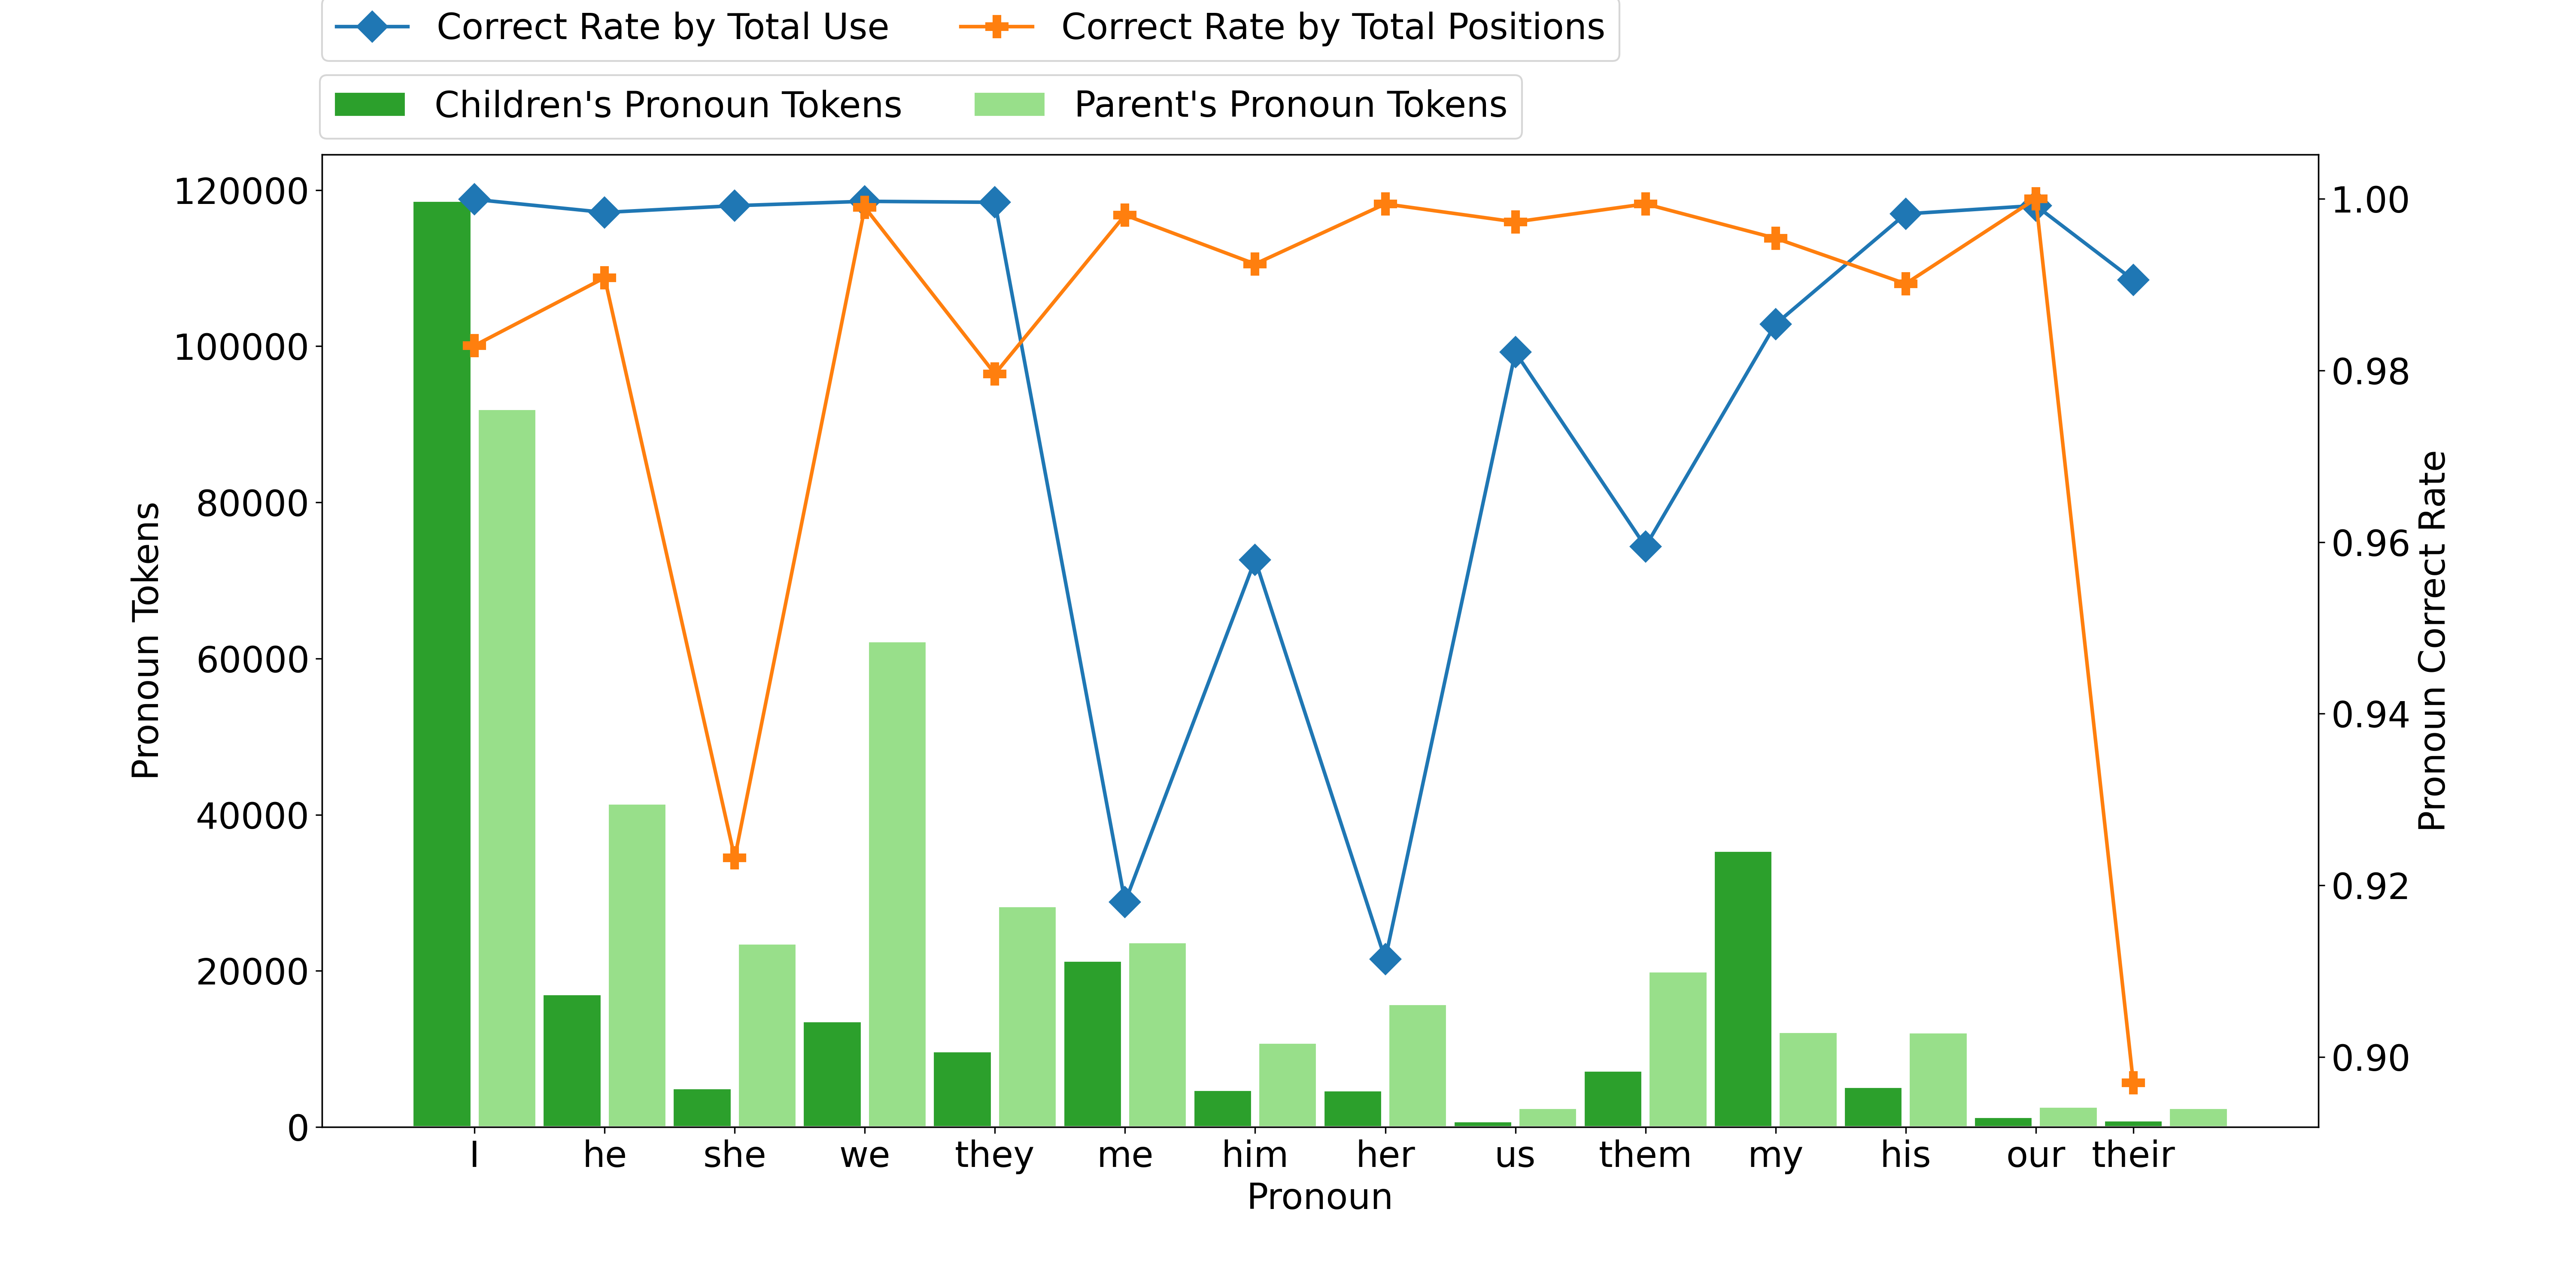
\includegraphics[scale = 0.35]{graph/PronounandRate.png}
    \vspace{-2em}
    \caption{Pronoun Correct Rate by Use and by Token, and Pronoun Tokens by Parents and Children }
    \label{fig:corrct}
\end{figure}
\FloatBarrier
\FloatBarrier
\begin{figure}[!h]
    \centering
    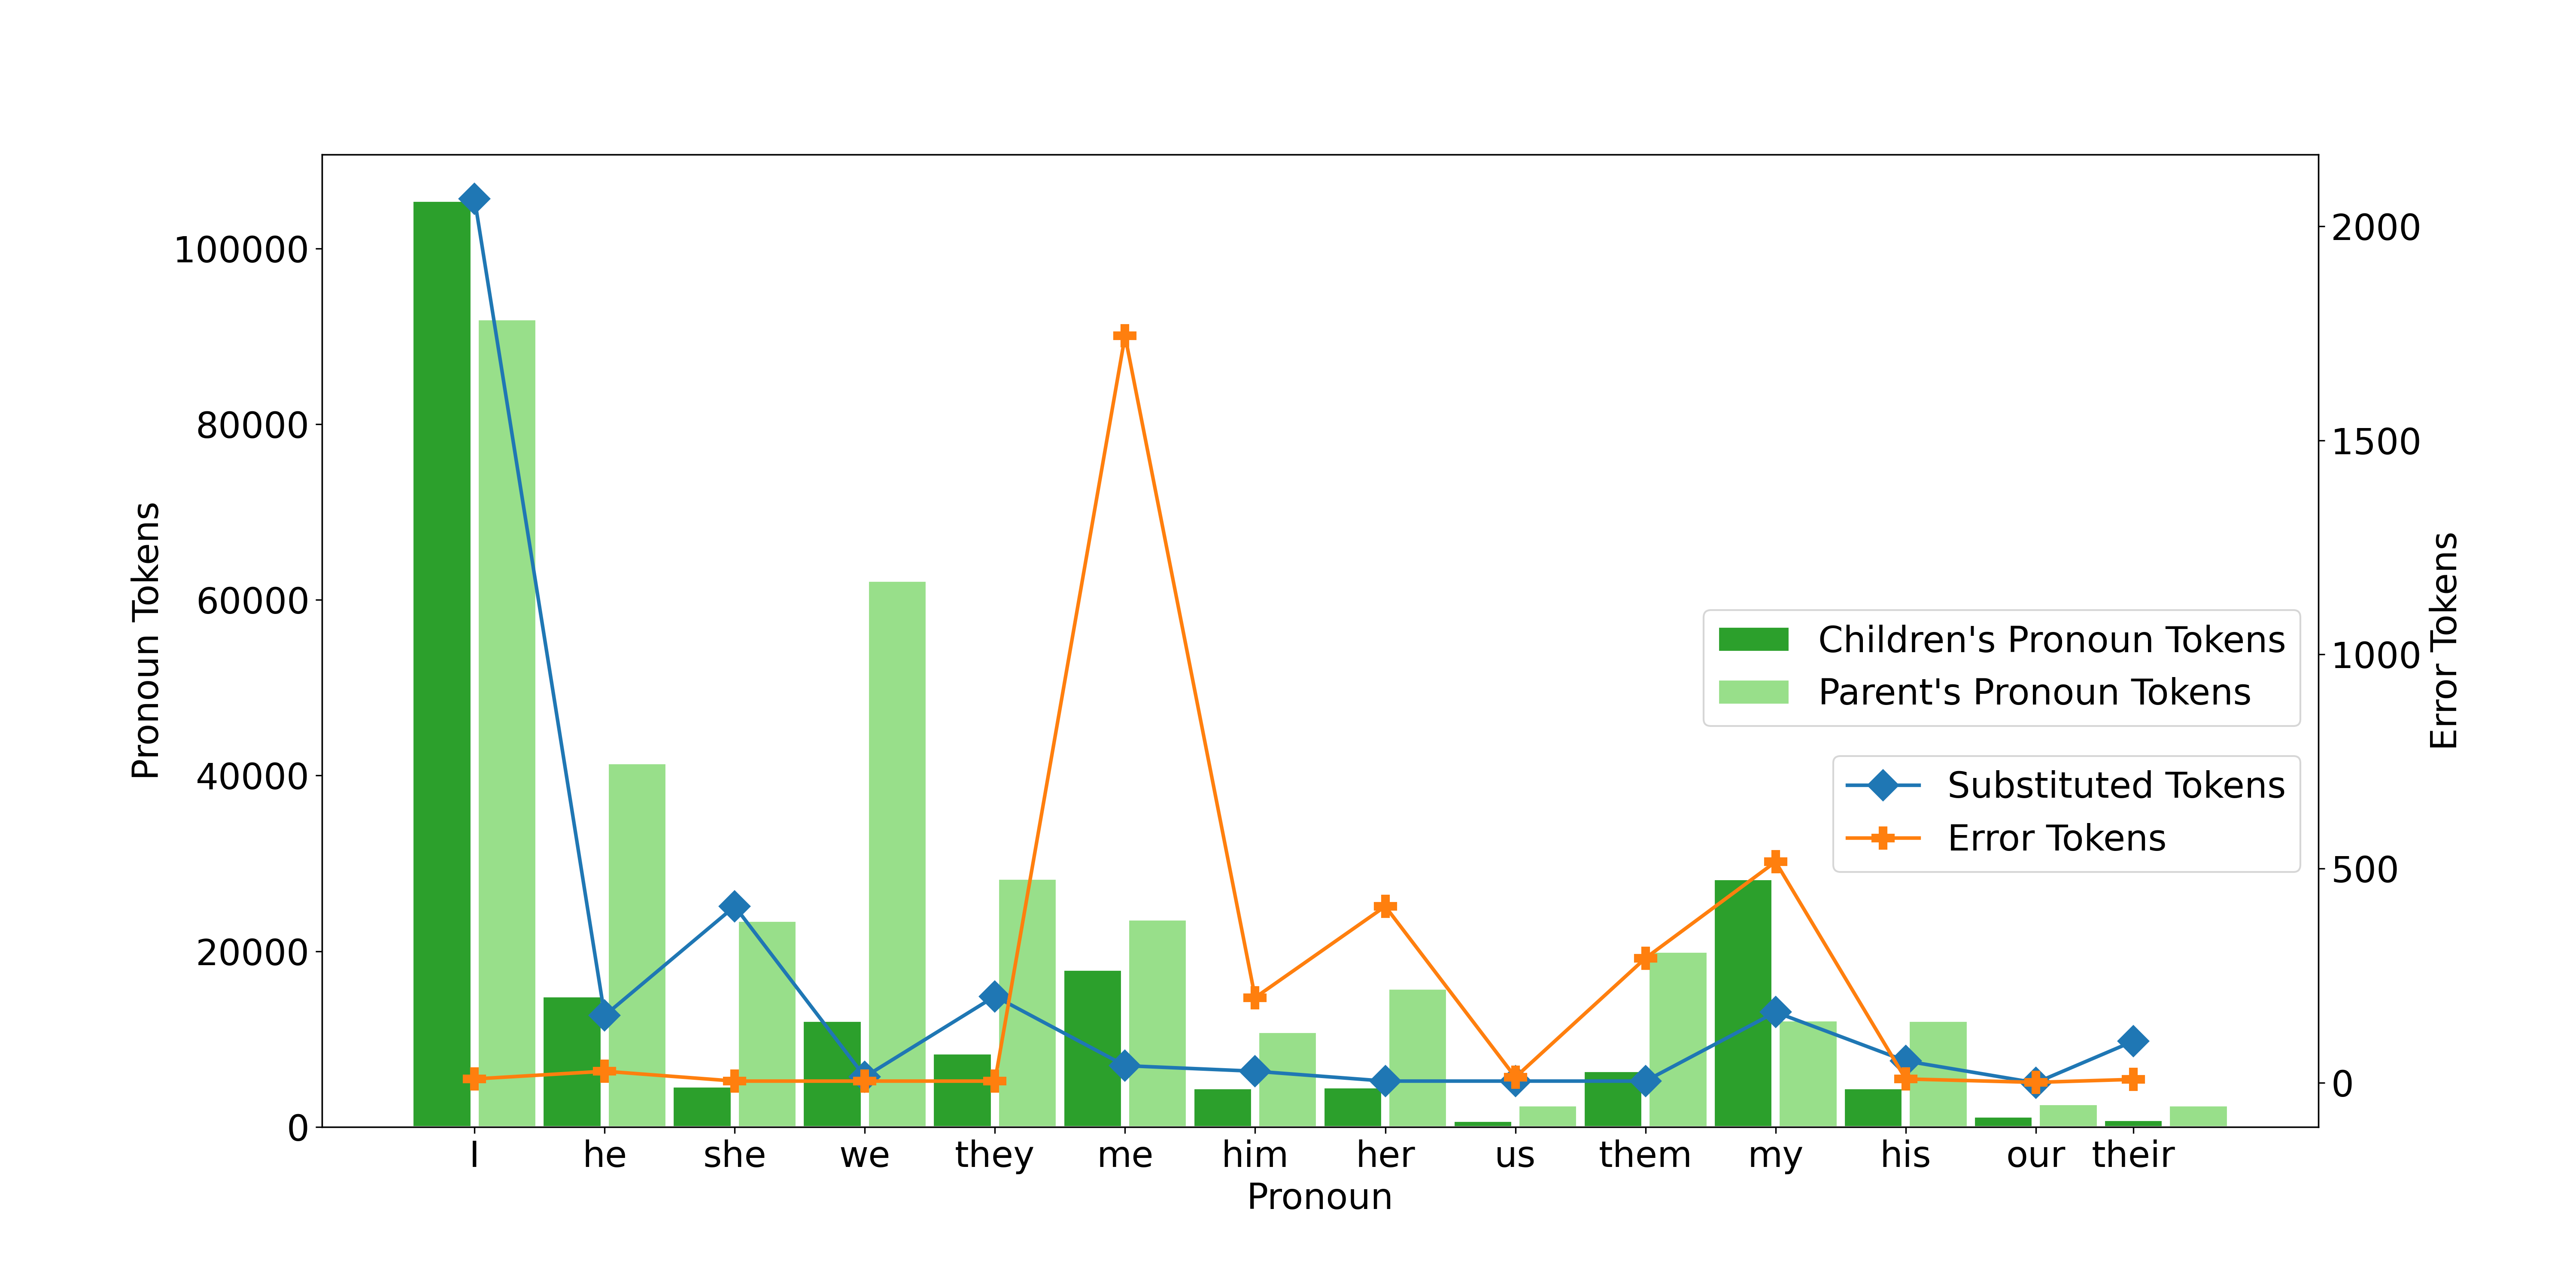
\includegraphics[scale = 0.35]{graph/Pronounandtoken.png}
    \vspace{-2em}
    \caption{Error tokens and Substituted tokens, and Pronoun tokens by Parents and Children}
    \label{fig:errortoken}
\end{figure}
\FloatBarrier


\subsection{Conclusion}
This section analyzed pronoun case errors' frequencies and patterns. First, pronoun case error is a relatively uncommon phenomenon, as most of the children rarely make any errors. 141 children in the cross-sectional data didn't make any errors, and 32 children with longitudinal recordings have less than a 1\% error rate. The average pronoun case error rate is also extremely low, with an average 1.16\% error rate for the cross-sectional data and 1.56\% for the longitudinal data. 

The pronoun case error rate has a non-monotonic relationship with children's age and mlu. The pronoun correct rate displays a U-shaped developmental pattern that children start with almost 100\% correct rate and decline to around 97\% and rise back to almost 100\% at around 5 years old. However, the correct rates at different age groups are not significantly different from each other. Since the error rate is so low during the U-shaped developmental sequences, it is difficult to judge if the changes in the correct rate are meaningful. 

Children's pronoun production and parents' pronoun input are not correlated with pronoun corrert rate or pronoun error tokens. The substituted tokens are correlated with children's pronoun production, suggesting that the more children use a pronoun, the more often that pronoun is replaced by an incorrect pronoun. 


\newpage
\section{Can Children's Verbal Use Explain Pronoun Case Errors? }
\subsection{Nominative case licensing}
The syntactic explanations focus on the non-nominative subject errors, where the accusative pronoun and the genitive pronoun are used as the subject (e.g. *\textit{me/my} eat it). In the syntactic theory, all structural cases are licensed by the head of a projection \citep[see][]{chomsky2000minimalist}. The nominative case is licensed by the \textsc{+finite} feature at the InflP level \citep[e.g.][]{haider1985unified, alec1991case} and the genitive case is licensed by the head of the DP \citep[e.g.][]{ritter1991two}. There are still debates about how the accusative case is assigned but it is agreed that it is assigned at the VP level or PP level. Other than structural cases, there is a default case in English, which is a case that doesn't denote grammatical relations or theta roles, but a filler when the case system failed to be checked. In English, the default case is the accusative case \citep{schutze1997, schutze2001}. For example, in sentences like `\textit{Who wants a cookie? - \textbf{Me}}', or `\textit{\textbf{Me} too}.' the accusative cased pronoun `me' is used as the default. Since the nominative case is licensed by the \textsc{+finite}, when a non-finite verb is used in a sentence, the system fails to check the nominative case. Thus the subject of the sentence will get the default case, which is the accusative case in English. For example, in the sentence `I went to school yesterday', the verb `went' is finite, thus the nominative case can be checked, resulting in `I' being the subject of the sentence. However, if the verb is non-finite in the sentence (e.g. the uninfected form of \textit{'went'}, '\textit{go}'), the nominative case won't get checked, resulting in the default accusative case used as the subject. Thus the sentence would be *`\textit{me} \textit{go} to school yesterday.' Young children often experience an Optional Infinitive stage \citep{wexler1994, wexler1998, wexler2000}, during which children would use non-finite verbs in their utterances. Although the theory doesn't explain why would children knowingly use the non-finite verb by omitting some verbal inflections, when the children use the non-finite verb, they would end up using the default accusative case as the subject, which leads to the non-nominative subject errors \citep{schutze1996subject, schutze1997}.  

The \textsc{+finite} feature in English can be realized in tense(\textsc{tns}), and/or person and number agreement (\textsc{arg}, e.g. third person singular agreement). The nominative case can be checked when any of the \textsc{+finite} features is present on the verbs, resulting in different configurations of the subject case and finite/non-finite verbs. Table \ref{tab: pattern} shows the predicted possible configuration of subject case and finiteness. 

\FloatBarrier
\begin{table}[!h]
    \centering
    \caption{The Configurations of finitenss with subject case (adapt from \cite{pine2005testing})}
    \begin{tabular}{llll}
    \toprule
        \textsc{Finiteness} & Case  & Examples  \\
    \hline
    Predicted to occur & & \\
         \textsc{+ arg, + tns} & \textsc{+ nom} & I am going. He goes. She's gone. She went.\\
         \textsc{- arg, - tns} & \textsc{- nom} & Me going. Him go. Her gone. Her went. \\
         (Omission of the inflections)\\
         \textsc{- arg, - tns} & \textsc{+nom} & I going. He goes. She's gone. \\
       \hline
       Predicted not to occur & & \\
       \textsc{+ arg, + tns} &  \textsc{-nom} & *\textit{Me am going. *Him goes. *Her's gone.} \\
        \bottomrule
    \end{tabular}
    \label{tab: pattern}
\end{table}
\FloatBarrier
In sum, the syntactic theory claims that the non-nominative subject error stems from the use of the non-finite verb. It predicts that when the verb is finite, the subject is almost never a non-nominative cased pronoun. 

\subsection{Testing the prediction}
The prediction was first tested on three children's data in CHILDES: Nina (1;11 - 2;5), Peter (1;11 - 2;5) and Sarah (2;8 - 3;1) \citep{schutze1996subject,schutze1997}. Only the pronoun subjects occurring with the unambiguous finite verbs and the unambiguous non-finite verbs were counted. The unambiguous finite verbs include auxiliaries, modals, copulas, past tense verbs, dummy \textit{do} and main verbs with \textit{-s}; and the unambiguous non-finite verbs include null auxiliary, null copula, main verbs and auxiliaries without \textit{-s}. Therefore, utterances like \textit{I go} or \textit{me go} are ignored. 
The tokens of nominative pronouns and non-nominative pronouns with finite verbs and non-finite verbs were tabulated and reproduced in Table \ref{table:schutzetotal} and Table \ref{tab:ATOMSchutze}. 
\FloatBarrier
\begin{table}[!h]
\centering
\caption{Total subject and verb form count for Nina, Peter, Sarah}
\label{table:schutzetotal}
\begin{tabular}{llll}
\toprule
 & \multicolumn{2}{l}{Verb Form} &\\ \cline{2-3} 
Subject & Finite & Non-Finite &\\ \hline
Nominative & 726  & 261  & 987 \\
Non-Nominative & 33  & 171  & 204 \\
\hline
& 759  & 432 & 1191  \\
\hline
 \multicolumn{4}{l}{Non-nominative finite rate = $\frac{33}{759}$ = 4.34\%} \\
\multicolumn{4}{l}{Finite non-nominative rate = $\frac{33}{204}$ = 16.18\%} \\
\bottomrule
\end{tabular}
\end{table}
\FloatBarrier

1191 subject pronouns were found that precede an unambiguous finite or non-finite verb in the corpus data of Nina, Peter and Sarah. Children generally use the subject correctly as 82.87\% of the subjects are nominative case. Children also use many non-finite verbs at this age, as only 63.73\% of the subjects precede a finite verb, fitting the description of the Optional Infinitival stage. Moreover, children have a strong tendency to use the nominative subjects with a finite verb. Of 759 pronoun subjects that precede a finite verb, only 33 of them are non-nominative pronouns, with an average non-nominative finite rate of 4.34\%. For different children and different pronouns, the non-nominative finite rate varies. For first person singular (1sg) pronoun, the rate is as low as 1.48\% for Peter and 3.08\% for Nina. For third person singular (3sg) pronouns, it was 7.09\% for Nina and 15.38\% for Sarah. The finite verbs following the non-nominative subjects are mostly past-tense verbs and modals, which only have \textsc{+tns} feature but not \textsc{+arg}. Therefore, \cite{schutze1997} concluded that `non-nominative subjects essentially never co-occur with agreeing verb forms'. In addition, \cite{schutze2001} further suggested that the non-nominative finite rate is so low that they can be regarded as noise in the data. 

However, the low non-nominative finite rate doesn't necessarily mean that non-nominative subjects almost never appear with a finite verb. First, there were too few data to confirm this finding: only three children's data were tested. Second, since children generally don't use that many non-nominative pronouns as the subject, there should be few non-nominative subjects that precede a finite verb. In addition, the non-nominative finite rate only calculates the percentage of non-nominative subjects of all the subjects precede a finite verb, which is not a fair representation of how often a non-nominative subject and a finite verb occur together. The percentage of the finite verbs of all verbs that follow a non-nominative pronoun should also be considered. Among 204 verbs that follow a non-nominative subject, 16.17\% of them are finite, which is not a low rate and shouldn't be counted as noise. The testing results in \cite{schutze1996subject} and \cite{schutze1997} only showed that when the non-nominative pronouns are used as subjects, the majority of them precede a non-finite verb, but didn't indicate that it's rare for them to precede a finite verb. 


\FloatBarrier
\begin{table}[!h]
    \caption{Reproducing \cite{schutze1997}'s data on Nina, Peter and Sarah}
    \label{tab:ATOMSchutze}
   \begin{minipage}[t]{0.5\textwidth}
    \centering
    \subcaption{Nina 1sg Finiteness VS Case}
    \small
    \begin{tabular}{@{}lll@{}}
        \toprule
         & \multicolumn{2}{c}{Verb form}\\
         \cline{2-3}
        Subject & Finite & Non-finite \\
        \midrule
        I & 189 & 63  \\
        me + my  & 6 & 18 \\
        \hline
         \multicolumn{3}{l}{Non-nominative finite rate = 3.08\%} \\
         \multicolumn{3}{l}{Finite non-nominative rate = 25\%}\\
        \bottomrule
    \end{tabular}
\end{minipage}
\vspace{1ex}
\begin{minipage}[t]{0.5\textwidth}
    \centering
    \subcaption{Nina 3sg Finiteness VS Case}
    \small
    \begin{tabular}{@{}lll@{}}
        \toprule
         & \multicolumn{2}{c}{Verb form}\\
         \cline{2-3}
        Subject & Finite & Non-Finite \\
        \midrule
        he + she & 249 & 149 \\
        him + her & 19 & 135 \\
        \hline
         \multicolumn{3}{l}{Non-nominative finite rate = 7.09\%} \\\multicolumn{3}{l}{Finite non-nominative rate = 12.33\%}\\
    \bottomrule
    \end{tabular}
    \end{minipage}
\vspace{1ex}
    %\caption{Nina Distribution by Verb Type}
    \begin{minipage}[t]{0.5\textwidth}
    \centering
    \subcaption{Nina 1sg Distribution by Verb Type}
    \small
    \begin{tabular}{lllll}
    \toprule
 &  & \multicolumn{3}{l}{Subject form} \\ \cline{3-5} 
Finiteness & Verb form & I & me & my \\ \hline
\multirow{2}{*}{\textsc{+arg}} & Auxiliary & 11 & 0 & 0 \\
 & Copula & 4 & 0 & 0 \\ \hline
\multirow{3}{*}{\textsc{+tns}} & Modal & 72 & 0 & 0 \\
 & Past Tense & 47 & 1 & 5 \\
 & Dummy \textit{do} & 55 & 0 & 0 \\ \hline
\multirow{2}{*}{\textsc{-finite}} & Null aux & 52 & 2 & 10 \\
 & Null cop & 11 & 2 & 4\\
\bottomrule
\end{tabular}
\end{minipage}
\vspace{1ex}
\begin{minipage}[t]{0.5\textwidth}
    \centering
    \subcaption{Nina 3sg Distribution by Verb Type}
    \small
\begin{tabular}{llllll}
\toprule
 &  & \multicolumn{4}{l}{Subject form} \\ \cline{3-6} 
Finiteness & Verb form & he & him & she & her \\ \hline
\multirow{3}{*}{\textsc{+arg}} & Main verb + \textit{`-s'} & 6 & 0 & 1 & 0 \\
 & Auxilliary + \textit{`-s'} & 113 & 0 & 3 & 3 \\
 & Copula + \textit{`-s'} & 88 & 3 & 2 & 4 \\ \hline
\multirow{2}{*}{\textsc{+tns}} & Modal & 13 & 1 & 1 & 2 \\
 & Past Tense & 20 & 0 & 2 & 6 \\ \hline
\multirow{4}{*}{\textsc{-finite}} & Main verb - \textit{`-s'} & 91 & 8 & 5 & 60 \\
 & Auxiliary - \textit{`-s'} & 19 & 0 & 1 & 14 \\
 & Null auxiliary & 24 & 1 & 0 & 27 \\
 & Null copula & 9 & 0 & 0 & 25\\
 \bottomrule
\end{tabular}
\end{minipage}
\vspace{1ex}
   \begin{minipage}[t]{0.5\textwidth}
    \centering
    \subcaption{Peter 1sg Finiteness VS Case}
    \small
    \begin{tabular}{@{}lll@{}}
        \toprule
         & \multicolumn{2}{c}{Verb form}\\
         \cline{2-3}
        Subject & Finite & Non-Finite \\
        \midrule
        I & 266 & 27 \\
        me + my  & 4 & 8\\
        \hline
         \multicolumn{3}{l}{Non-nominative finite rate = 1.48\%} \\
         \multicolumn{3}{l}{Finite non-nominative rate = 33.33\%}\\
        \bottomrule
    \end{tabular}
\end{minipage}
\vspace{1ex}
   \begin{minipage}[t]{0.5\textwidth}
    \centering
    \subcaption{Peter 1sg Distribution by Verb Type}
    \small
    \begin{tabular}{lllll}
    \toprule
 &  & \multicolumn{3}{l}{Subject form} \\ \cline{3-5} 
Finiteness & Verb form & I & me & my \\ \hline
\multirow{2}{*}{\textsc{+arg}} & Auxiliary & 126 & 0 & 0 \\
 & Copula & 10 & 0 & 0 \\ \hline
\multirow{3}{*}{\textsc{+tns}} & Modal & 54 & 0 & 0 \\
 & Past Tense & 74 & 3 & 1 \\
 & Dummy \textit{do} & 2 & 0 & 0 \\ \hline
\multirow{2}{*}{\textsc{-finite}} & Null aux & 27 & 4 & 2 \\
 & Null cop & 0 & 1 & 1\\
\bottomrule
\end{tabular}
\end{minipage}
\textbf{\linebreak}
\begin{minipage}[t]{0.5\textwidth}
    \centering
    \subcaption{Sarah 3sg Finiteness VS Case}
    \small
    \begin{tabular}{@{}lll@{}}
        \toprule
         & \multicolumn{2}{c}{Verb form}\\
         \cline{2-3}
        Subject & Finite & Non-Finite \\
        \midrule
        she & 22  & 22  \\
        her  & 4  & 10\\
        \hline
 \multicolumn{3}{l}{Non-nominative finite rate = 15.38\%} \\
\multicolumn{3}{l}{Finite non-nominative rate = 28.58\%}\\
        \bottomrule
    \end{tabular}
    \end{minipage}
\begin{minipage}[t]{0.5\textwidth}
    \centering
    \subcaption{Sarah 3sg Distribution by Verb Type}
    \small
 \begin{tabular}{llll}
\toprule
 &  & \multicolumn{2}{l}{Subject form} \\ \cline{3-4} 
Finiteness & Verb form & she & her \\ \hline
\multirow{3}{*}{\textsc{+arg}} & Main verb + \textit{`-s'} & 3 & 0 \\
 & Auxilliary + \textit{`-s'} & 6 & 0 \\
 & Copula + + \textit{`-s'} & 2 & 0 \\ \hline
\multirow{2}{*}{\textsc{+tns}} & Modal & 3 & 0 \\
 & Past Tense & 8 & 4 \\ \hline
\multirow{4}{*}{-finite} & Main verb - \textit{`-s'} & 9 & 7 \\
 & Auxiliary - \textit{`-s'} & 1 & 0 \\
 & Null auxiliary & 8 & 3 \\
 & Null copula & 4 & 0\\
 \bottomrule
\end{tabular}
\end{minipage}
\end{table}
\FloatBarrier

\cite{pine2005testing} proposed a straightforward way to test if the non-nominative subject almost never precedes a finite verb: by setting an upper limit as 10\%\footnote{They didn't explain the motivation to set the upper limite as 10\%.}, if the non-nominative finite rate is significantly larger than\footnote{A binomial test was used to compare the observed non-nominative rate and 10\%.} 10\%, then it is too frequent to be considered as noise. In their testing, they used a different criterion to select verb forms. Instead of using unambiguous finite and non-finite verbs, they used agreeing verbs and non-agreeing verbs. All the \textsc{+arg} verbs are considered as agreeing verbs, and the rest of the verbs are non-agreeing verbs, including \textsc{+tns} verbs, unambiguous non-finite verbs and ambiguous verbs. They first retested Nina's, Peter's and Sarah's data on 1sg pronoun and 3sg pronoun. Since there were no agreeing verbs that precede \textit{me} and \textit{my} in Nina's and Peter's data, they focused on the non-nominative rate of 3sg pronoun in Sarah's and Nina's data. Sarah didn't use any \textit{him} or \textit{her} that precede an agreeing verb either. For Nina, 4.48\% of the 3sg subjects that precede an agreeing verb are non-nominative pronouns, which is significantly smaller than 10\%. However, the masculine and feminine pronouns behave differently. The non-nominative pronoun \textit{her} takes 53.85\% of the 3sg feminine subjects with a finite verb, which is significantly greater than 10\%. The re-test result for Nina's 3sg subjects is reproduced in Table \ref{table:nina}.
\FloatBarrier
\begin{table}[!h]
\centering
\caption{Distribution of Nina's 3sg pronoun subject's case and agreeing verbs from in \cite{pine2005testing}}
\label{table:nina}
\begin{tabular}{lll}
\toprule
 & \multicolumn{2}{l}{Verb Form} \\ \cline{2-3} 
Subject & Agreeing & \begin{tabular}[c]{@{}l@{}}Non-\\ Agreeing\end{tabular} \\ \hline
He + She & 213 & 185 \\
Him/His + Her & 10 & 144 \\ \hline
\multicolumn{3}{l}{Non-nominative finite rate = $\frac{10}{213+10}$ = 4.48\%} \\ \hline
She & 6 & 9 \\
Her & 7 & 134 \\ \hline
\multicolumn{3}{l}{Non-nominative finite rate = $\frac{7}{6+7}$ = 53.85\%*}\\
\bottomrule
\end{tabular}
\end{table}

\FloatBarrier

In addition, they did the same test on four more children: Anne, Becky and Gail, from the Manchester corpus \citep{theakston2001} and Abe from  \cite{kuczaj1977acquisition}, who produced enough non-nominative 3sg subjects with agreeing verbs that can be properly tested. The average non-nominative finite rate for 3sg pronoun is 7.08\%, which is not significantly greater than 10\%. However, the rate for 3sg feminine pronoun is 43.01\%, which is significantly greater than 10\%.  The results are reproduced in Table \ref{tab:fourtotal}. 
\FloatBarrier
\begin{table}[!h]
\centering
\caption{Distribution of 3sg pronoun subject's case and agreeing verb forms for Anne, Becky, Gail and Abe}
\label{tab:fourtotal}
\begin{tabular}{lll}
\toprule
 & \multicolumn{2}{l}{Verb Form} \\ \cline{2-3} 
Subject & Agreeing & \begin{tabular}[c]{@{}l@{}}Non-\\ Agreeing\end{tabular} \\ \hline
He + She & 629 & 305 \\
Him/His + Her & 48 & 59 \\ \hline
\multicolumn{3}{l}{Non-nominative finite rate = $\frac{48}{629+48}$ = 7.08\%} \\ \hline
She & 53 & 41 \\
Her & 40 & 47 \\ \hline
\multicolumn{3}{l}{Non-nominative finite rate = $\frac{40}{53+40}$ = 43.0\%*}\\
\bottomrule
\end{tabular}
\end{table}
\FloatBarrier
This pattern is also true for each individual child. All four children's total 3sg non-nominative finite rate is significantly less than or no different from 10\%, but 3sg feminine non-nominative subject `her' consistently precedes a finite verb over 10\% of the time. The distribution of subject case and agreeing verbs for each child is reproduced in Table \ref{tab: Pine}.
\FloatBarrier
\begin{table}[!h]
\centering
\caption{Each child's distribution of 3sg pronoun subject's case and agreeing verb forms from \cite{pine2005testing}}
\label{tab: Pine}
\begin{tabular}{llll|lll}
\toprule
 &  & Agreeing & \begin{tabular}[c]{@{}l@{}}Non-\\ Agreeing\end{tabular} &  & Agreeing & \begin{tabular}[c]{@{}l@{}}Non-\\ Agreeing\end{tabular} \\ \hline
\multirow{3}{*}{Anne} & He+She & 131 & 73 & She & 8 & 11 \\
 & Him/His + Her & 5 & 6 & Her & 4 & 3 \\ \cline{2-7} 
 & \multicolumn{3}{l|}{Non-nominative finite rate = 3.4\%} & \multicolumn{3}{l}{Non-nominative finite rate = 33.3\%*} \\ \hline
\multirow{3}{*}{Becky} & He+She & 239 & 80 & She & 26 & 22 \\
 & Him/His + Her & 16 & 2 & Her & 13 & 0 \\ \cline{2-7} 
 & \multicolumn{3}{l|}{Non-nominative finite rate =  6.3\%} & \multicolumn{3}{l}{Non-nominative finite rate = 33.3\%*} \\ \hline
\multirow{3}{*}{Gail} & He+She & 146 & 48 & She & 14 & 3 \\
 & Him/His + Her & 13 & 16 & Her & 9 & 10 \\ \cline{2-7} 
 & \multicolumn{3}{l|}{Non-nominative finite rate =  8.2\%} & \multicolumn{3}{l}{Non-nominative finite rate = 39.1\%*} \\ \hline
\multirow{3}{*}{Abe} & He+She & 113 & 104 & She & 5 & 5 \\
 & Him/His + Her & 14 & 35 & Her & 14 & 34 \\ \cline{2-7} 
 & \multicolumn{3}{l|}{Non-nominative finite rate = 11.0\%} & \multicolumn{3}{l}{Non-nominative finite rate = 73.7\%*}\\
 \bottomrule
\end{tabular}
\end{table}
\FloatBarrier
Thus, \cite{pine2005testing} concluded that it is not true that the non-nominative subjects almost never precede a finite verb. For 3sg feminine pronoun, the non-nominative form \textit{her} appears with a finite verb quite frequently and of all the 3sg feminine subjects that precede a finite verb 43\% of them are \textit{her}. The data doesn't support the prediction of the syntactic explanation that the non-nominative subject almost never occurs with a finite verb. In addition, children generally don't use many non-nominative pronouns as the subject, and there are even less of them that precede a finite verb, which makes the syntactic prediction particularly difficult to test. 

\subsection{Re-testing the prediction}
The syntactic explanation claims that the use of the non-finite verb is the reason for the non-nominative subject. It predicts that there should be no non-nominative subjects preceding a finite verb; and if there are any in the children's data, those are just noise. In different children's corpus data, the average non-nominative finite rate for the 1sg and the 3sg pronouns is significantly lower than 10\%, which some argue that could be treated as noise. However, the 3sg feminine pronoun's non-nominative finite rate is significantly larger than 10\%, which contradicts the prediction. This section reviews the existing testing methods and argues that the non-nominative finite rate should not be judged by its surface value. The low rate doesn't necessarily mean that the non-nominative subjects rarely precede a finite verb.

In \cite{schutze1996subject} and \cite{pine2005testing}, the non-nominative finite rate is calculated as the number of non-nominative subjects preceding a finite verb over the total subject pronouns that precede a finite verb, or cell `c' over the sum of cell `a' and `c' in the 2x2 contingency table in Table \ref{tab:2x2}. 

\begin{equation}
\label{equ:1}
\centering
     \text{non-nominative finite rate} = \displaystyle\frac{\text{non-nominative finite subjects }}{\text{total finite pronoun subjects}} = \displaystyle\frac{\text{c}}{\text{a+c}}
\end{equation}

\FloatBarrier
\begin{table}[!h]
\centering
\caption{2x2 Contingency Table of subject case and verb form}
\label{tab:2x2}
\begin{tabular}{lll}
\toprule
 & \multicolumn{2}{l}{Verb Form} \\ \cline{2-3} 
 & Finite & Non-finite \\
Nominative & a & b \\
Non-nominative & c & d\\
\bottomrule
\end{tabular}
\end{table}
\FloatBarrier

The non-nominative finite rate calculated in Equation \ref{equ:1}  actually is the conditional probability of a  non-nominative subject given a finite verb: 
\begin{align*}
\label{equ:44}
\centering
\text{non-nominative finite rate} & = \text{P(Non-nominative|Finite)}\\
&= \displaystyle\frac{\text{P(Non-nominative $\cap$ Finite)}}{\text{P(Finite)}}\\
& = \displaystyle\frac{\displaystyle\frac{\text{c}}{\text{a+b+c+d}}}{\displaystyle\frac{\text{a+c}}{\text{a+b+c+d}}} = \displaystyle\frac{\text{c}}{\text{a+c}}
\end{align*}
Therefore, the surface value of the rate doesn't truly reflect if a non-nominative subject never occurs with a finite verb. In order to decide whether the presence of a finite verb blocks the use of a non-nominative subject, the rate needs to be compared to the probability of non-nominative subject P(Non-nominative). If P(Nominative) and P(Finite) are independent events, meaning that the presence of finite verb does not affect the use of non-nominative subjects, the conditional probability P(Non-nominative|Finite) equals P(Non-nominative): 
\begin{align*}
   \text{P(Non-nominative|Finite)} &= 
   \displaystyle\frac{\text{P(Non-nominative $\cap$ Finite)}}{\text{P(Finite)}}\\
   &= \displaystyle\frac{\text{P(Non-nominative) $\times$ P(Finite)}}{\text{P(Finite)}}\\
   &= \text{P(Non-nominative)}\\
   &= \displaystyle\frac{\text{c+d}}{\text{a+b+c+d}}
\end{align*}
If P(Non-nominative|Finite)is significantly smaller than P(Non-nominative), it means that P(Non-nominative) and P(Finite) are not independent, indicating that the presence of the finite verb prevents the non-nominative subjects. For example, assume that P(Non-nominative) is only 5\%, if  P(Non-nominative|Finite) is 1\%, which is even smaller than 5\%, then it is even more unlikely to see a non-nominative subject when there is a finite verb. However, if P(Non-nominative|Finite) is 8\%, it suggests that the presence of the finite verb actually increases the probability of a non-nominative subject, although 8\% is a relatively low rate.  

Therefore, the P(Non-nominative|Finite) ($\displaystyle\frac{\text{c}}{\text{a+c}}$) should be compared to P(Non-nominative) ($\displaystyle\frac{\text{c+d}}{\text{a+b+c+d}}$), and if it is significantly smaller than P(Non-nominative), it can be concluded that the non-nominative subject almost never appears before a finite verb. The log-likelihood ratio test (the \textit{G}-test) was used to compare P(Non-nominative|Finite) and P(Non-nominative). The G-statistic can be calculated as the natural log of the observed number (\textit{O}) divided by the expected number (\textit{E}) and multiply by 2. The formula for G is:
\begin{equation}
    \centering
    G = 2 \times \displaystyle\sum_{i = 1}^{n}(O_i \times ln(\displaystyle\frac{\text{$O_i$}}{\text{$E_i$}}))
\end{equation}

The observed numbers are the number of nominative and non-nominative subjects preceding a finite verb, which are cell `a' and cell `c' in the 2x2 contingency table, as shown in Table \ref{tab:tada}. The expected numbers are the pronoun subjects preceding a finite verb assuming that P(Non-nominative) and P(Finite) are independent. The expected number of nominative finite subjects ($E_{Nominative}$) and expected non-nominative finite subjects ($E_{Non-nominative}$) is calculated as the total numbers of subjects precede a finite verb times P(Nominative|Finite) and P(Non-nominative|Finite):
\begin{align*}
    E_{Nominative} & = \text{(a+c)} \times \text{P(Nominative|Finite)} \\
    & = \text{(a+c)} \times \text{P(Nominative)} \\
    & = \text{(a+c)} \times \displaystyle\frac{\text{a+b}}{\text{a+b+c+d}}\\
    & = \displaystyle\frac{\text{(a+c)(a+b)}}{\text{a+b+c+d}}
\end{align*}
\begin{align*}
    E_{Non-nominative} & = \text{(a+c)} \times \text{P(Non-nominative|Finite)} \\
    & = \text{(a+c)} \times \text{P(Non-nominative)} \\
    & = \text{(a+c)} \times \displaystyle\frac{\text{c+d}}{\text{a+b+c+d}} \\
     & = \displaystyle\frac{\text{(a+c)(c+d)}}{\text{a+b+c+d}}
\end{align*}
\FloatBarrier
\begin{table}[!h]
\centering
\caption{Observed and Expected numbers and P(Non-nominative) and \text{r\%} represented by cell numbers in 2x2 contingency table}
\label{tab:tada}
\begin{tabular}{llll}
\toprule
 & \begin{tabular}[c]{@{}l@{}}Total Pronoun  \\
Subjects\end{tabular} &\begin{tabular}[c]{@{}l@{}}Observed \\
 Agreeing Subjects\end{tabular} & \begin{tabular}[c]{@{}l@{}}Expected \\ Agreeing Subjects\end{tabular} \\ 
 \hline 
Nominative & a+b & a & \displaystyle\frac{\text{(a+c)(a+b)}}{\text{a+b+c+d}} \\[1.5ex]
\hline 
Non-nominative & c+d & c & \displaystyle\frac{\text{(a+c)(c+d)}}{\text{a+b+c+d}} \\ [1.5ex]
\hline
\multicolumn{4}{l}{P(Non-nominative) = \displaystyle\frac{\text{c+d}}{\text{a+b+c+d}}, \text{P(Non-nominative|Finite)} = \displaystyle\frac{\text{c}}{\text{a+c}}}\\
\bottomrule
\end{tabular}
\end{table}
\FloatBarrier


The data reported in \cite{schutze1997} and \cite{pine2005testing} were used to calculated the G-statistics of P(Non-nominative) and P(Non-nominative|Finite) in 1sg pronouns and 3sg pronouns. Following \cite{pine2005testing}, finite verbs were counted as agreeing verbs. The test result of 1sg pronouns is shown in Table \ref{Tab:gtest1}\footnote{The counts are different from Table \ref{tab:ATOMSchutze} because different verb selection criteria were applied. In Table \ref{tab:ATOMSchutze}, finite forms only included the unambiguous \textsc{+tns} and/or \textsc{+arg} verbs, and non-finite forms only included the unambiguous non-finite verbs. In Table \ref{Tab:gtest1}, only agreeing verbs were counted as finite verbs.}. Both Nina's P(Non-nominative|Finite) (3.07\%) and Peter's P(Non-nominative|Finite) (1.48\%) are significantly smaller than their P(Non-nominative), suggesting that the non-nominative first person pronoun (\textit{me} and \textit{my}) rarely precedes a non-finite verb. 

\FloatBarrier
\begin{table}[!h]
\centering
\caption{G-test for 1sg pronoun for Nina and Peter (data reproduced from \cite{schutze1997})}
\label{Tab:gtest1}
\begin{tabular}{lllll}
\toprule
 & & \begin{tabular}[c]{@{}l@{}}Total Pronoun \\ Subjects\end{tabular} & \begin{tabular}[c]{@{}l@{}}Observed \\ Agreeing Subjects\end{tabular} & \begin{tabular}[c]{@{}l@{}}Expected \\ Agreeing Subjects\end{tabular} \\ \hline
\multirow{3}{*}{Nina} & I & 903 & 189 & 169.31 \\ \cline{2-5} 
 & me + my & 137 & 6 & 25.68 \\ \cline{2-5} 
 & & \multicolumn{3}{l}{P(Non-nominative)\% = 13.17\%, P(Non-nominative|Finite)\% = 3.07\%}\\
 & &\multicolumn{3}{l}{\textbf{G = 24.13***}, p <0.001} \\ \hline
\multirow{3}{*}{Peter} & I & 700 & 266 & 243.56 \\ 
\cline{2-5}
 & me + my & 76 & 4 & 26.44 \\ \cline{2-5} 
 & & \multicolumn{3}{l}{P(Non-nominative)\% = 9.79\%, P(Non-nominative|Finite)\% =1.48\%}\\
 &&\multicolumn{3}{l}{\textbf{G = 31.78***}, p<0.001} \\
 \bottomrule
\end{tabular}
\end{table}
\FloatBarrier

In addition, more children's 1sg data were added to test for the G-statistics. The selection criteria include: (1) the children have to produce enough non-nominative subject errors, which means P(Non-nominative) $\geq$ 2\%; (2) the children have to produce more than 2 non-nominative subjects that precede a finite verb, which means cell `c' $\geq$ 2. Only seven more children fit the selection criteria: Ruth, Nicole, Warren and Anne from the Manchester corpus \citep{theakston2001}, Laura from \cite{braunwald1971mother}, Eve from Brown corpus \citep{brown1973first} and Naomi from \cite{sachs1983talking}. The G-test results for the seven more children are shown in Table \ref{tab:7more}. Only three children's P(Non-nominative|Finite) is significantly smaller than P(Non-nominative): Ruth's 48.68\% < 60.04\%; Warren's 2.62\% < 6.56\% and Anne's 1.42\% < 3.19\%. For the other four children, their 1sg pronoun's  P(Non-nominative|Finite) is not significantly smaller than P(Non-nominative), indicating that the presence of a finite verb doesn't prevent \textit{me} and \textit{my} being used as the subject.  

The results of 3sg masculine and feminine pronouns are shown in Tables \ref{tab:himhigtest} and \ref{tab:hershegtest}. Although 3sg masculine pronoun's P(Non-nominative|Finite) is extremely low for all four children, ranging from 2.94\% to 0.75\%, none of the P(Non-nominative|Finite) is significantly smaller than P(Non-nominative), indicating that the finite verb doesn't prevent the non-nominative pronouns \textit{him} and \textit{his} from preceding an agreeing verb. The 3sg feminine pronoun's P(Non-nominative) are all relatively high for all five children, ranging from 33.33\% to 73.68\%. For Anne and Becky, their P(Non-nominative|Finite) (33.33\% for both) are even larger than their P(Non-nominative) (26.92\% and 21.31\% respectively). However, none of the P(Non-nominative) is significantly different from P(Non-nominative|Finite), except for Nina. Nina mostly used \textit{her} as a subject; she has the highest P(Non-nominative), which is 90.38\%, but her P(Non-nominative|Finite) is 62.5\%, which is significantly smaller than P(Non-nominative). The G-test results demonstrate that it is not rare for \textit{her} as a subject to precede a finite verb.

In addition, all children's 1sg and 3sg pronouns' P(Non-nominative) and P(Non-nominative|Finite) were combined for a meta-analysis. Table \ref{tab: Pnon} shows each child's P(Non-nominative) and P(Non-nomiantive|Finite)\footnote{For Nina and Anne, the non-nominative pronouns include the total counts of 1sg \textit{me/my}and 3sg pronouns \textit{him/his} and \textit{her}. For Becky and Gail, the non-nominative pronouns included the total counts of 3sg pronouns \textit{him/his} and \textit{her}.}. An exact sign test shows that the median difference in P(Non-nominative) and P(Non-nominative|Finite) is significant (p = 0.004), meaning that the presence of a finite verb decreases the possibility of a non-nominative pronoun being used as a subject by 2.81\%. 

\FloatBarrier
\begin{table}[h]
\centering
\caption{12 Children's P(Non-nominative) and P(Non-nomiantive|Finite)}
\label{tab: Pnon}
\begin{tabular}{l|cc}
\toprule
 & P(Non-nominative) & P(Non-nominative|Finite) \\
 \hline
Peter & 9.79\% & 1.48\% \\
Ruth & 60.04\% & 48.68\% \\
Nicole & 5.35\% & 3.68\% \\
Warren & 6.56\% & 2.62\% \\
Laura & 2.22\% & 2.06\% \\
Eve & 2.03\% & 1.95\% \\
Naomi & 2.10\% & 1.20\% \\
Abe & 82.76\% & 73.68\% \\
Nina & 18.19\% & 5.40\% \\
Anne & 3.5\% & 2.01\% \\
Becky & 5.34\% & 6.27\% \\
Gail & 13\% & 8.18\% \\
\hline
median & 5.96\% & 3.15\%\\
\bottomrule
\end{tabular}
\end{table}
\FloatBarrier
In addition, in order to test if the P(Non-nominative|Finite) is smaller than P(Non-nominative) for 1sg, 3sg masculine and 3sg feminine pronouns, the p-values of children's G-test were combined using Fisher's method. The formula is shown in Equation \ref{equ3}, where p_i is the p-value for each G-test, k is the number of tests being combined. $\chi^2$ has a chi-squared distribution with $2k$ degrees of freedom.
\begin{equation}
\label{equ3}
    \chi^2_{2k} \sim -2\displaystyle\sum^k_{i=1}ln(p_i)
\end{equation}
For 9 children with 1sg pronoun's data, the $\chi^2$ is 101.7. The critical value (p<0.05) of chi-square for df = 18 is 28.87, indicating that P(\textit{me+my }|Finite) is significantly smaller than P(\textit{me+my}). For 5 children with 3sg feminine pronoun's data, the $\chi^2$ is 28.12. The critical value (p<0.05) of chi-square for df = 10 is 18.31, suggesting that P(\textit{her }|Finite) is significantly smaller than P(\textit{her}). For 4 children with 3sg masculine pronoun's data, the $\chi^2$ is 11.52. The critical value (p<0.05) of chi-square for df = 8 is 15.51, showing that P(\textit{him+his }|Finite) is not significantly different from P(\textit{him+his}). 


In conclusion, the meta-analysis shows that P(Non-nominative|Finite) is generally significantly smaller than P(Non-nominative), suggesting that the finite verb could decrease the possibility of a non-nominative pronoun being used as the subject. However, there is great variance among different children and different pronouns. For 1sg pronoun, 4 out of 9 children's P(\textit{me+my}) is not significantly different from P(\textit{me+my}|Finite). For 3sg masculine pronoun, all 4 children's P(\textit{him+his}|Finite) is not different from P(\textit{him+his}). For 3sg feminine pronoun, 4 out of 5 children's P(\textit{her}) is not different from P(\textit{her}|Finite). 

\FloatBarrier
\begin{table}[!h]
\centering
\caption{G-test of 1sg pronoun for seven more children}
\label{tab:7more}
\begin{tabular}{lllll}
\toprule
 &  & \begin{tabular}[c]{@{}l@{}}Total Pronoun\\ Subjects\end{tabular} & \begin{tabular}[c]{@{}l@{}}Observed\\ Agreeing Subjects\end{tabular} & \begin{tabular}[c]{@{}l@{}}Expected\\ Agreeing Subjects\end{tabular} \\ \hline
\multirow{3}{*}{Ruth} & I & 591 & 78 & 60.74 \\ \cline{2-5} 
 & me + my & 888 & 74 & 91.26 \\ \cline{2-5} 
 &  & \multicolumn{3}{l}{P(Non-nominative) = 60.04\%, P(Non-nominative|Finite) = 48.68\%}\\
 & & \multicolumn{3}{l}{\textbf{G = 7.99**}, p \textless 0.01} \\ \hline
\multirow{3}{*}{Nicole} & I & 478 & 131 & 128.73 \\ \cline{2-5} 
 & me + my & 27 & 5 & 7.27 \\ \cline{2-5} 
 &  & \multicolumn{3}{l}{P(Non-nominative) = 5.35\%, P(Non-nominative|Finite) = 3.68\%} \\
 & & \multicolumn{3}{l}{G = 0.84, p = 0.36} \\ \hline
\multirow{3}{*}{Warren} & I & 1354 & 297 & 285.00 \\ \cline{2-5} 
 & me + my & 95 & 8 & 20.00 \\ \cline{2-5} 
 &  & \multicolumn{3}{l}{P(Non-nominative) = 6.56\%, P(Non-nominative|Finite) = 2.62\%}\\
 & & \multicolumn{3}{l}{\textbf{G = 9.83**}, p \textless 0.01} \\ \hline
\multirow{3}{*}{Anne} & I & 1000 & 346 & 339.79 \\ \cline{2-5} 
 & me + my & 33 & 5 & 11.21 \\ \cline{2-5} 
 &  & \multicolumn{3}{l}{P(Non-nominative) = 3.19\%, P(Non-nominative|Finite) = 1.42\%}\\
 & & \multicolumn{3}{l}{\textbf{G = 4.46*}, p \textless 0.05} \\ \hline
\multirow{3}{*}{Laura} & I & 3210 & 1188 & 1186.03 \\ \cline{2-5} 
 & me + my & 73 & 25 & 26.97 \\ \cline{2-5} 
 &  & \multicolumn{3}{l}{P(Non-nominative) = 2.22\%, P(Non-nominative|Finite) = 2.06\%} \\
 & & \multicolumn{3}{l}{G = 0.15, p = 0.70} \\ \hline
\multirow{3}{*}{Eve} & I & 1256 & 251 & 250.81 \\ \cline{2-5} 
 & me + my & 26 & 5 & 5.19 \\ \cline{2-5} 
 &  & \multicolumn{3}{l}{P(Non-nominative) = 2.03\%, P(Non-nominative|Finite) = 1.95\%} \\
 & & \multicolumn{3}{l}{G = 0.01, p = 0.93} \\ \hline
\multirow{3}{*}{Naomi} & I & 1820 & 657 & 651.05 \\ \cline{2-5} 
 & me + my & 39 & 8 & 13.95 \\ \cline{2-5} 
 &  & \multicolumn{3}{l}{P(Non-nominative) = 2.10\%, P(Non-nominative|Finite) = 1.20\%} \\
 & & \multicolumn{3}{l}{G = 3.06, p =0.08}\\
 \bottomrule
\end{tabular}
\end{table}
\FloatBarrier


\FloatBarrier
\begin{table}[!h]
\centering
\caption{G-test for 3sg masculine pronoun for Nina, Anne, Becky and Gail (data reproduced from \cite{pine2005testing})}
\label{tab:himhigtest}

\begin{tabular}{lllll}
\toprule
 &  & \begin{tabular}[c]{@{}l@{}}Total Pronoun\\ Subjects\end{tabular} & \begin{tabular}[c]{@{}l@{}}Observed\\ Agreeing Subjects\end{tabular} & \begin{tabular}[c]{@{}l@{}}Expected\\ Agreeing Subjects\end{tabular} \\ \hline
\multirow{3}{*}{Nina} & he & 391 & 240 & 236.15 \\ \cline{2-5} 
 & him + his & 13 & 4 & 7.85 \\ \cline{2-5} 
 &  & \multicolumn{3}{l}{P(Non-nominative) = 3.22\%, P(Non-nominative|Finite) = 1.64\%}\\
 & & \multicolumn{3}{l}{G = 2.37, p = 0.12} \\ \hline
\multirow{3}{*}{Anne} & he & 195 & 133 & 131.31 \\ \cline{2-5} 
 & him + his & 4 & 1 & 2.69 \\ \cline{2-5} 
 &  & \multicolumn{3}{l}{P(Non-nominative) = 2.01\%, P(Non-nominative|Finite) = 0.75\%}\\
 & & \multicolumn{3}{l}{G = 1.43, p = 0.23} \\ \hline
\multirow{3}{*}{Becky} & he & 271 & 213 & 212.09 \\ \cline{2-5} 
 & him + his & 5 & 3 & 3.91 \\ \cline{2-5} 
 &  & \multicolumn{3}{l}{P(Non-nominative) = 1.81\%, P(Non-nominative|Finite) = 1.39\%}\\
 & & \multicolumn{3}{l}{G = 0.24, p = 0.63} \\ \hline
\multirow{3}{*}{Gail} & he & 177 & 132 & 128.73 \\ \cline{2-5} 
 & him + his & 10 & 4 & 7.27 \\ \cline{2-5} 
 &  & \multicolumn{3}{l}{P(Non-nominative) = 5.35\%, P(Non-nominative|Finite) = 2.94\%}\\
 & & \multicolumn{3}{l}{G = 1.85, p = 0.17}\\
 \bottomrule
\end{tabular}
\end{table}
\begin{table}[!h]
\centering
\caption{G-test for 3sg feminine pronoun for Nina, Anne, Becky and Gail (data reproduced from \cite{pine2005testing})}
\label{tab:hershegtest}
\begin{tabular}{lllll}
\toprule
 &  & \begin{tabular}[c]{@{}l@{}}Total Pronoun\\ Subjects\end{tabular} & \begin{tabular}[c]{@{}l@{}}Observed\\ Agreeing Subjects\end{tabular} & \begin{tabular}[c]{@{}l@{}}Expected\\ Agreeing Subjects\end{tabular} \\ \hline
\multirow{3}{*}{Nina} & she & 15 & 9 & 2.31 \\ \cline{2-5} 
 & her & 141 & 15 & 21.69 \\ \cline{2-5} 
 &  & \multicolumn{3}{l}{P(Non-nominative) = 90.38\%, P(Non-nominative|Finite) = 62.5\%}\\
 & & \multicolumn{3}{l}{G = \textbf{13.43***}, p \textless{}0.001} \\ \hline
\multirow{3}{*}{Anne} & she & 19 & 8 & 8.77 \\ \cline{2-5} 
 & her & 7 & 4 & 3.23 \\ \cline{2-5} 
 &  & \multicolumn{3}{l}{P(Non-nominative) = 26.92\%, P(Non-nominative|Finite) = 33.33\%}\\
 & & \multicolumn{3}{l}{G = 0.24, p = 0.62} \\ \hline
\multirow{3}{*}{Becky} & she & 48 & 26 & 30.69 \\ \cline{2-5} 
 & her & 13 & 13 & 8.31 \\ \cline{2-5} 
 &  & \multicolumn{3}{l}{P(Non-nominative) = 21.31\%, P(Non-nominative|Finite) = 33.33\%}\\
 & & \multicolumn{3}{l}{G = 3.01, p = 0.08} \\ \hline
\multirow{3}{*}{Gail} & she & 17 & 14 & 10.86 \\ \cline{2-5} 
 & her & 19 & 9 & 12.14 \\ \cline{2-5} 
 &  & \multicolumn{3}{l}{P(Non-nominative) = 52.78\%, P(Non-nominative|Finite) = 39.13\%}\\
 & & \multicolumn{3}{l}{G = 1.72, p = 0.19}\\
 \hline
\multirow{3}{*}{Abe} & she & 10 & 15 & 3.28 \\ \cline{2-5} 
 & her & 48 & 14 & 15.72 \\ \cline{2-5} 
 &  & \multicolumn{3}{l}{P(Non-nominative) = 82.76\%, P(Non-nominative|Finite) = 73.68\%}\\
 & & \multicolumn{3}{l}{G = 0.98, p = 0.32}
\\ \bottomrule
\end{tabular}
\end{table}
\FloatBarrier

\subsection{The correlation between verbal finiteness and nominative case correct rate}
\label{section:rispoli20051}

In addition to \cite{schutze1996subject}, \cite{schutze1997} and \cite{pine2005testing}'s attempts to test the syntactic prediction with children's longitudinal data, researchers also tried to verify the relationship between verbal finiteness and pronoun case errors by establishing significant correlations with children's cross-sectional data. \cite{rispoli2005} found a significant negative correlation between the verbal finiteness and pronoun case error rate, which supports the syntactic prediction. This section discusses his methods and replicates the tests on the cross-sectional data in CHILDES. 

\cite{rispoli2005} collected spontaneous speech data from 44 children ranging from the age of 2;0 to 4;0. Each child was recorded twice during their play session for one hour. Rispoli counted all types of the case errors of 3sg and 3pl pronouns (e.g. \textit{him} for \textit{he}, \textit{him} for \textit{his} and \textit{he} for \textit{him}). The error rate is calculated as the error count divided by the total attempts (combining both errors and successful attempts). He also counted all the sentences with a noun subject that precedes a finite verb. The percentage of such sentences is children's finiteness rate. The error rate for all types of case errors ranges from 0 to 0.70 (mean = 0.17 S.D. = 0.21). The range of error rate for  \textit{him}-for-\textit{he} error is 0 to 0.29 (mean = 0.05, S.D. = 0.08), for \textit{her}-for-\textit{she} error is 0 to 0.37 (mean = 0.07, S.D. = 0.11) and for \textit{them}-for-\textit{they} error is 0 to 0.16 (mean =  0.02, S.D = 0.04). The range of finiteness rate was 0.11 - 0.97 (M = 0.48, S.D = 0.24). The Pearson correlation shows that there is no correlation between case error rate and age and MLU. There is a significantly negative correlation between error rate and finiteness rate (r = -0.38*). He also found a negative correlation between error rate and SDpro (r = -0.44**), which is a measure of the dispersion of children's pronoun production created by Rispoli. The higher the SDpro, the more concentrated the children's pronoun production is in few pronouns. The detailed calculation of SDpro and the relationship between SDpro and pronoun case error will be discussed in \ref{section:rispoli20052}. The correlation table is reproduced in Table \ref{tab:corRis}. 
\FloatBarrier
\begin{table}[!h]
\centering
\caption{Correlation between age, MLU, Finiteness and SDpro in \cite{rispoli2005}}
\label{tab:corRis}
\begin{tabular}{llllll}
\toprule
N = 44 & 1& 2 & 3 & 4 & 5 \\
 \hline
1.Error Rate & 1&  0.14 & 0.05 & \textbf{-0.38*} & \textbf{-0.44*} \\
2. Age &  &1& \textbf{0.38*} & 0.29 & \textbf{-0.34*} \\
3. MLU &  &  & 1&\textbf{0.57**} & -0.30 \\
4. Finiteness &  &  &  &1& \textbf{-0.33*}\\
5. SDpro& & & & & 1\\
\bottomrule
\end{tabular}
\end{table}
\FloatBarrier
Rispoli further calculated the partial correlation between pronoun case error rate and the finiteness rate, controlling for SDpro. The correlation increased to -0.61, meaning that the correlation between Error Rate and Finiteness is not due to SDpro. Therefore, he concluded that the negative correlation between error rate and the finiteness supports the syntactic hypothesis that the knowledege of finitness is important for children to make fewer pronoun case errors.
\begin{equation}
       r_{14.5} &= \displaystyle\frac{r_{14}-r_{15}r_{45}}{\sqrt{1-{r_{15}}^2} \times \sqrt{1-{r_{45}}^2}} \\
    & =\displaystyle\frac{-0.38 - (-0.44 \times -0.33)}{\sqrt{1-(-0.44)^2} \times \sqrt{1-(-0.33)^2}}\\
    & = -0.61
\end{equation}

There are some issues with Rispoli's method. First, instead of using the non-nominative error rate, he used the error rate of all case errors, which includes \textit{him-for-his} errors and \textit{he-for-him} errors. The \textsc{+finite} feature on the verb can only explain the non-nominative errors (\textit{him-for-he}) but not other types of errors. For example, in \textit{him-for-his} errors, the genitive case (\textit{his}) is assigned at the DP level, which has nothing to do with the verb or the VP and/or the IP. Therefore, it's not well-motivated to correlate the use of finite verbs with other errors except for the non-nominative errors. Second, the correlation alone doesn't necessarily prove that `the knowledge of finiteness has some bearings on the pronoun case' \citep{rispoli2005}. Since the pronoun case errors and the non-finite use of verbs are both morphosyntactic errors, the correlation could reflect some general morphosyntactic development. A regression analysis would be more informative to show if verbal finiteness could explain some of the pronoun case errors.  

In order to further test if verbal finiteness can account for the pronoun case errors, cross-sectional data in the  CHILDES was used to replicate \cite{rispoli2005}. The same data selection criterion were applied: 1) the child's age is from 2 - 4 years old; 2) the child used at least 10 third person pronouns; 3) the child produced at least 10 sentences with a noun subject. 44 children from 5 corpora\footnote{15 children from \cite{tommerdahl2013analyzing}, 14 children from \cite{van1980effects}, 11 children from \cite{valian1991syntactic}, 3 children from \cite{gleason1980acquisition} and 1 child from \cite{howe1981acquiring}.} that fit the criterion were included. In the replication, only the non-nominative errors were counted, thus excluding \textit{him-for-his} and \textit{he-for-him} errors. The error rate was calculated as the non-nominative error count divided by the total subject attempts combining both errors and successful attempts. The finiteness rate and the SDpro were calculated the same way as in \cite{rispoli2005}. The range of finiteness rate is 0.12-0.94 (M = 0.71, S.D. = 0.19). The range for SDpro is 0.07 - 0.26 (M = 0.14, S.D. = 0.04). Table \ref{tab:comparison} shows the range, mean and standard deviation for error rate, finiteness rate and SDpro of \cite{rispoli2005}'s data and the CHILDES data. The finiteness rate and the SDpro are similar for the CHILDES children's data and Rispoli's data. The error rate for 3sg and 3pl pronouns are very different in those two datasets. In general, the children in the CHILDES data seem to make less \textit{him-for-he} errors as the mean is 1\% and the maximum error rate is 17\%, whereas Rispoli's data showed that the mean error rate is 5\% and the maximum error is 29\%. The children in the CHILDES data made more \textit{her-for-she} and \textit{them-for-they} errors than the children in Rispoli's data, and they have higher average error rate and maximum error rate than the children in Rispoli's data. 

\FloatBarrier
\begin{table}[!h]
\centering
\caption{Comparison between children's data in \cite{rispoli2005} and the CHILDES}
\label{tab:comparison}
\begin{tabular}{llll|lll}
\toprule
 & \multicolumn{3}{c|}{Data in \cite{rispoli2005}} & \multicolumn{3}{c}{Data in the CHILDES} \\ \hline
Error Rate & range & mean & SD & range & mean & SD \\ \hline
Total Error & 0 - 0.70 & 0.17 & 0.21 & 0 - 0.56 & 0.12 & 0.15\\
him-for-he & 0 - 0.29 & 0.05 & 0.08 & 0 - 0.17 & 0.01 & 0.03 \\
her-for-she & 0 - 0.37 & 0.07 & 0.11 & 0 - 1 & 0.27 & 0.31 \\
them-for-they & 0 - 0.16 & 0.02 & 0.04 & 0 - 0.65 & 0.04 & 0.15 \\ \hline
Finiteness rate & 0.11 - 0.97 & 0.58 & 0.24 & 0.12 - 0.94 & 0.71 & 0.19 \\ \hline
SDpro & 0.08 - 0.22 & 0.13 & 0.03 & 0.07 - 0.26 & 0.14 & 0.04\\
\bottomrule
\end{tabular}
\end{table}
\FloatBarrier

The Pearson correlation matrix of error rate, age, mlu, finiteness rate and SDpro for the children in the CHILDES is presented in Table \ref{tab:my80}. The correlation results are different from the results in \cite{rispoli2005} (Table \ref{tab:corRis}). In both datasets, there is a significant positive correlation between age and mlu (r = 0.71, p < .001 for CHILDES data; r = 0.38, p <.05 for Rispoli's data), and between mlu and finiteness rate  (r = 0.62, p < .001 for CHILDES data; r = 0.57, p < .01 for Rispoli's data). In CHILDES data, a significant positive correlation was also found between finiteness rate and age (r = 0.32, p = 0.03),  but no significant correlation was found in Rispoli's data. In addition, the error rate is not significantly correlated with age, mlu, finiteness rate or SDpro, where in Rispoli's data the error rate was significantly correlated with finitness rate and SDpro. The SDpro is not found to be correlated with age and finiteness either. In general, the key findings in \cite{rispoli2005} that the error rate is correlated with finiteness rate and SDpro were not replicated in this study. 
\FloatBarrier
\begin{table}[!h]
\centering
\caption{Correlation table for the 44 children in CHILDES}
\label{tab:my80}
\begin{tabular}{llllll}
\toprule
N = 44 & 1 & 2 & 3 & 4 & 5 \\
 \hline
1. Error Rate & 1 & 0.13 & -0.12 & -0.12 & -0.03 \\
2. Age &  & 1 & \textbf{0.71***} & \textbf{0.32*} & 0.18 \\
3. MLU &  &  & 1 & \textbf{0.62***} & -0.07 \\
4. Finiteness &  &  &  & 1 & -0.03 \\
5. SDpro &  &  &  &  & 1\\
\bottomrule
\end{tabular}
\end{table}
\FloatBarrier

Linear regression analysis was used to test if finiteness rate can predict the pronoun case error rate. The results showed that it can not predict the pronoun case error rate, $\beta$ = –0.09, t(42) = -0.76, p = 0.45. Also, the finiteness rate barely explains a minute proportion of variance in the pronoun case error rate, $R^2$ = 0.01, F(1, 42) = 0.57, p = 0.45. The finiteness rate and pronoun case error rate is plotted in Figure \ref{fig:780}, which shows that children with high and low finiteness rate all made pronoun case errors, and children who rarely made any pronoun case errors vary in their finiteness rate too. The error rate and finitness rate plot in \cite{rispoli2005} is copied in Figure \ref{fig:781}. Rispoli made two observations: 1) when the finiteness rate is below 0.5, the error rate is either relatively high or relatively low, which forms a fish-tail shape, 2) for children with finiteness rate greater than 0.8, the error rate is approaching zero. However, neither of the observations hold true for the plot with CHILDES data. In addition, a multiple regression test shows that no significant effect was found between age, mlu, finiteness rate, SDpro and pronoun case error rate, F(4, 39) = 1.61, $R^2$ = 0.14, p = 0.19.  

\FloatBarrier
\begin{figure}[!h]
    \centering
    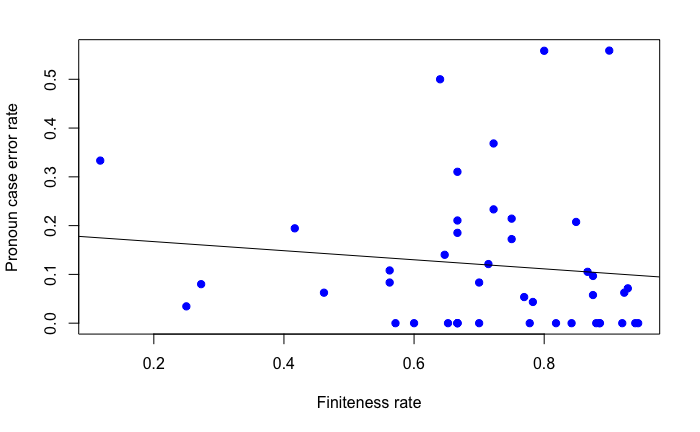
\includegraphics[scale = 0.5]{graph/Rispo1.png}
    \vspace{-1.5em}
    \caption{Pronoun case error rate by finiteness rate in CHILDES data }
    \label{fig:780}
\end{figure}
\FloatBarrier

\FloatBarrier
\begin{figure}[!h]
    \centering
    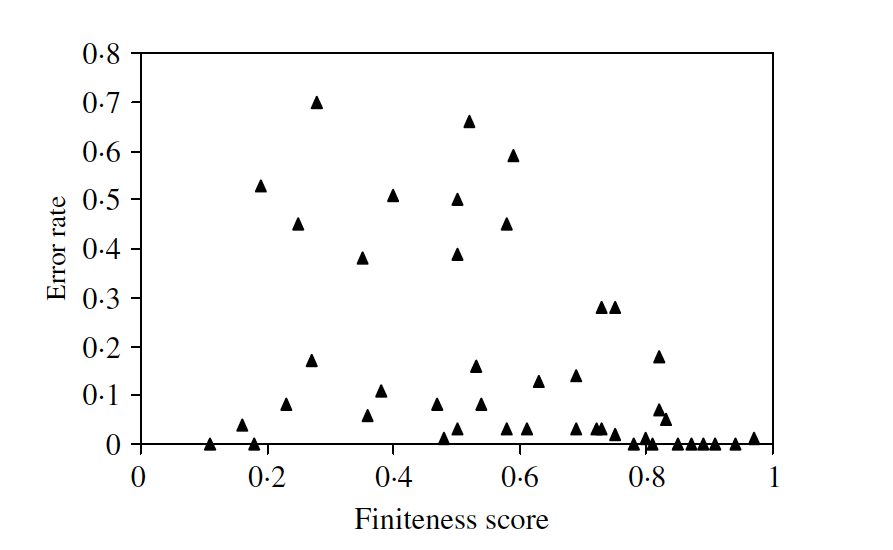
\includegraphics[scale = 0.4]{graph/Rispo2.png}
    \vspace{-1em}
    \caption{Pronoun case error rate by finiteness rate in \cite{rispoli2005}}
    \label{fig:781}
\end{figure}
\FloatBarrier

In conclusion, there is no significant correlation found between the pronoun case error rate and the finiteness rate in the CHILDES data. The regression analysis also demonstrates that the pronoun case error rate can not be predicted by verbal finiteness, age or mlu. \cite{rispoli2005}'s results were not replicated in CHILDES data.


\subsection{Conclusion}
This section reviewed the syntactic explanation for non-nominative subject errors, which claims that the use of the non-finite verbs leads to the non-nominative subject error in children's speech. It predicts that the presence of the finite verb will block the non-nominative subjects, therefore sentences like `*Her goes to the school' should almost never occur. Generally, it is difficult to test this prediction since non-nominative pronouns are rarely used as the subject. Therefore, it's difficult to judge if it is rare for the non-nominative subjects to precede a finite verb since the non-nominative subjects are uncommon. 

One way to test if the finite verb lowers the likelihood of the non-nominative pronoun is to compare the conditional probability of non-nominative subjects given finite verb P(Non-nominative|Finite) to the probability of non-nominative subjects P(Non-nominative). If P(Non-nominative|Finite) is smaller than P(Non-nominative), then it means that the presence of the finite verb actually prevents the use of non-nominative subjects. The meta-analysis shows that in general P(Non-nominative) is significantly larger than P(Non-nominative|Finite). However, depending on the child and the pronoun, P(Non-nominative) is often no different from P(Non-nominative|Finite). This result indicates that the finite verb doesn't guarantee that the subject pronoun will always get the nominative case, which is against the prediction of the syntactic explanation. In addition, the pronoun case error rate and the finiteness rate is not correlated, indicating that when children use more finite verbs, they don't necessarily make fewer pronoun case errors. The regression analysis also showed that the pronoun case error can not be predicted by finiteness rate. 

In conclusion, there is not enough evidence to support hypothesis that pronoun case errors stem from children's use of non-finite verbs. The finite verb does not always block the use of non-nominative subjects, and there is also no correlation between the finiteness rate and the pronoun case error rate. 
\newpage
%\section{Study 3. Can Parents' Input Explain Pronoun Case Errors?}

\subsection{'Let me do' it}
\newpage
%\section{Study 4. Do Children Have a Pronoun Paradigm?}

\newpage
\bibliography{bib}
\bibliographystyle{apalike}
\newpage

%\appendix
%\section{Appendix}
\begin{table}[]
\small
\centering
\caption{North American Corpus} 
%\begin{adjustbox}
\begin{tabular}{c|c|c|c|c|c}
\toprule
\textbf{Corpora}  & \textbf{Child}  & \textbf{Age} &
\textbf{Corpora}  & \textbf{Child}  & \textbf{Age}\\
\hline
\cite{bloom1974imitation}  & Peter   & 1;9-3;2 & \cite{suppes1974semantics} &  Nina & 2;0-3;4
\\
\cite{braunwald1971mother}  & Laura   & 1;5-4;0 & \cite{kuczaj1978children} &  Abe & 2;5-4;0 \\
\multirow{}{}{\cite{brown1973first}} & Adam & 2;3-4;0 & \cite{demetras1986working} & Trevor & 2;1-4;0\\
& Eve & 1;6-2;3 & \multirow{}{}{\cite{Weist2009}} & Ben & 2;4-3;4 \\
& Sarah & 2;3-4;0 & &Emily & 2;6-3;4\\
\cite{demetras1989changes} & Jimmy & 2;2-2;10 & & Emma & 2;7-3;9\\
\cite{clark1978awareness} & Shem & 2;3-3;2 &  & Jilian & 2;1-2;10\\
\cite{sachs1983talking}& Naomi & 1;3-4;9 & & Matt & 2;5-5;0\\
\cite{macwhinney2014childes} & Ross & 1;4-5;0 & & Roman & 2;3-4;0\\
\multirow{}{}{\cite{post1993language}}& She & 1;8-2;5 & \cite{Snow1990child} & Nathaniel & 3;1-3;3\\
&Tow&1;9-2;5&\cite{hayes1988vocabulary}&Geraldine&1;6-2;2\\
\hline
\hline
& \textbf{No.} & \textbf{Mean Age} & & \textbf{No.} & \textbf{Mean Age}\\
\cite{bates1991first}  & 11  & 2;4 &
\cite{bohannon1977children}  & 2 & 3;6\\
\cite{gleason1980acquisition}&19&4;8&\cite{snow1995shell}&79&3;11\\
\cite{snow1989imitativeness}&25&2;8&\cite{valian1991syntactic}&17&2;5\\
\cite{van1980effects}&19&3;9\\
\bottomrule
\end{tabular}
%\end{adjustbox}
\end{table}
\begin{table}[!]
\small
\centering
\caption{UK Corpus} 
%\begin{adjustbox}
\begin{tabular}{c|c|c|c|c|c}
\toprule
\textbf{Corpora}  & \textbf{Child}  & \textbf{Age} &
\textbf{Corpora}  & \textbf{Child}  & \textbf{Age}\\
\hline
\multirow{}{}{\cite{henry1995belfast}} & Barbara & 2;4-4;1 & \multirow{}{}{\cite{theakston2001}} & Anne & 1;10-2;9\\
& Michelle & 2;4-4;4 & & Warren& 1;10-2;9 \\
& Courtney & 3;4-4;0 & &Aran & 1;11-2;10\\
 & Rachel & 2;5-3;2 & & Becky & 2;0-2;11\\
 & Conor & 3;8-4;5 &  & Carl & 1;8-2;8\\
& Stuart & 3;5-4;5 & & Dominic & 1;10-2;10\\
 & Johnny & 3;5-4;4 & & Gail & 1;11-2;11\\
 & David & 2;0-4;2 &  & Joel & 1;11-2;10\\
\cite{rowland2006effect} & Lara & 1;9-3;3&  & John &1;11-2;10 \\
\cite{maslen2004dense} & Thomas & 2;0-4;11 & & Liz& 1;11-2;10\\
\multirow{}{}{\cite{lieven2009two}} &Eleanor &2;0-3;1 & & Nicole& 2;0-3;0 \\
&Fraser &2;0-3;0 & & Ruth& 1;11-2;11 \\
\hline
\hline
&\textbf{No.}&\textbf{Mean Age}& &\textbf{No.}&\textbf{Mean Age}\\
\cite{tommerdahl2013analyzing}&23&2;9&\cite{howe1981acquiring}&16&2;0\\
\bottomrule
\end{tabular}
%\end{adjustbox}
\end{table}


\begin{table}[]
\small
\begin{tabular}{llllllll}
name & age range & mlu range &  words & input  & pronouns & input pronouns & errors \\
\toprule
Peter & NAN & MAN & NAN & NAN & 7877 & 2384 & 155 \\
Laura & 1;5 - 7;0 & 1.0 – 6.62 & 70071 & 91822 & 10115 & 12488 & 213 \\
Adam & 2;3 - 5;2 & 2.40 – 6.46 & 175835 & 92439 & 24075 & 13235 & 589 \\
Eve & 1;6 - 2;3 & 2.09 – 4.95 & 34611 & 42601 & 4283 & 6061 & 98 \\
Sarah & 2;3 - 5;1 & 1.59 – 7.77 & 108047 & 124115 & 15472 & 16361 & 361 \\
Jimmy & 2;2 - 2;10 & 3.51 – 5.91 & 23615 & 30696 & 2761 & 2027 & 85 \\
Shem & 2;3 - 3;2 & 4.32 – 12.23 & 83536 & 10535 & 9217 & 1337 & 102 \\
Naomi & 1;3 - 4;9 & 1.30 – 7.92 & 44111 & 36079 & 5243 & 4428 & 119 \\
Ross & 0;1 - 7;8 & 1.71 - 21.0 & 165856 & 32325 & 24740 & 4944 & 397 \\
She & 1;8 - 2;5 & 2.23 - 3.55 & 6768 & 17922 & 761 & 2365 & 34 \\
Tow & 1;7 - 2;5 & 1.87 – 5.07 & 7686 & 30966 & 979 & 3871 & 64 \\
Nina & 2;0 - 3;4 & 2.25 - 6.07 & 101191 & 179999 & 11868 & 25710 & 1067 \\
Abe & 2;5 - 5;0 & 3.68 - 10.54 & 160930 & 52828 & 24820 & 8055 & 340 \\
Trevor & 2;1 - 4;0 & 4.26 – 8.04 & 26260 & 35618 & 2893 & 0 & 76 \\
Ben & 2;4 - 3;4 & 4.95 - 6.90 & 13730 & 9204 & 1638 & 1177 & 79 \\
Emily & 2;6 - 4;6 & 4.64 – 9.38 & 32325 & 1017 & 5109 & 143 & 111 \\
Emma & 2;7 - 4;8 & 3.69 – 6.40 & 26829 & 4865 & 3473 & 697 & 70 \\
Jillian & 2;1 - 2;10 & 2.77 - 7.08 & 20492 & 20226 & 2675 & 2756 & 123 \\
Matt & 2;3 - 5;0 & 2.85 - 11.09 & 46086 & 135852 & 6620 & 19669 & 101 \\
Roman & 2;3 - 4;8 & 2.98 - 11.97 & 50432 & 8848 & 6088 & 1147 & 110 \\
Nathaniel & 2;6 - 3;9 & 1.84 – 6.59 & 66036 & 121136 & 2197 & 8974 & NAN \\
Geraldine & 1;6 - 2;5 & 1.35 - 5.48 & 4564 & 16153 & 602 & 1935 & NAN \\
Anne & 1;10 - 2;9 & 1.75 - 4.15 & 50091 & 140284 & 5034 & 18766 & NAN \\
Aran & 1;11 - 2;11 & 1.46 - 5.02 & 48164 & 187083 & 7025 & 27203 & 28 \\
Barbara & 2;4 - 4;2 & 3.37 - 6.47 & 10153 & 31814 & 1354 & 5055 & 3 \\
Becky & 2;0 - 2;11 & 1.53 - 3.97 & 60488 & 97579 & 7149 & 14603 & 57 \\
Carl & 1;9 - 2;8 & 2.22 - 4.36 & 67072 & 85844 & 5513 & 10382 & 37 \\
Conor & 3;8 - 4;6 & 1.87 - 5.71 & 14832 & 52355 & 2005 & 8063 & 18 \\
Courtney & 3;4 - 4;0 & 5.13 - 6.68 & 10228 & 12036 & 1403 & 1713 & 12 \\
David & 2;0 - 4;2 & 2.32 - 6.41 & 7890 & 19966 & 1021 & 3223 & 1 \\
Dominic & 1;11 - 2;11 & 1.34 - 4.08 & 49987 & 129557 & 4969 & 18603 & 134 \\
Eleanor & 2;0 - 3;1 & 2.12 - 4.26 & 221678 & 361497 & 29191 & 48309 & 167 \\
Gail & 2;0 - 2;11 & 1.87 - 4.33 & 42233 & 104419 & 4764 & 16074 & 96 \\
Joel & 1;11 - 2;10 & 1.41 - 3.92 & 45679 & 109337 & 4984 & 15246 & 35 \\
John & 1;11 - 2;11 & 1.92 - 3.78 & 30502 & 80120 & 2181 & 10299 & 15 \\
Johnny & 3;6 - 4;4 & 3.93 - 4.52 & 6540 & 3528 & 877 & 508 & 7 \\
Lara & 1;9 - 3;4 & 1.85 - 8.0 & 175782 & 291534 & 25442 & 41210 & 188 \\
Liz & 1;11 - 2;11 & 1.52 - 4.79 & 40780 & 77560 & 5192 & 10762 & 51 \\
Michelle & 2;5 - 4;5 & 3.0 - 6.87 & 14794 & 24786 & 2401 & 3741 & 25 \\
Nicole & 2;1 - 3;0 & 1.26 - 3.61 & 36425 & 120479 & 2365 & 17915 & 38 \\
Rachel & 2;6 - 3;2 & 2.8 - 6.33 & 5932 & 20352 & 665 & 2759 & 19 \\
Ruth & 1;11 - 3;0 & 1.63 - 4.34 & 42724 & 138906 & 4129 & 19743 & 75 \\
Stuart & 3;5 - 4;5 & 4.51 - 6.34 & 16678 & 16085 & 2372 & 2403 & 27 \\
Thomas & 2;0 - 5;0 & 1.56 - 6.92 & 554257 & 1823256 & 48563 & 227178 & 410 \\
Warren & 1;10 - 2;10 & 2.02 - 4.71 & 49155 & 118113 & 4071 & 14859 & 116
\end{tabular}
\end{table}
%%%Anne
\begin{table}[]
    \caption{Anne ATOM Model}
\begin{minipage}{0.5\textwidth}
    \centering
    \subcaption{1sg Finiteness Versus Case}
    \begin{tabular}{@{}lll@{}}
        \toprule
         &\multicolumn{2}{c}{Verb form}\\
         \cline{2-3}
        Subject & Finite & -Finite \\
        \midrule
        I & 346 & 45 \\
        me + my & 5 & 78 \\
        \hline
        \%non-NOM & 1\% & 63\% \\
        \bottomrule
    \end{tabular}
\end{minipage}
\begin{minipage}{0.5\textwidth}
    \centering
    \subcaption{3sg Finiteness Versus Case}
    \begin{tabular}{@{}lll@{}}
        \toprule
         &\multicolumn{2}{c}{Verb form}\\
         \cline{2-3}
        Subject & Finite & -Finite \\
        \midrule
        he + she & 133 & 78 \\
        him + her & 8 & 36 \\
        \hline
        \%non-NOM & 6\% & 32\% \\
        \bottomrule
    \end{tabular}
    \end{minipage}
\begin{minipage}{0.5\textwidth}
    \subcaption{1sg Distribution by Verb type}
        \centering
    \begin{tabular}{@{}llll@{}}
        \toprule
            &\multicolumn{3}{c}{Subject Form}\\
            \cline{2-4}
        Verb Form & I & me & my \\
        \midrule
        Auxiliary & 25 & 0 & 0 \\
        Modal & 188 & 1 & 1 \\
        Copula & 14 & 1 & 0 \\
        Past Tense & 119 & 2 & 0 \\
        \hline
        Null Auxiliary & 31 & 6 & 13 \\
        Null Copula & 14 & 39 & 20 \\
        \bottomrule
    \end{tabular}
\end{minipage}
\begin{minipage}{0.5\textwidth}
    \subcaption{3sg pronoun}
        \centering
    \begin{tabular}{@{}lllll@{}}
        \toprule
            &\multicolumn{4}{c}{Subject Form}\\
            \cline{2-5}
        Verb form & he & him & she & her \\
        \midrule
        Main V with -s & 27 & 0 & 1 & 3 \\
        Aux with -s & 7 & 0 & 0 & 0 \\
        Modal & 29 & 1 & 5 & 0 \\
        Copula with -s & 19 & 0 & 0 & 1 \\
        Past Tense & 33 & 1 & 12 & 2 \\
        \hline
        Main V without -s & 22 & 3 & 4 & 3 \\
        Aux with -s & 2 & 0 & 1 & 0 \\
        Null Auxiliary & 28 & 0 & 6 & 3 \\
        Null Copula & 6 & 23 & 9 & 4 \\
        \bottomrule
    \end{tabular}
    \end{minipage}
\end{table}
%%%Aran
\begin{table}[]
    \caption{Aran ATOM Model}
\begin{minipage}{0.5\textwidth}
    \centering
    \subcaption{1sg Finiteness Versus Case}
    \begin{tabular}{@{}lll@{}}
        \toprule
         &\multicolumn{2}{c}{Verb form}\\
         \cline{2-3}
        Subject & Finite & -Finite \\
        \midrule
        I & 774 & 69 \\
        me + my & 5 & 72 \\
        \hline
        \%non-NOM & 1\% & 51\% \\
        \bottomrule
    \end{tabular}
\end{minipage}
\begin{minipage}{0.5\textwidth}
    \centering
    \subcaption{3sg Finiteness Versus Case}
    \begin{tabular}{@{}lll@{}}
        \toprule
         &\multicolumn{2}{c}{Verb form}\\
         \cline{2-3}
        Subject & Finite & -Finite \\
        \midrule
        he + she & 197 & 102 \\
        him + her & 0 & 43 \\
        \hline
        \%non-NOM & 0\% & 30\% \\
        \bottomrule
    \end{tabular}
    \end{minipage}
    \begin{minipage}{0.5\textwidth}
    \centering
    \subcaption{1sg Distribution by Verb type}
    \begin{tabular}{@{}llll@{}}
        \toprule
            &\multicolumn{3}{l}{Subject Form}\\
            \cline{2-4}
        Verb Form & I & me & my \\
        \midrule
        Auxiliary & 26 & 0 & 0 \\
        Modal & 467 & 1 & 0 \\
        Copula & 25 & 0 & 0 \\
        Past Tense & 256 & 4 & 0 \\
        \hline
        Null Auxiliary & 28 & 5 & 5 \\
        Null Copula & 41 & 40 & 22 \\
        \bottomrule
    \end{tabular}
\end{minipage}
\begin{minipage}{0.5\textwidth}
    \centering
    \subcaption{3sg Distribution by Verb type}
    \begin{tabular}{@{}lllll@{}}
        \toprule
            &\multicolumn{4}{l}{Subject Form}\\
            \cline{2-5}
        Verb form & he & him & she & her \\
        \midrule
        Main V with -s & 31 & 0 & 0 & 0 \\
        Aux with -s & 3 & 0 & 0 & 0 \\
        Modal & 79 & 0 & 0 & 0 \\
        Copula with -s & 9 & 0 & 0 & 0 \\
        Past Tense & 70 & 0 & 5 & 0 \\
        \hline
        Main V without -s & 59 & 1 & 2 & 1 \\
        Aux with -s & 3 & 0 & 0 & 0 \\
        Null Auxiliary & 19 & 1 & 0 & 3 \\
        Null Copula & 19 & 33 & 0 & 4 \\
        \bottomrule
    \end{tabular}
    \end{minipage}
\end{table}
%%%Barbara
\begin{table}[]
    \caption{Barbara ATOM Model}
\begin{minipage}{0.5\textwidth}
    \centering
    \subcaption{1sg Finiteness Versus Case}
    \begin{tabular}{@{}lll@{}}
        \toprule
         &\multicolumn{2}{c}{Verb form}\\
         \cline{2-3}
        Subject & Finite & -Finite \\
        \midrule
        I & 198 & 15 \\
        me + my & 2 & 21 \\
        \hline
        \%non-NOM & 1\% & 58\% \\
        \bottomrule
    \end{tabular}
\end{minipage}
\begin{minipage}{0.5\textwidth}
    \centering
    \subcaption{3sg Finiteness Versus Case}
    \begin{tabular}{@{}lll@{}}
        \toprule
         &\multicolumn{2}{c}{Verb form}\\
         \cline{2-3}
        Subject & Finite & -Finite \\
        \midrule
        he + she & 142 & 52 \\
        him + her & 0 & 6 \\
        \hline
        \%non-NOM & 0\% & 10\% \\
        \bottomrule
    \end{tabular}
    \end{minipage}
    \begin{minipage}{0.5\textwidth}
    \centering
    \subcaption{1sg Distribution by Verb type}
    \begin{tabular}{@{}llll@{}}
        \toprule
            &\multicolumn{3}{l}{Subject Form}\\
            \cline{2-4}
        Verb form & I & me & my \\
        \midrule
        Auxiliary & 11 & 0 & 0 \\
        Modal & 100 & 2 & 0 \\
        Copula & 5 & 0 & 0 \\
        Past Tense & 82 & 0 & 0 \\
        \hline
        Null Auxiliary & 7 & 2 & 0 \\
        Null Copula & 8 & 1 & 18 \\
        \bottomrule
    \end{tabular}
\end{minipage}
\begin{minipage}{0.5\textwidth}
\centering
    \subcaption{3sg Distribution by Verb type}
    \begin{tabular}{@{}lllll@{}}
        \toprule
            &\multicolumn{4}{l}{Subject Form}\\
            \cline{2-5}
        Verb form & he & him & she & her \\
        \midrule
        Main V with -s & 12 & 0 & 18 & 0 \\
        Aux with -s & 0 & 0 & 2 & 0 \\
        Modal & 11 & 0 & 21 & 0 \\
        Copula with -s & 5 & 0 & 1 & 0 \\
        Past Tense & 32 & 0 & 40 & 0 \\
        \hline
        Main V without -s & 14 & 1 & 6 & 1 \\
        Aux with -s & 0 & 0 & 0 & 0 \\
        Null Auxiliary & 13 & 0 & 13 & 0 \\
        Null Copula & 5 & 4 & 1 & 0 \\
        \bottomrule
    \end{tabular}
    \end{minipage}
\end{table}
%%%Becky
\begin{table}[]
    \caption{Becky ATOM Model}
    \begin{minipage}{0.5\textwidth}
    \centering
    \subcaption{1sg Finiteness Versus Case}
    \begin{tabular}{@{}lll@{}}
        \toprule
         &\multicolumn{2}{c}{Verb form}\\
         \cline{2-3}
        Subject & Finite & -Finite \\
        \midrule
        I & 961 & 193 \\
        me + my & 7 & 41 \\
        \hline
        \%non-NOM & 1\% & 18\% \\
        \bottomrule
    \end{tabular}
\end{minipage}
\begin{minipage}{0.5\textwidth}
    \centering
    \subcaption{3sg Finiteness Versus Case}
    \begin{tabular}{@{}lll@{}}
        \toprule
         &\multicolumn{2}{c}{Verb form}\\
         \cline{2-3}
        Subject & Finite & -Finite \\
        \midrule
        he + she & 204 & 145 \\
        him + her & 13 & 42 \\
        \hline
        \%non-NOM & 6\% & 22\% \\
        \bottomrule
    \end{tabular}
    \end{minipage}
    \begin{minipage}{0.5\textwidth}
    \centering
    \subcaption{1sg Distribution by Verb type}
    \begin{tabular}{@{}llll@{}}
        \toprule
            &\multicolumn{3}{l}{Subject Form}\\
            \cline{2-4}
        Verb form & I & me & my \\
        \midrule
        Auxiliary & 50 & 0 & 0 \\
        Modal & 438 & 2 & 1 \\
        Copula & 41 & 2 & 0 \\
        Past Tense & 432 & 1 & 1 \\
        \hline
        Null Auxiliary & 130 & 2 & 6 \\
        Null Copula & 63 & 21 & 12 \\
        \bottomrule
    \end{tabular}
\end{minipage}
\begin{minipage}{0.5\textwidth}
    \centering
    \subcaption{3sg Distribution by Verb type}
    \begin{tabular}{@{}lllll@{}}
        \toprule
            &\multicolumn{4}{l}{Subject Form}\\
            \cline{2-5}
        Verb form & he & him & she & her \\
        \midrule
        Main V with -s & 25 & 0 & 11 & 0 \\
        Aux with -s & 11 & 0 & 0 & 5 \\
        Modal & 51 & 1 & 18 & 0 \\
        Copula with -s & 19 & 0 & 4 & 1 \\
        Past Tense & 50 & 2 & 15 & 4 \\
        \hline
        Main V without -s & 56 & 6 & 15 & 1 \\
        Aux with -s & 4 & 0 & 2 & 0 \\
        Null Auxiliary & 45 & 1 & 4 & 3 \\
        Null Copula & 16 & 28 & 3 & 3 \\
        \bottomrule
    \end{tabular}
    \end{minipage}
\end{table}
%%%Carl
\begin{table}[]
    \caption{Carl's ATOM Model}
    \begin{minipage}{0.5\textwidth}
    \centering
    \subcaption{1sg Finiteness Versus Case}
    \begin{tabular}{@{}lll@{}}
        \toprule
         &\multicolumn{2}{c}{Verb form}\\
         \cline{2-3}
        Subject & Finite & -Finite \\
        \midrule
        I & 611 & 273 \\
        me + my & 5 & 26 \\
        \hline
        \%non-NOM & 1\% & 9\% \\
        \bottomrule
    \end{tabular}
\end{minipage}
\begin{minipage}{0.5\textwidth}
    \centering
    \subcaption{3sg Finiteness Versus Case}
    \begin{tabular}{@{}lll@{}}
        \toprule
         &\multicolumn{2}{c}{Verb form}\\
         \cline{2-3}
        Subject & Finite & -Finite \\
        \midrule
        he + she & 324 & 371 \\
        him + her & 0 & 9 \\
        \hline
        \%non-NOM & 0\% & 2\% \\
        \bottomrule
    \end{tabular}
    \end{minipage}
    \begin{minipage}{0.5\textwidth}
    \centering
    \subcaption{1sg Distribution by Verb type}
    \begin{tabular}{@{}llll@{}}
        \toprule
            &\multicolumn{3}{l}{Subject Form}\\
            \cline{2-4}
        Verb form & I & me & my \\
        \midrule
        Auxiliary & 2 & 0 & 0 \\
        Modal & 351 & 0 & 0 \\
        Copula & 6 & 0 & 0 \\
        Past Tense & 252 & 3 & 2 \\
        \hline
        Null Auxiliary & 232 & 2 & 6 \\
        Null Copula & 41 & 5 & 13 \\
        \bottomrule
    \end{tabular}
\end{minipage}
\begin{minipage}{0.5\textwidth}
    \centering
    \subcaption{3sg Distribution by Verb type}
    \begin{tabular}{@{}lllll@{}}
        \toprule
            &\multicolumn{4}{l}{Subject Form}\\
            \cline{2-5}
        Verb form & he & him & she & her \\
        \midrule
        Main V with -s & 67 & 0 & 0 & 0 \\
        Aux with -s & 0 & 0 & 0 & 0 \\
        Modal & 89 & 0 & 0 & 0 \\
        Copula with -s & 9 & 0 & 0 & 0 \\
        Past Tense & 156 & 0 & 3 & 0 \\
        \hline
        Main V without -s & 228 & 0 & 4 & 0 \\
        Aux with -s & 0 & 0 & 0 & 0 \\
        Null Auxiliary & 98 & 0 & 1 & 0 \\
        Null Copula & 39 & 9 & 1 & 0 \\
        \bottomrule
    \end{tabular}
    \end{minipage}
\end{table}
%%%Conor
\begin{table}[]
    \caption{Conor ATOM Model}
    \begin{minipage}{0.5\textwidth}
    \centering
    \subcaption{1sg Finiteness Versus Case}
    \begin{tabular}{@{}lll@{}}
        \toprule
         &\multicolumn{2}{c}{Verb form}\\
         \cline{2-3}
        Subject & Finite & -Finite \\
        \midrule
        I & 215 & 27 \\
        me + my & 0 & 25 \\
        \hline
        \%non-NOM & 0\% & 48\% \\
        \bottomrule
    \end{tabular}
\end{minipage}
\begin{minipage}{0.5\textwidth}
    \centering
    \subcaption{3sg Finiteness Versus Case}
    \begin{tabular}{@{}lll@{}}
        \toprule
         &\multicolumn{2}{c}{Verb form}\\
         \cline{2-3}
        Subject & Finite & -Finite \\
        \midrule
        he + she & 210 & 34 \\
        him + her & 0 & 27 \\
        \hline
        \%non-NOM & 0\% & 44\% \\
        \bottomrule
    \end{tabular}
    \end{minipage}
    \begin{minipage}{0.5\textwidth}
    \centering
    \subcaption{1sg Distribution by Verb type}
    \begin{tabular}{@{}llll@{}}
        \toprule
            &\multicolumn{3}{l}{Subject Form}\\
            \cline{2-4}
        Verb form & I & me & my \\
        \midrule
        Auxiliary & 14 & 0 & 0 \\
        Modal & 92 & 0 & 0 \\
        Copula & 13 & 0 & 0 \\
        Past Tense & 96 & 0 & 0 \\
        \hline
        Null Auxiliary & 13 & 5 & 0 \\
        Null Copula & 14 & 7 & 13 \\
        \bottomrule
    \end{tabular}
\end{minipage}
\begin{minipage}{0.5\textwidth}
    \centering
    \subcaption{3sg Distribution by Verb type}
    \begin{tabular}{@{}lllll@{}}
        \toprule
            &\multicolumn{4}{l}{Subject Form}\\
            \cline{2-5}
        Verb form & he & him & she & her \\
        \midrule
        Main V with -s & 62 & 0 & 7 & 0 \\
        Aux with -s & 7 & 0 & 7 & 0 \\
        Modal & 26 & 0 & 10 & 0 \\
        Copula with -s & 19 & 0 & 2 & 0 \\
        Past Tense & 50 & 0 & 20 & 0 \\
        \hline
        Main V without -s & 10 & 2 & 3 & 0 \\
        Aux with -s & 0 & 0 & 0 & 0 \\
        Null Auxiliary & 9 & 0 & 4 & 1 \\
        Null Copula & 7 & 24 & 1 & 0 \\
        \bottomrule
    \end{tabular}
    \end{minipage}
\end{table}
%%%Courtney
\begin{table}[]
    \caption{Courtney ATOM Model}
    \begin{minipage}{0.5\textwidth}
    \centering
    \subcaption{1sg Finiteness Versus Case}
    \begin{tabular}{@{}lll@{}}
        \toprule
         &\multicolumn{2}{c}{Verb form}\\
         \cline{2-3}
        Subject & Finite & -Finite \\
        \midrule
        I & 211 & 6 \\
        me + my & 0 & 20 \\
        \hline
        \%non-NOM & 0\% & 77\% \\
        \bottomrule
    \end{tabular}
\end{minipage}
\begin{minipage}{0.5\textwidth}
    \centering
    \subcaption{3sg Finiteness Versus Case}
    \begin{tabular}{@{}lll@{}}
        \toprule
         &\multicolumn{2}{c}{Verb form}\\
         \cline{2-3}
        Subject & Finite & -Finite \\
        \midrule
        he + she & 137 & 17 \\
        him + her & 3 & 25 \\
        \hline
        \%non-NOM & 2\% & 60\% \\
        \bottomrule
    \end{tabular}
    \end{minipage}
    \begin{minipage}{0.5\textwidth}
    
    \centering
    \subcaption{1sg Distribution by Verb type}
    \begin{tabular}{@{}llll@{}}
        \toprule
            &\multicolumn{3}{l}{Subject Form}\\
            \cline{2-4}
        Verb form & I & me & my \\
        \midrule
        Auxiliary & 11 & 0 & 0 \\
        Modal & 109 & 0 & 0 \\
        Copula & 2 & 0 & 0 \\
        Past Tense & 89 & 0 & 0 \\
        \hline
        Null Auxiliary & 5 & 1 & 0 \\
        Null Copula & 1 & 10 & 9 \\
        \bottomrule
    \end{tabular}
\end{minipage}
\begin{minipage}{0.5\textwidth}
    \centering
    \subcaption{3sg Distribution by Verb type}
    \begin{tabular}{@{}lllll@{}}
        \toprule
            &\multicolumn{4}{l}{Subject Form}\\
            \cline{2-5}
        Verb form & he & him & she & her \\
        \midrule
        Main V with -s & 28 & 0 & 9 & 0 \\
        Aux with -s & 0 & 0 & 4 & 0 \\
        Modal & 39 & 1 & 14 & 1 \\
        Copula with -s & 3 & 0 & 2 & 0 \\
        Past Tense & 24 & 0 & 14 & 1 \\
        \hline
        Main V without -s & 7 & 6 & 2 & 0 \\
        Aux with -s & 0 & 0 & 0 & 2 \\
        Null Auxiliary & 1 & 1 & 1 & 2 \\
        Null Copula & 3 & 13 & 3 & 1 \\
        \bottomrule
    \end{tabular}
    \end{minipage}
\end{table}
%%%David
\begin{table}[]
    \caption{David ATOM Model}
    \begin{minipage}{0.5\textwidth}
    \centering
    \subcaption{1sg Finiteness Versus Case}
    \begin{tabular}{@{}lll@{}}
        \toprule
         &\multicolumn{2}{c}{Verb form}\\
         \cline{2-3}
        Subject & Finite & -Finite \\
        \midrule
        I & 212 & 24 \\
        me + my & 1 & 8 \\
        \hline
        \%non-NOM & 0\% & 25\% \\
        \bottomrule
    \end{tabular}
\end{minipage}
\begin{minipage}{0.5\textwidth}
    \centering
    \subcaption{3sg Finiteness Versus Case}
    \begin{tabular}{@{}lll@{}}
        \toprule
         &\multicolumn{2}{c}{Verb form}\\
         \cline{2-3}
        Subject & Finite & -Finite \\
        \midrule
        he + she & 50 & 31 \\
        him + her & 0 & 1 \\
        \hline
        \%non-NOM & 0\% & 3\% \\
        \bottomrule
    \end{tabular}
    \end{minipage}
    \begin{minipage}{0.5\textwidth}
    
    \centering
    \subcaption{1sg Distribution by Verb type}
    \begin{tabular}{@{}llll@{}}
        \toprule
            &\multicolumn{3}{l}{Subject Form}\\
            \cline{2-4}
        Verb form & I & me & my \\
        \midrule
        Auxiliary & 8 & 0 & 0 \\
        Modal & 114 & 0 & 0 \\
        Copula & 9 & 0 & 0 \\
        Past Tense & 81 & 1 & 0 \\
        \hline
        Null Auxiliary & 17 & 2 & 2 \\
        Null Copula & 7 & 0 & 4 \\
        \bottomrule
    \end{tabular}
\end{minipage}
\begin{minipage}{0.5\textwidth}
    \centering
    \subcaption{3sg Distribution by Verb type}
    \begin{tabular}{@{}lllll@{}}
        \toprule
            &\multicolumn{4}{l}{Subject Form}\\
            \cline{2-5}
        Verb form & he & him & she & her \\
        \midrule
        Main V with -s & 8 & 0 & 1 & 0 \\
        Aux with -s & 0 & 0 & 0 & 0 \\
        Modal & 5 & 0 & 1 & 0 \\
        Copula with -s & 0 & 0 & 0 & 0 \\
        Past Tense & 22 & 0 & 13 & 0 \\
        \hline
        Main V without -s & 17 & 0 & 3 & 0 \\
        Aux with -s & 0 & 0 & 0 & 0 \\
        Null Auxiliary & 5 & 0 & 3 & 0 \\
        Null Copula & 2 & 1 & 1 & 0 \\
        \bottomrule
    \end{tabular}
    \end{minipage}
\end{table}

%%%Dominic
\begin{table}[]
    \caption{Dominic ATOM Model}
    \begin{minipage}{0.5\textwidth}
    \centering
    \subcaption{1sg Finiteness Versus Case}
    \begin{tabular}{@{}lll@{}}
        \toprule
         &\multicolumn{2}{c}{Verb form}\\
         \cline{2-3}
        Subject & Finite & -Finite \\
        \midrule
        I & 620 & 150 \\
        me + my & 5 & 31 \\
        \hline
        \%non-NOM & 1\% & 17\% \\
        \bottomrule
    \end{tabular}
\end{minipage}
\begin{minipage}{0.5\textwidth}
    \centering
    \subcaption{3sg Finiteness Versus Case}
    \begin{tabular}{@{}lll@{}}
        \toprule
         &\multicolumn{2}{c}{Verb form}\\
         \cline{2-3}
        Subject & Finite & -Finite \\
        \midrule
        he + she & 53 & 39 \\
        him + her & 1 & 1 \\
        \hline
        \%non-NOM & 2\% & 2\% \\
        \bottomrule
    \end{tabular}
    \end{minipage}
    \begin{minipage}{0.5\textwidth}
    \centering
    \subcaption{1sg Distribution by Verb type}
    \begin{tabular}{@{}llll@{}}
        \toprule
            &\multicolumn{3}{l}{Subject Form}\\
            \cline{2-4}
        Verb form & I & me & my \\
        \midrule
        Auxiliary & 30 & 0 & 0 \\
        Modal & 318 & 0 & 1 \\
        Copula & 44 & 0 & 0 \\
        Past Tense & 228 & 2 & 2 \\
        \hline
        Null Auxiliary & 128 & 1 & 6 \\
        Null Copula & 22 & 3 & 21 \\
        \bottomrule
    \end{tabular}
\end{minipage}
\begin{minipage}{0.5\textwidth}
    \centering
    \subcaption{3sg Distribution by Verb type}
    \begin{tabular}{@{}lllll@{}}
        \toprule
            &\multicolumn{4}{l}{Subject Form}\\
            \cline{2-5}
        Verb form & he & him & she & her \\
        \midrule
        Main V with -s & 12 & 0 & 2 & 1 \\
        Aux with -s & 5 & 0 & 0 & 0 \\
        Modal & 9 & 0 & 1 & 0 \\
        Copula with -s & 4 & 0 & 0 & 0 \\
        Past Tense & 16 & 0 & 4 & 0 \\
        \hline
        Main V without -s & 11 & 0 & 1 & 0 \\
        Aux with -s & 0 & 0 & 0 & 0 \\
        Null Auxiliary & 13 & 0 & 2 & 0 \\
        Null Copula & 11 & 1 & 1 & 0 \\
        \bottomrule
    \end{tabular}
    \end{minipage}
\end{table}
%%%Eleanor

\begin{table}[]
    \caption{Eleanor's ATOM Model}
    \begin{minipage}{0.5\textwidth}
    \centering
    \subcaption{1sg Finiteness Versus Case}
    \begin{tabular}{@{}lll@{}}
        \toprule
         &\multicolumn{2}{c}{Verb form}\\
         \cline{2-3}
        Subject & Finite & -Finite \\
        \midrule
        I & 4069 & 689 \\
        me + my & 12 & 206 \\
        \hline
        \%non-NOM & 0\% & 23\% \\
        \bottomrule
    \end{tabular}
\end{minipage}
\begin{minipage}{0.5\textwidth}
    \centering
    \subcaption{3sg Finiteness Versus Case}
    \begin{tabular}{@{}lll@{}}
        \toprule
         &\multicolumn{2}{c}{Verb form}\\
         \cline{2-3}
        Subject & Finite & -Finite \\
        \midrule
        he + she & 822 & 251 \\
        him + her & 0 & 100 \\
        \hline
        \%non-NOM & 0\% & 28\% \\
        \bottomrule
    \end{tabular}
    \end{minipage}
    \begin{minipage}{0.5\textwidth}
    
    \centering
    \subcaption{1sg Distribution by Verb type}
    \begin{tabular}{@{}llll@{}}
        \toprule
            &\multicolumn{3}{l}{Subject Form}\\
            \cline{2-4}
        Verb form & I & me & my \\
        \midrule
        Auxiliary & 137 & 0 & 0 \\
        Modal & 2475 & 2 & 0 \\
        Copula & 154 & 0 & 1 \\
        Past Tense & 1303 & 5 & 4 \\
        \hline
        Null Auxiliary & 413 & 10 & 19 \\
        Null Copula & 276 & 61 & 116 \\
        \bottomrule
    \end{tabular}
\end{minipage}
\begin{minipage}{0.5\textwidth}
    \centering
    \subcaption{3sg Distribution by Verb type}
    \begin{tabular}{@{}lllll@{}}
        \toprule
            &\multicolumn{4}{l}{Subject Form}\\
            \cline{2-5}
        Verb form & he & him & she & her \\
        \midrule
        Main V with -s & 109 & 0 & 65 & 0 \\
        Aux with -s & 20 & 0 & 12 & 0 \\
        Modal & 144 & 0 & 80 & 0 \\
        Copula with -s & 82 & 0 & 33 & 0 \\
        Past Tense & 190 & 0 & 87 & 0 \\
        \hline
        Main V without -s & 89 & 4 & 37 & 2 \\
        Aux with -s & 5 & 0 & 3 & 0 \\
        Null Auxiliary & 51 & 2 & 25 & 0 \\
        Null Copula & 30 & 80 & 11 & 12 \\
        \bottomrule
    \end{tabular}
    \end{minipage}
\end{table}
%%%Gail

\begin{table}[]
    \caption{Gail's ATOM Model}
    \begin{minipage}{0.5\textwidth}
    \centering
    \subcaption{1sg Finiteness Versus Case}
    \begin{tabular}{@{}lll@{}}
        \toprule
         &\multicolumn{2}{c}{Verb form}\\
         \cline{2-3}
        Subject & Finite & -Finite \\
        \midrule
        I & 456 & 159 \\
        me + my & 5 & 57 \\
        \hline
        \%non-NOM & 1\% & 26\% \\
        \bottomrule
    \end{tabular}
\end{minipage}
\begin{minipage}{0.5\textwidth}
    \centering
    \subcaption{3sg Finiteness Versus Case}
    \begin{tabular}{@{}lll@{}}
        \toprule
         &\multicolumn{2}{c}{Verb form}\\
         \cline{2-3}
        Subject & Finite & -Finite \\
        \midrule
        he + she & 75 & 24 \\
        him + her & 11 & 49 \\
        \hline
        \%non-NOM & 13\% & 67\% \\
        \bottomrule
    \end{tabular}
    \end{minipage}
    \begin{minipage}{0.5\textwidth}
    \centering
    \subcaption{1sg Distribution by Verb type}
    \begin{tabular}{@{}llll@{}}
        \toprule
            &\multicolumn{3}{l}{Subject Form}\\
            \cline{2-4}
        Verb form & I & me & my \\
        \midrule
        Auxiliary & 17 & 0 & 0 \\
        Modal & 241 & 1 & 0 \\
        Copula & 13 & 0 & 0 \\
        Past Tense & 185 & 0 & 4 \\
        \hline
        Null Auxiliary & 115 & 0 & 14 \\
        Null Copula & 44 & 14 & 29 \\
        \bottomrule
    \end{tabular}
\end{minipage}
\begin{minipage}{0.5\textwidth}
    \centering
    \subcaption{3sg Distribution by Verb type}
    \begin{tabular}{@{}lllll@{}}
        \toprule
            &\multicolumn{4}{l}{Subject Form}\\
            \cline{2-5}
        Verb form & he & him & she & her \\
        \midrule
        Main V with -s & 8 & 0 & 1 & 0 \\
        Aux with -s & 4 & 0 & 0 & 0 \\
        Modal & 17 & 0 & 0 & 0 \\
        Copula with -s & 12 & 0 & 2 & 0 \\
        Past Tense & 29 & 1 & 2 & 10 \\
        \hline
        Main V without -s & 12 & 4 & 0 & 7 \\
        Aux with -s & 1 & 0 & 0 & 1 \\
        Null Auxiliary & 7 & 3 & 2 & 12 \\
        Null Copula & 2 & 18 & 0 & 4 \\
        \bottomrule
    \end{tabular}
    \end{minipage}
\end{table}
%%%Joel

\begin{table}[]
    \caption{Joel's ATOM Model}
    \begin{minipage}{0.5\textwidth}
    \centering
    \subcaption{1sg Finiteness Versus Case}
    \begin{tabular}{@{}lll@{}}
        \toprule
         &\multicolumn{2}{c}{Verb form}\\
         \cline{2-3}
        Subject & Finite & -Finite \\
        \midrule
        I & 569 & 118 \\
        me + my & 2 & 45 \\
        \hline
        \%non-NOM & 0\% & 28\% \\
        \bottomrule
    \end{tabular}
\end{minipage}
\begin{minipage}{0.5\textwidth}
    \centering
    \subcaption{3sg Finiteness Versus Case}
    \begin{tabular}{@{}lll@{}}
        \toprule
         &\multicolumn{2}{c}{Verb form}\\
         \cline{2-3}
        Subject & Finite & -Finite \\
        \midrule
        he + she & 128 & 62 \\
        him + her & 1 & 40 \\
        \hline
        \%non-NOM & 1\% & 39\% \\
        \bottomrule
    \end{tabular}
    \end{minipage}
    \begin{minipage}{0.5\textwidth}
    
    \centering
    \subcaption{1sg Distribution by Verb type}
    \begin{tabular}{@{}llll@{}}
        \toprule
            &\multicolumn{3}{l}{Subject Form}\\
            \cline{2-4}
        Verb form & I & me & my \\
        \midrule
        Auxiliary & 17 & 0 & 0 \\
        Modal & 187 & 1 & 0 \\
        Copula & 31 & 0 & 0 \\
        Past Tense & 334 & 1 & 0 \\
        \hline
        Null Auxiliary & 79 & 0 & 10 \\
        Null Copula & 39 & 16 & 19 \\
        \bottomrule
    \end{tabular}
\end{minipage}
\begin{minipage}{0.5\textwidth}
    \centering
    \subcaption{3sg Distribution by Verb type}
    \begin{tabular}{@{}lllll@{}}
        \toprule
            &\multicolumn{4}{l}{Subject Form}\\
            \cline{2-5}
        Verb form & he & him & she & her \\
        \midrule
        Main V with -s & 33 & 0 & 2 & 0 \\
        Aux with -s & 0 & 0 & 0 & 0 \\
        Modal & 21 & 1 & 2 & 0 \\
        Copula with -s & 16 & 0 & 0 & 0 \\
        Past Tense & 50 & 0 & 4 & 0 \\
        \hline
        Main V without -s & 32 & 2 & 3 & 1 \\
        Aux with -s & 1 & 2 & 0 & 0 \\
        Null Auxiliary & 17 & 0 & 5 & 0 \\
        Null Copula & 4 & 35 & 0 & 0 \\
        \bottomrule
    \end{tabular}
    \end{minipage}
\end{table}
%%%John

\begin{table}[]
    \caption{John's ATOM Model}
    \begin{minipage}{0.5\textwidth}
    \centering
    \subcaption{1sg Finiteness Versus Case}
    \begin{tabular}{@{}lll@{}}
        \toprule
         &\multicolumn{2}{c}{Verb form}\\
         \cline{2-3}
        Subject & Finite & -Finite \\
        \midrule
        I & 186 & 75 \\
        me + my & 1 & 8 \\
        \hline
        \%non-NOM & 1\% & 10\% \\
        \bottomrule
    \end{tabular}
\end{minipage}
\begin{minipage}{0.5\textwidth}
    \centering
    \subcaption{3sg Finiteness Versus Case}
    \begin{tabular}{@{}lll@{}}
        \toprule
         &\multicolumn{2}{c}{Verb form}\\
         \cline{2-3}
        Subject & Finite & -Finite \\
        \midrule
        he + she & 8 & 22 \\
        him + her & 0 & 4 \\
        \hline
        \%non-NOM & 0\% & 15\% \\
        \bottomrule
    \end{tabular}
    \end{minipage}
    \begin{minipage}{0.5\textwidth}
    
    \centering
    \subcaption{1sg Distribution by Verb type}
    \begin{tabular}{@{}llll@{}}
        \toprule
            &\multicolumn{3}{l}{Subject Form}\\
            \cline{2-4}
        Verb form & I & me & my \\
        \midrule
        Auxiliary & 1 & 0 & 0 \\
        Modal & 62 & 0 & 0 \\
        Copula & 2 & 0 & 0 \\
        Past Tense & 121 & 1 & 0 \\
        \hline
        Null Auxiliary & 55 & 0 & 0 \\
        Null Copula & 20 & 2 & 6 \\
        \bottomrule
    \end{tabular}
\end{minipage}
\begin{minipage}{0.5\textwidth}
    \centering
    \subcaption{3sg Distribution by Verb type}
    \begin{tabular}{@{}lllll@{}}
        \toprule
            &\multicolumn{4}{l}{Subject Form}\\
            \cline{2-5}
        Verb form & he & him & she & her \\
        \midrule
        Main V with -s & 1 & 0 & 0 & 0 \\
        Aux with -s & 0 & 0 & 0 & 0 \\
        Modal & 0 & 0 & 0 & 0 \\
        Copula with -s & 3 & 0 & 0 & 0 \\
        Past Tense & 2 & 0 & 2 & 0 \\
        \hline
        Main V without -s & 6 & 0 & 6 & 0 \\
        Aux with -s & 0 & 0 & 0 & 0 \\
        Null Auxiliary & 4 & 0 & 4 & 0 \\
        Null Copula & 0 & 4 & 2 & 0 \\
        \bottomrule
    \end{tabular}
    \end{minipage}
\end{table}
%%%Johnny
\begin{table}[]
    \caption{Johnny ATOM Model}
    \begin{minipage}{0.5\textwidth}
    \centering
    \subcaption{1sg Finiteness Versus Case}
    \begin{tabular}{@{}lll@{}}
        \toprule
         &\multicolumn{2}{c}{Verb form}\\
         \cline{2-3}
        Subject & Finite & -Finite \\
        \midrule
        I & 138 & 6 \\
        me + my & 0 & 16 \\
        \hline
        \%non-NOM & 0\% & 73\% \\
        \bottomrule
    \end{tabular}
\end{minipage}
\begin{minipage}{0.5\textwidth}
    \centering
    \subcaption{3sg Finiteness Versus Case}
    \begin{tabular}{@{}lll@{}}
        \toprule
         &\multicolumn{2}{c}{Verb form}\\
         \cline{2-3}
        Subject & Finite & -Finite \\
        \midrule
        he + she & 52 & 12 \\
        him + her & 0 & 4 \\
        \hline
        \%non-NOM & 0\% & 25\% \\
        \bottomrule
    \end{tabular}
    \end{minipage}
    \begin{minipage}{0.5\textwidth}
    
    \centering
    \subcaption{1sg Distribution by Verb type}
    \begin{tabular}{@{}llll@{}}
        \toprule
            &\multicolumn{3}{l}{Subject Form}\\
            \cline{2-4}
        Verb form & I & me & my \\
        \midrule
        Auxiliary & 7 & 0 & 0 \\
        Modal & 62 & 0 & 0 \\
        Copula & 4 & 0 & 0 \\
        Past Tense & 65 & 0 & 0 \\
        \hline
        Null Auxiliary & 1 & 0 & 0 \\
        Null Copula & 5 & 6 & 10 \\
        \bottomrule
    \end{tabular}
\end{minipage}
\begin{minipage}{0.5\textwidth}
    \centering
    \subcaption{3sg Distribution by Verb type}
    \begin{tabular}{@{}lllll@{}}
        \toprule
            &\multicolumn{4}{l}{Subject Form}\\
            \cline{2-5}
        Verb form & he & him & she & her \\
        \midrule
        Main V with -s & 8 & 0 & 4 & 0 \\
        Aux with -s & 1 & 0 & 2 & 0 \\
        Modal & 7 & 0 & 9 & 0 \\
        Copula with -s & 4 & 0 & 0 & 0 \\
        Past Tense & 8 & 0 & 9 & 0 \\
        \hline
        Main V without -s & 5 & 0 & 2 & 0 \\
        Aux with -s & 1 & 0 & 0 & 0 \\
        Null Auxiliary & 3 & 0 & 1 & 0 \\
        Null Copula & 0 & 4 & 0 & 0 \\
        \bottomrule
    \end{tabular}
    \end{minipage}
\end{table}
%%%Lara
\begin{table}[]
    \caption{Lara ATOM Model}
    \begin{minipage}{0.5\textwidth}
    \centering
    \subcaption{1sg Finiteness Versus Case}
    \begin{tabular}{@{}lll@{}}
        \toprule
         &\multicolumn{2}{c}{Verb form}\\
         \cline{2-3}
        Subject & Finite & -Finite \\
        \midrule
        I & 2158 & 95 \\
        me + my & 10 & 261 \\
        \hline
        \%non-NOM & 0\% & 73\% \\
        \bottomrule
    \end{tabular}
\end{minipage}
\begin{minipage}{0.5\textwidth}
    \centering
    \subcaption{3sg Finiteness Versus Case}
    \begin{tabular}{@{}lll@{}}
        \toprule
         &\multicolumn{2}{c}{Verb form}\\
         \cline{2-3}
        Subject & Finite & -Finite \\
        \midrule
        he + she & 664 & 346 \\
        him + her & 3 & 63 \\
        \hline
        \%non-NOM & 0\% & 15\% \\
        \bottomrule
    \end{tabular}
    \end{minipage}
    \begin{minipage}{0.5\textwidth}
    
    \centering
    \subcaption{1sg Distribution by Verb type}
    \begin{tabular}{@{}llll@{}}
        \toprule
            &\multicolumn{3}{l}{Subject Form}\\
            \cline{2-4}
        Verb form & I & me & my \\
        \midrule
        Auxiliary & 154 & 0 & 0 \\
        Modal & 1362 & 4 & 1 \\
        Copula & 64 & 0 & 0 \\
        Past Tense & 578 & 5 & 0 \\
        \hline
        Null Auxiliary & 39 & 8 & 18 \\
        Null Copula & 56 & 87 & 148 \\
        \bottomrule
    \end{tabular}
\end{minipage}
\begin{minipage}{0.5\textwidth}
    \centering
    \subcaption{3sg Distribution by Verb type}
    \begin{tabular}{@{}lllll@{}}
        \toprule
            &\multicolumn{4}{l}{Subject Form}\\
            \cline{2-5}
        Verb form & he & him & she & her \\
        \midrule
        Main V with -s & 68 & 0 & 81 & 1 \\
        Aux with -s & 32 & 0 & 14 & 0 \\
        Modal & 85 & 0 & 135 & 2 \\
        Copula with -s & 23 & 0 & 24 & 0 \\
        Past Tense & 114 & 0 & 88 & 0 \\
        \hline
        Main V without -s & 59 & 1 & 51 & 9 \\
        Aux with -s & 16 & 0 & 7 & 2 \\
        Null Auxiliary & 97 & 0 & 72 & 5 \\
        Null Copula & 32 & 31 & 12 & 15 \\
        \bottomrule
    \end{tabular}
    \end{minipage}
\end{table}
%%%Liz
\begin{table}[]
    \caption{Liz's ATOM Model}
    \begin{minipage}{0.5\textwidth}
    \centering
    \subcaption{1sg Finiteness Versus Case}
    \begin{tabular}{@{}lll@{}}
        \toprule
         &\multicolumn{2}{c}{Verb form}\\
         \cline{2-3}
        Subject & Finite & -Finite \\
        \midrule
        I & 518 & 386 \\
        me + my & 3 & 69 \\
        \hline
        \%non-NOM & 1\% & 15\% \\
        \bottomrule
    \end{tabular}
\end{minipage}
\begin{minipage}{0.5\textwidth}
    \centering
    \subcaption{3sg Finiteness Versus Case}
    \begin{tabular}{@{}lll@{}}
        \toprule
         &\multicolumn{2}{c}{Verb form}\\
         \cline{2-3}
        Subject & Finite & -Finite \\
        \midrule
        he + she & 79 & 62 \\
        him + her & 1 & 23 \\
        \hline
        \%non-NOM & 1\% & 27\% \\
        \bottomrule
    \end{tabular}
    \end{minipage}
    \begin{minipage}{0.5\textwidth}
    
    \centering
    \subcaption{1sg Distribution by Verb type}
    \begin{tabular}{@{}llll@{}}
        \toprule
            &\multicolumn{3}{l}{Subject Form}\\
            \cline{2-4}
        Verb form & I & me & my \\
        \midrule
        Auxiliary & 17 & 0 & 0 \\
        Modal & 187 & 0 & 1 \\
        Copula & 18 & 0 & 0 \\
        Past Tense & 296 & 0 & 2 \\
        \hline
        Null Auxiliary & 296 & 2 & 15 \\
        Null Copula & 90 & 22 & 30 \\
        \bottomrule
    \end{tabular}
\end{minipage}
\begin{minipage}{0.5\textwidth}
    \centering
    \subcaption{3sg Distribution by Verb type}
    \begin{tabular}{@{}lllll@{}}
        \toprule
            &\multicolumn{4}{l}{Subject Form}\\
            \cline{2-5}
        Verb form & he & him & she & her \\
        \midrule
        Main V with -s & 4 & 0 & 1 & 0 \\
        Aux with -s & 0 & 0 & 0 & 0 \\
        Modal & 12 & 1 & 3 & 0 \\
        Copula with -s & 10 & 0 & 9 & 0 \\
        Past Tense & 30 & 0 & 10 & 0 \\
        \hline
        Main V without -s & 12 & 0 & 3 & 2 \\
        Aux with -s & 0 & 0 & 0 & 1 \\
        Null Auxiliary & 32 & 1 & 9 & 0 \\
        Null Copula & 4 & 17 & 2 & 2 \\
        \bottomrule
    \end{tabular}
    \end{minipage}
\end{table}
%%%Michelle
\begin{table}[]
    \caption{Michelle's ATOM Model}
    \begin{minipage}{0.5\textwidth}
    \centering
    \subcaption{1sg Finiteness Versus Case}
    \begin{tabular}{@{}lll@{}}
        \toprule
         &\multicolumn{2}{c}{Verb form}\\
         \cline{2-3}
        Subject & Finite & -Finite \\
        \midrule
        I & 404 & 72 \\
        me + my & 0 & 59 \\
        \hline
        \%non-NOM & 0\% & 45\% \\
        \bottomrule
    \end{tabular}
\end{minipage}
\begin{minipage}{0.5\textwidth}
    \centering
    \subcaption{3sg Finiteness Versus Case}
    \begin{tabular}{@{}lll@{}}
        \toprule
         &\multicolumn{2}{c}{Verb form}\\
         \cline{2-3}
        Subject & Finite & -Finite \\
        \midrule
        he + she & 101 & 30 \\
        him + her & 1 & 10 \\
        \hline
        \%non-NOM & 1\% & 25\% \\
        \bottomrule
    \end{tabular}
    \end{minipage}
    \begin{minipage}{0.5\textwidth}
    
    \centering
    \subcaption{1sg Distribution by Verb type}
    \begin{tabular}{@{}llll@{}}
        \toprule
            &\multicolumn{3}{l}{Subject Form}\\
            \cline{2-4}
        Verb form & I & me & my \\
        \midrule
        Auxiliary & 13 & 0 & 0 \\
        Modal & 277 & 0 & 0 \\
        Copula & 8 & 0 & 0 \\
        Past Tense & 106 & 0 & 0 \\
        \hline
        Null Auxiliary & 26 & 4 & 1 \\
        Null Copula & 46 & 13 & 41 \\
        \bottomrule
    \end{tabular}
\end{minipage}
\begin{minipage}{0.5\textwidth}
    \centering
    \subcaption{3sg Distribution by Verb type}
    \begin{tabular}{@{}lllll@{}}
        \toprule
            &\multicolumn{4}{l}{Subject Form}\\
            \cline{2-5}
        Verb form & he & him & she & her \\
        \midrule
        Main V with -s & 12 & 0 & 9 & 0 \\
        Aux with -s & 1 & 0 & 0 & 0 \\
        Modal & 4 & 0 & 9 & 0 \\
        Copula with -s & 0 & 0 & 0 & 0 \\
        Past Tense & 31 & 1 & 35 & 0 \\
        \hline
        Main V without -s & 15 & 1 & 7 & 0 \\
        Aux with -s & 0 & 0 & 0 & 0 \\
        Null Auxiliary & 1 & 0 & 4 & 0 \\
        Null Copula & 3 & 7 & 0 & 2 \\
        \bottomrule
    \end{tabular}
    \end{minipage}
\end{table}
%%%Nicole
\begin{table}[]
    \caption{Nicole ATOM Model}
    \begin{minipage}{0.5\textwidth}
    \centering
    \subcaption{1sg Finiteness Versus Case}
    \begin{tabular}{@{}lll@{}}
        \toprule
         &\multicolumn{2}{c}{Verb form}\\
         \cline{2-3}
        Subject & Finite & -Finite \\
        \midrule
        I & 131 & 55 \\
        me + my & 5 & 32 \\
        \hline
        \%non-NOM & 4\% & 37\% \\
        \bottomrule
    \end{tabular}
\end{minipage}
\begin{minipage}{0.5\textwidth}
    \centering
    \subcaption{3sg Finiteness Versus Case}
    \begin{tabular}{@{}lll@{}}
        \toprule
         &\multicolumn{2}{c}{Verb form}\\
         \cline{2-3}
        Subject & Finite & -Finite \\
        \midrule
        he + she & 3 & 5 \\
        him + her & 1 & 15 \\
        \hline
        \%non-NOM & 25\% & 75\% \\
        \bottomrule
    \end{tabular}
    \end{minipage}
    \begin{minipage}{0.5\textwidth}
    
    \centering
    \subcaption{1sg Distribution by Verb type}
    \begin{tabular}{@{}llll@{}}
        \toprule
            &\multicolumn{3}{l}{Subject Form}\\
            \cline{2-4}
        Verb form & I & me & my \\
        \midrule
        Auxiliary & 4 & 0 & 0 \\
        Modal & 65 & 1 & 0 \\
        Copula & 6 & 1 & 0 \\
        Past Tense & 56 & 2 & 1 \\
        \hline
        Null Auxiliary & 44 & 7 & 6 \\
        Null Copula & 11 & 6 & 13 \\
        \bottomrule
    \end{tabular}
\end{minipage}
\begin{minipage}{0.5\textwidth}
    \centering
    \subcaption{3sg Distribution by Verb type}
    \begin{tabular}{@{}lllll@{}}
        \toprule
            &\multicolumn{4}{l}{Subject Form}\\
            \cline{2-5}
        Verb form & he & him & she & her \\
        \midrule
        Main V with -s & 1 & 0 & 0 & 0 \\
        Aux with -s & 0 & 0 & 0 & 0 \\
        Modal & 0 & 1 & 0 & 0 \\
        Copula with -s & 0 & 0 & 0 & 0 \\
        Past Tense & 0 & 0 & 2 & 0 \\
        \hline
        Main V without -s & 1 & 0 & 0 & 3 \\
        Aux with -s & 0 & 0 & 0 & 0 \\
        Null Auxiliary & 1 & 0 & 1 & 0 \\
        Null Copula & 1 & 12 & 1 & 0 \\
        \bottomrule
    \end{tabular}
    \end{minipage}
\end{table}
%%%Rachel
\begin{table}[]
    \caption{Rachel's ATOM Model}
    \begin{minipage}{0.5\textwidth}
    \centering
    \subcaption{1sg Finiteness Versus Case}
    \begin{tabular}{@{}lll@{}}
        \toprule
         &\multicolumn{2}{c}{Verb form}\\
         \cline{2-3}
        Subject & Finite & -Finite \\
        \midrule
        I & 150 & 25 \\
        me + my & 1 & 14 \\
        \hline
        \%non-NOM & 1\% & 36\% \\
        \bottomrule
    \end{tabular}
\end{minipage}
\begin{minipage}{0.5\textwidth}
    \centering
    \subcaption{3sg Finiteness Versus Case}
    \begin{tabular}{@{}lll@{}}
        \toprule
         &\multicolumn{2}{c}{Verb form}\\
         \cline{2-3}
        Subject & Finite & -Finite \\
        \midrule
        he + she & 10 & 10 \\
        him + her & 2 & 28 \\
        \hline
        \%non-NOM & 17\% & 74\% \\
        \bottomrule
    \end{tabular}
    \end{minipage}
    \begin{minipage}{0.5\textwidth}
    
    \centering
    \subcaption{1sg Distribution by Verb type}
    \begin{tabular}{@{}llll@{}}
        \toprule
            &\multicolumn{3}{l}{Subject Form}\\
            \cline{2-4}
        Verb form & I & me & my \\
        \midrule
        Auxiliary & 1 & 0 & 0 \\
        Modal & 95 & 0 & 0 \\
        Copula & 1 & 1 & 0 \\
        Past Tense & 53 & 0 & 0 \\
        \hline
        Null Auxiliary & 20 & 0 & 0 \\
        Null Copula & 5 & 6 & 8 \\
        \bottomrule
    \end{tabular}
\end{minipage}
\begin{minipage}{0.5\textwidth}
    \centering
    \subcaption{3sg Distribution by Verb type}
    \begin{tabular}{@{}lllll@{}}
        \toprule
            &\multicolumn{4}{l}{Subject Form}\\
            \cline{2-5}
        Verb form & he & him & she & her \\
        \midrule
        Main V with -s & 3 & 1 & 0 & 0 \\
        Aux with -s & 0 & 0 & 0 & 0 \\
        Modal & 3 & 0 & 1 & 0 \\
        Copula with -s & 0 & 0 & 0 & 0 \\
        Past Tense & 3 & 0 & 0 & 1 \\
        \hline
        Main V without -s & 6 & 1 & 1 & 1 \\
        Aux with -s & 0 & 0 & 0 & 0 \\
        Null Auxiliary & 2 & 8 & 1 & 13 \\
        Null Copula & 0 & 4 & 0 & 1 \\
        \bottomrule
    \end{tabular}
    \end{minipage}
\end{table}
%%%Ruth
\begin{table}[]
    \caption{Ruth's ATOM Model}
    \begin{minipage}{0.5\textwidth}
    \centering
    \subcaption{1sg Finiteness Versus Case}
    \begin{tabular}{@{}lll@{}}
        \toprule
         &\multicolumn{2}{c}{Verb form}\\
         \cline{2-3}
        Subject & Finite & -Finite \\
        \midrule
        I & 78 & 113 \\
        me + my & 74 & 508 \\
        \hline
        \%non-NOM & 49\% & 82\% \\
        \bottomrule
    \end{tabular}
\end{minipage}
\begin{minipage}{0.5\textwidth}
    \centering
    \subcaption{3sg Finiteness Versus Case}
    \begin{tabular}{@{}lll@{}}
        \toprule
         &\multicolumn{2}{c}{Verb form}\\
         \cline{2-3}
        Subject & Finite & -Finite \\
        \midrule
        he + she & 7 & 61 \\
        him + her & 0 & 5 \\
        \hline
        \%non-NOM & 0\% & 8\% \\
        \bottomrule
    \end{tabular}
    \end{minipage}
    \begin{minipage}{0.5\textwidth}
    
    \centering
    \subcaption{1sg Distribution by Verb type}
    \begin{tabular}{@{}llll@{}}
        \toprule
            &\multicolumn{3}{l}{Subject Form}\\
            \cline{2-4}
        Verb form & I & me & my \\
        \midrule
        Auxiliary & 0 & 0 & 0 \\
        Modal & 16 & 4 & 2 \\
        Copula & 13 & 5 & 1 \\
        Past Tense & 49 & 57 & 5 \\
        \hline
        Null Auxiliary & 70 & 128 & 17 \\
        Null Copula & 43 & 331 & 32 \\
        \bottomrule
    \end{tabular}
\end{minipage}
\begin{minipage}{0.5\textwidth}
    \centering
    \subcaption{3sg Distribution by Verb type}
    \begin{tabular}{@{}lllll@{}}
        \toprule
            &\multicolumn{4}{l}{Subject Form}\\
            \cline{2-5}
        Verb form & he & him & she & her \\
        \midrule
        Main V with -s & 1 & 0 & 1 & 0 \\
        Aux with -s & 0 & 0 & 0 & 0 \\
        Modal & 2 & 0 & 0 & 0 \\
        Copula with -s & 0 & 0 & 0 & 0 \\
        Past Tense & 2 & 0 & 1 & 0 \\
        \hline
        Main V without -s & 18 & 0 & 23 & 1 \\
        Aux with -s & 0 & 0 & 0 & 0 \\
        Null Auxiliary & 7 & 0 & 1 & 0 \\
        Null Copula & 7 & 1 & 5 & 3 \\
        \bottomrule
    \end{tabular}
    \end{minipage}
\end{table}
%%%Stuart
\begin{table}[]
    \caption{Stuart's ATOM Model}
    \begin{minipage}{0.5\textwidth}
    \centering
    \subcaption{1sg Finiteness Versus Case}
    \begin{tabular}{@{}lll@{}}
        \toprule
         &\multicolumn{2}{c}{Verb form}\\
         \cline{2-3}
        Subject & Finite & -Finite \\
        \midrule
        I & 344 & 37 \\
        me + my & 2 & 33 \\
        \hline
        \%non-NOM & 1\% & 47\% \\
        \bottomrule
    \end{tabular}
\end{minipage}
\begin{minipage}{0.5\textwidth}
    \centering
    \subcaption{3sg Finiteness Versus Case}
    \begin{tabular}{@{}lll@{}}
        \toprule
         &\multicolumn{2}{c}{Verb form}\\
         \cline{2-3}
        Subject & Finite & -Finite \\
        \midrule
        he + she & 155 & 45 \\
        him + her & 2 & 15 \\
        \hline
        \%non-NOM & 1\% & 25\% \\
        \bottomrule
    \end{tabular}
    \end{minipage}
    \begin{minipage}{0.5\textwidth}
    
    \centering
    \subcaption{1sg Distribution by Verb type}
    \begin{tabular}{@{}llll@{}}
        \toprule
            &\multicolumn{3}{l}{Subject Form}\\
            \cline{2-4}
        Verb form & I & me & my \\
        \midrule
        Auxiliary & 23 & 0 & 0 \\
        Modal & 157 & 0 & 0 \\
        Copula & 19 & 0 & 0 \\
        Past Tense & 145 & 2 & 0 \\
        \hline
        Null Auxiliary & 21 & 5 & 0 \\
        Null Copula & 16 & 18 & 10 \\
        \bottomrule
    \end{tabular}
\end{minipage}
\begin{minipage}{0.5\textwidth}
    \centering
    \subcaption{3sg Distribution by Verb type}
    \begin{tabular}{@{}lllll@{}}
        \toprule
            &\multicolumn{4}{l}{Subject Form}\\
            \cline{2-5}
        Verb form & he & him & she & her \\
        \midrule
        Main V with -s & 28 & 0 & 4 & 0 \\
        Aux with -s & 0 & 0 & 0 & 0 \\
        Modal & 20 & 1 & 2 & 1 \\
        Copula with -s & 1 & 0 & 2 & 0 \\
        Past Tense & 85 & 0 & 13 & 0 \\
        \hline
        Main V without -s & 22 & 0 & 1 & 1 \\
        Aux with -s & 1 & 0 & 0 & 0 \\
        Null Auxiliary & 12 & 0 & 2 & 0 \\
        Null Copula & 6 & 13 & 1 & 1 \\
        \bottomrule
    \end{tabular}
    \end{minipage}
\end{table}
%%%Thomas
\begin{table}[]
    \caption{Thomas's ATOM Model}
    \begin{minipage}{0.5\textwidth}
    \centering
    \subcaption{1sg Finiteness Versus Case}
    \begin{tabular}{@{}lll@{}}
        \toprule
         &\multicolumn{2}{c}{Verb form}\\
         \cline{2-3}
        Subject & Finite & -Finite \\
        \midrule
        I & 4932 & 977 \\
        me + my & 51 & 610 \\
        \hline
        \%non-NOM & 1\% & 38\% \\
        \bottomrule
    \end{tabular}
\end{minipage}
\begin{minipage}{0.5\textwidth}
    \centering
    \subcaption{3sg Finiteness Versus Case}
    \begin{tabular}{@{}lll@{}}
        \toprule
         &\multicolumn{2}{c}{Verb form}\\
         \cline{2-3}
        Subject & Finite & -Finite \\
        \midrule
        he + she & 1046 & 294 \\
        him + her & 6 & 126 \\
        \hline
        \%non-NOM & 1\% & 30\% \\
        \bottomrule
    \end{tabular}
    \end{minipage}
    \begin{minipage}{0.5\textwidth}
    
    \centering
    \subcaption{1sg Distribution by Verb type}
    \begin{tabular}{@{}llll@{}}
        \toprule
            &\multicolumn{3}{l}{Subject Form}\\
            \cline{2-4}
        Verb form & I & me & my \\
        \midrule
        Auxiliary & 230 & 2 & 1 \\
        Modal & 2880 & 13 & 0 \\
        Copula & 354 & 3 & 2 \\
        Past Tense & 1468 & 9 & 21 \\
        \hline
        Null Auxiliary & 394 & 13 & 68 \\
        Null Copula & 583 & 213 & 316 \\
        \bottomrule
    \end{tabular}
\end{minipage}
\begin{minipage}{0.5\textwidth}
    \centering
    \subcaption{3sg Distribution by Verb type}
    \begin{tabular}{@{}lllll@{}}
        \toprule
            &\multicolumn{4}{l}{Subject Form}\\
            \cline{2-5}
        Verb form & he & him & she & her \\
        \midrule
        Main V with -s & 172 & 0 & 68 & 0 \\
        Aux with -s & 127 & 0 & 11 & 0 \\
        Modal & 129 & 0 & 61 & 0 \\
        Copula with -s & 55 & 0 & 31 & 0 \\
        Past Tense & 298 & 1 & 94 & 5 \\
        \hline
        Main V without -s & 92 & 5 & 36 & 11 \\
        Aux with -s & 28 & 0 & 7 & 3 \\
        Null Auxiliary & 53 & 5 & 16 & 11 \\
        Null Copula & 42 & 75 & 20 & 16 \\
        \bottomrule
    \end{tabular}
    \end{minipage}
\end{table}
%%%Warren
\begin{table}[]
    \caption{Warren's ATOM Model}
    \begin{minipage}{0.5\textwidth}
    \centering
    \subcaption{1sg Finiteness Versus Case}
    \begin{tabular}{@{}lll@{}}
        \toprule
         &\multicolumn{2}{c}{Verb form}\\
         \cline{2-3}
        Subject & Finite & -Finite \\
        \midrule
        I & 297 & 260 \\
        me + my & 8 & 41 \\
        \hline
        \%non-NOM & 3\% & 14\% \\
        \bottomrule
    \end{tabular}
\end{minipage}
\begin{minipage}{0.5\textwidth}
    \centering
    \subcaption{3sg Finiteness Versus Case}
    \begin{tabular}{@{}lll@{}}
        \toprule
         &\multicolumn{2}{c}{Verb form}\\
         \cline{2-3}
        Subject & Finite & -Finite \\
        \midrule
        he + she & 40 & 89 \\
        him + her & 2 & 17 \\
        \hline
        \%non-NOM & 5\% & 16\% \\
        \bottomrule
    \end{tabular}
    \end{minipage}
    \begin{minipage}{0.5\textwidth}
    
    \centering
    \subcaption{1sg Distribution by Verb type}
    \begin{tabular}{@{}llll@{}}
        \toprule
            &\multicolumn{3}{l}{Subject Form}\\
            \cline{2-4}
        Verb form & I & me & my \\
        \midrule
        Auxiliary & 3 & 0 & 0 \\
        Modal & 175 & 0 & 2 \\
        Copula & 1 & 0 & 0 \\
        Past Tense & 118 & 1 & 5 \\
        \hline
        Null Auxiliary & 182 & 1 & 11 \\
        Null Copula & 78 & 3 & 26 \\
        \bottomrule
    \end{tabular}
\end{minipage}
\begin{minipage}{0.5\textwidth}
    \centering
    \subcaption{3sg Distribution by Verb type}
    \begin{tabular}{@{}lllll@{}}
        \toprule
            &\multicolumn{4}{l}{Subject Form}\\
            \cline{2-5}
        Verb form & he & him & she & her \\
        \midrule
        Main V with -s & 4 & 0 & 0 & 0 \\
        Aux with -s & 0 & 0 & 0 & 0 \\
        Modal & 17 & 0 & 0 & 0 \\
        Copula with -s & 2 & 0 & 0 & 0 \\
        Past Tense & 17 & 2 & 0 & 0 \\
        \hline
        Main V without -s & 41 & 3 & 2 & 0 \\
        Aux with -s & 1 & 0 & 0 & 0 \\
        Null Auxiliary & 25 & 0 & 0 & 0 \\
        Null Copula & 20 & 13 & 0 & 1 \\
        \bottomrule
    \end{tabular}
    \end{minipage}
\end{table}
%%%%Peter
\begin{table}[]
\caption{Peter ATOM Model}
    \begin{minipage}{0.5\textwidth}
    \centering
    \subcaption{1sg Finiteness VS Case}
    \begin{tabular}{@{}lll@{}}
        \toprule
         & \multicolumn{2}{c}{Verb form}\\
         \cline{2-3}
        Subject & Finite & -Finite \\
        \midrule
        I & 670 & 88 \\
        me + my & 16 & 88 \\
        \hline
        \%non-NOM & 2\% & 50\% \\
        \bottomrule
    \end{tabular}
\end{minipage}
\begin{minipage}{0.5\textwidth}
    \centering
    \subcaption{3sg Finiteness VS Case}
    \begin{tabular}{@{}lll@{}}
        \toprule
         & \multicolumn{2}{c}{Verb form}\\
         \cline{2-3}
        Subject & Finite & -Finite \\
        \midrule
        he + she & 115 & 61 \\
        him + her & 1 & 41 \\
        \hline
        \%non-NOM & 1\% & 40\% \\
        \bottomrule
    \end{tabular}
\end{minipage}
\begin{minipage}{0.5\textwidth}
    \centering
    \subcaption{1sg Distribution by Verb Type}
    \begin{tabular}{@{}llll@{}}
        \toprule
            &\multicolumn{3}{c}{Subject Form}\\
            \cline{2-4}
        Verb form & I & me & my \\
        \midrule
        Auxiliary & 17 & 1 & 0 \\
        Modal & 307 & 3 & 1 \\
        Copula & 5 & 2 & 0 \\
        Past Tense & 341 & 3 & 6 \\
        \hline
        Null Auxiliary & 71 & 5 & 20 \\
        Null Copula & 17 & 16 & 47 \\
        \bottomrule
    \end{tabular}
\end{minipage}
\begin{minipage}{0.5\textwidth}
\centering
\subcaption{3sg Distribution by Verb Type}
    \begin{tabular}{@{}lllll@{}}
        \toprule
            &\multicolumn{4}{c}{Subject Form}\\
            \cline{2-5}
        Verb form & he & him & she & her \\
        \midrule
        Main V with -s & 27 & 0 & 11 & 1 \\
        Aux with -s & 0 & 0 & 1 & 0 \\
        Modal & 15 & 0 & 8 & 0 \\
        Copula with -s & 3 & 0 & 3 & 0 \\
        Past Tense & 34 & 0 & 13 & 0 \\
        \hline
        Main V without -s & 23 & 9 & 9 & 2 \\
        Aux with -s & 0 & 1 & 0 & 0 \\
        Null Auxiliary & 17 & 0 & 7 & 0 \\
        Null Copula & 3 & 24 & 2 & 5 \\
        \bottomrule
    \end{tabular}
\end{minipage}
\end{table}

%%%Laura
\begin{table}[]
\caption{Laura ATOM Model}
\begin{minipage}{0.5\textwidth}
    \centering
    \subcaption{1sg Fitness VS Case}
    \begin{tabular}{@{}lll@{}}
        \toprule
         & \multicolumn{2}{c}{Verb form}\\
         \cline{2-3}
        Subject & Finite & -Finite \\
        \midrule
        I & 1188 & 98 \\
        me + my & 25 & 182 \\
        \hline
        \%non-NOM & 2\% & 65\% \\
        \bottomrule
    \end{tabular}
\end{minipage}
\begin{minipage}{0.5\textwidth}
    \centering
    \subcaption{3sg Fitness VS Case}
    \begin{tabular}{@{}lll@{}}
        \toprule
         & \multicolumn{2}{c}{Verb form}\\
         \cline{2-3}
        Subject & Finite & -Finite \\
        \midrule
        he + she & 463 & 114 \\
        him + her & 1 & 45 \\
        \hline
        \%non-NOM & 0\% & 28\% \\
        \bottomrule
    \end{tabular}
    \end{minipage}
\begin{minipage}{0.5\textwidth}
    \centering
    \subcaption{1sg Distribution by Verb Type}
    \begin{tabular}{@{}llll@{}}
        \toprule
            &\multicolumn{3}{c}{Subject Form}\\
            \cline{2-4}
        Verb form & I & me & my \\
        \midrule
        Auxiliary & 43 & 0 & 2 \\
        Modal & 648 & 5 & 9 \\
        Copula & 58 & 0 & 0 \\
        Past Tense & 439 & 2 & 7 \\
        \hline
        Null Auxiliary & 28 & 8 & 10 \\
        Null Copula & 70 & 52 & 112 \\
        \bottomrule
    \end{tabular}
\end{minipage}
\begin{minipage}{0.5\textwidth}
\subcaption{3sg Distribution by Verb Type}
    \begin{tabular}{@{}lllll@{}}
        \toprule
            &\multicolumn{4}{c}{Subject Form}\\
            \cline{2-5}
        Verb form & he & him & she & her \\
        \midrule
        Main V with -s & 74 & 0 & 58 & 0 \\
        Aux with -s & 15 & 0 & 12 & 0 \\
        Modal & 58 & 0 & 40 & 0 \\
        Copula with -s & 17 & 0 & 9 & 0 \\
        Past Tense & 117 & 1 & 63 & 0 \\
        \hline
        Main V without -s & 38 & 8 & 26 & 3 \\
        Aux with -s & 1 & 0 & 0 & 0 \\
        Null Auxiliary & 2 & 2 & 4 & 1 \\
        Null Copula & 26 & 28 & 17 & 3 \\
        \bottomrule
    \end{tabular}
\end{minipage}
\end{table}
%%% Adam
\begin{table}[]
\caption{Adam ATOM Model}
\begin{minipage}{0.5\textwidth}
    \centering
    \subcaption{1sg Finitness VS Case}
    \begin{tabular}{@{}lll@{}}
        \toprule
         & \multicolumn{2}{c}{Verb form}\\
         \cline{2-3}
        Subject & Finite & -Finite \\
        \midrule
        I & 3067 & 1296 \\
        me + my & 31 & 260 \\
        \hline
        \%non-NOM & 1\% & 17\% \\
        \bottomrule
    \end{tabular}
\end{minipage}
\begin{minipage}{0.5\textwidth}
    \centering
    \subcaption{3sg Finitness VS Case}
    \begin{tabular}{@{}lll@{}}
        \toprule
         & \multicolumn{2}{c}{Verb form}\\
         \cline{2-3}
        Subject & Finite & -Finite \\
        \midrule
        he + she & 548 & 400 \\
        him + her & 3 & 92 \\
        \hline
        \%non-NOM & 1\% & 19\% \\
        \bottomrule
    \end{tabular}
    \end{minipage}
\begin{minipage}{0.5\textwidth}
    \centering
    \subcaption{1sg Distribution by Verb Type}
    \begin{tabular}{@{}llll@{}}
        \toprule
            &\multicolumn{3}{c}{Subject Form}\\
            \cline{2-4}
        Verb form & I & me & my \\
        \midrule
        Auxiliary & 74 & 0 & 0 \\
        Modal & 1656 & 6 & 1 \\
        Copula & 88 & 2 & 0 \\
        Past Tense & 1249 & 22 & 0 \\
        \hline
        Null Auxiliary & 1009 & 28 & 25 \\
        Null Copula & 287 & 109 & 98 \\
        \bottomrule
    \end{tabular}
\end{minipage}
\begin{minipage}{0.5\textwidth}
\subcaption{3sg Distribution by Verb Type}
    \begin{tabular}{@{}lllll@{}}
        \toprule
            &\multicolumn{4}{c}{Subject Form}\\
            \cline{2-5}
        Verb form & he & him & she & her \\
        \midrule
        Main V with -s & 115 & 0 & 36 & 0 \\
        Aux with -s & 10 & 0 & 5 & 0 \\
        Modal & 156 & 1 & 30 & 0 \\
        Copula with -s & 6 & 0 & 1 & 0 \\
        Past Tense & 143 & 1 & 46 & 1 \\
        \hline
        Main V without -s & 139 & 12 & 33 & 5 \\
        Aux with -s & 3 & 0 & 3 & 0 \\
        Null Auxiliary & 135 & 1 & 48 & 1 \\
        Null Copula & 37 & 69 & 2 & 4 \\
        \bottomrule
    \end{tabular}
\end{minipage}
\end{table}
%%%Eve
\begin{table}[]
\caption{Eve ATOM Model}
\begin{minipage}{0.5\textwidth}
    \centering
    \subcaption{1sg Finiteness VS Case}
    \begin{tabular}{@{}lll@{}}
        \toprule
         & \multicolumn{2}{c}{Verb form}\\
         \cline{2-3}
        Subject & Finite & -Finite \\
        \midrule
        I & 251 & 213 \\
        me + my & 5 & 54 \\
        \hline
        \%non-NOM & 2\% & 20\% \\
        \bottomrule
    \end{tabular}
\end{minipage}
\begin{minipage}{0.5\textwidth}
    \centering
    \subcaption{3sg Finiteness VS Case}
    \begin{tabular}{@{}lll@{}}
        \toprule
         & \multicolumn{2}{c}{Verb form}\\
         \cline{2-3}
        Subject & Finite & -Finite \\
        \midrule
        he + she & 39 & 126 \\
        him + her & 2 & 6 \\
        \hline
        \%non-NOM & 5\% & 5\% \\
        \bottomrule
    \end{tabular}
    \end{minipage}
\begin{minipage}{0.5\textwidth}
    \centering
    \subcaption{1sg Distribution by Verb Type}
    \begin{tabular}{@{}llll@{}}
        \toprule
            &\multicolumn{3}{c}{Subject Form}\\
            \cline{2-4}
        Verb form & I & me & my \\
        \midrule
        Auxiliary & 14 & 0 & 0 \\
        Modal & 142 & 1 & 1 \\
        Copula & 20 & 0 & 0 \\
        Past Tense & 75 & 1 & 2 \\
        \hline
        Null Auxiliary & 199 & 7 & 5 \\
        Null Copula & 14 & 20 & 22 \\
        \bottomrule
    \end{tabular}
\end{minipage}
\begin{minipage}{0.5\textwidth}
    \centering
    \subcaption{3sg Distribution by Verb Type}
    \begin{tabular}{@{}lllll@{}}
        \toprule
            &\multicolumn{4}{c}{Subject Form}\\
            \cline{2-5}
        Verb form & he & him & she & her \\
        \midrule
        Main V with -s & 8 & 0 & 4 & 0 \\
        Aux with -s & 0 & 0 & 0 & 0 \\
        Modal & 5 & 0 & 2 & 1 \\
        Copula with -s & 5 & 0 & 0 & 0 \\
        Past Tense & 14 & 0 & 1 & 1 \\
        \hline
        Main V without -s & 56 & 1 & 3 & 0 \\
        Aux with -s & 2 & 0 & 0 & 0 \\
        Null Auxiliary & 38 & 1 & 9 & 1 \\
        Null Copula & 14 & 2 & 4 & 1 \\
        \bottomrule
    \end{tabular}
\end{minipage}
\end{table}
%%%Sarah
\begin{table}[]
\caption{Sarah ATOM Model}
    \begin{minipage}{0.5\textwidth}
    \centering
    \subcaption{1sg Fitness VS Case}
    \begin{tabular}{@{}lll@{}}
        \toprule
         & \multicolumn{2}{c}{Verb form}\\
         \cline{2-3}
        Subject & Finite & -Finite \\
        \midrule
        I & 2179 & 388 \\
        me + my & 24 & 183 \\
        \hline
        \%non-NOM & 1\% & 32\% \\
        \bottomrule
    \end{tabular}
    \end{minipage}
    \begin{minipage}{0.5\textwidth}
        \centering
    \subcaption{3sg Fitness VS Case}
    \begin{tabular}{@{}lll@{}}
        \toprule
         & \multicolumn{2}{c}{Verb form}\\
         \cline{2-3}
        Subject & Finite & -Finite \\
        \midrule
        he + she & 548 & 417 \\
        him + her & 9 & 98 \\
        \hline
        \%non-NOM & 2\% & 19\% \\
        \bottomrule
    \end{tabular}
    \end{minipage}
    \begin{minipage}{0.5\textwidth}
        \centering
    \subcaption{1sg Distribution by Verb Type}
    \begin{tabular}{@{}llll@{}}
        \toprule
            &\multicolumn{3}{c}{Subject Form}\\
            \cline{2-4}
        Verb form & I & me & my \\
        \midrule
        Auxiliary & 64 & 0 & 0 \\
        Modal & 1051 & 0 & 8 \\
        Copula & 87 & 0 & 1 \\
        Past Tense & 977 & 6 & 9 \\
        \hline
        Null Auxiliary & 227 & 1 & 13 \\
        Null Copula & 161 & 78 & 91 \\
        \bottomrule
    \end{tabular}
\end{minipage}
\begin{minipage}{0.5\textwidth}
    \centering
    \subcaption{3sg Distribution by Verb Type}
    \begin{tabular}{@{}lllll@{}}
        \toprule
            &\multicolumn{4}{c}{Subject Form}\\
            \cline{2-5}
        Verb form & he & him & she & her \\
        \midrule
        Main V with -s & 69 & 0 & 50 & 1 \\
        Aux with -s & 7 & 0 & 9 & 0 \\
        Modal & 88 & 0 & 62 & 1 \\
        Copula with -s & 16 & 0 & 2 & 0 \\
        Past Tense & 150 & 1 & 95 & 6 \\
        \hline
        Main V without -s & 212 & 6 & 67 & 13 \\
        Aux with -s & 1 & 0 & 0 & 0 \\
        Null Auxiliary & 64 & 1 & 15 & 10 \\
        Null Copula & 43 & 57 & 15 & 11 \\
        \bottomrule
    \end{tabular}
\end{minipage}
\end{table}
%%%Jimmy
\begin{table}[]
\caption{Jimmy ATOM Model}
\begin{minipage}{0.5\textwidth}
    \centering
    \subcaption{1sg Finiteness VS Case}
    \begin{tabular}{@{}lll@{}}
        \toprule
         & \multicolumn{2}{c}{Verb form}\\
         \cline{2-3}
        Subject & Finite & -Finite \\
        \midrule
        I & 306 & 57 \\
        me + my & 11 & 36 \\
        \hline
        \%non-NOM & 3\% & 39\% \\
        \bottomrule
    \end{tabular}
\end{minipage}
\begin{minipage}{0.5\textwidth}
    \centering
    \subcaption{3sg Finiteness VS Case}
    \begin{tabular}{@{}lll@{}}
        \toprule
         & \multicolumn{2}{c}{Verb form}\\
         \cline{2-3}
        Subject & Finite & -Finite \\
        \midrule
        he + she & 103 & 48 \\
        him + her & 5 & 34 \\
        \hline
        \%non-NOM & 5\% & 41\% \\
        \bottomrule
    \end{tabular}
    \end{minipage}

    %\caption{Jimmy Distribution by Verb Type}
    \begin{minipage}{0.5\textwidth}
    \centering
    \subcaption{1sg Distribution by Verb Type}
    \begin{tabular}{@{}llll@{}}
        \toprule
            &\multicolumn{3}{c}{Subject Form}\\
            \cline{2-4}
        Verb form & I & me & my \\
        \midrule
        Auxiliary & 0 & 0 & 0 \\
        Modal & 175 & 1 & 1 \\
        Copula & 9 & 0 & 0 \\
        Past Tense & 122 & 7 & 2 \\
        \hline
        Null Auxiliary & 33 & 5 & 7 \\
        Null Copula & 24 & 15 & 9 \\
        \bottomrule
    \end{tabular}
\end{minipage}
\begin{minipage}{0.5\textwidth}
    \centering
    \subcaption{3sg Distribution by Verb Type}
    \begin{tabular}{@{}lllll@{}}
        \toprule
            &\multicolumn{4}{c}{Subject Form}\\
            \cline{2-5}
        Verb form & he & him & she & her \\
        \midrule
        Main V with -s & 21 & 0 & 10 & 0 \\
        Aux with -s & 5 & 0 & 0 & 0 \\
        Modal & 22 & 0 & 2 & 0 \\
        Copula with -s & 4 & 0 & 0 & 0 \\
        Past Tense & 22 & 5 & 17 & 0 \\
        \hline
        Main V without -s & 14 & 1 & 2 & 0 \\
        Aux with -s & 0 & 1 & 0 & 0 \\
        Null Auxiliary & 24 & 5 & 4 & 0 \\
        Null Copula & 3 & 27 & 1 & 0 \\
        \bottomrule
    \end{tabular}
\end{minipage}
\end{table}
%%%Shem
\begin{table}[]
\caption{Shem ATOM Model}
\begin{minipage}{0.5\textwidth}
    \centering
    \subcaption{1sg Finiteness VS Case}
    \begin{tabular}{@{}lll@{}}
        \toprule
         & \multicolumn{2}{c}{Verb form}\\
         \cline{2-3}
        Subject & Finite & -Finite \\
        \midrule
        I & 835 & 138 \\
        me + my & 6 & 63 \\
        \hline
        \%non-NOM & 1\% & 31\% \\
        \bottomrule
    \end{tabular}
\end{minipage}
\begin{minipage}{0.5\textwidth}
    \centering
    \subcaption{3sg Finiteness VS Case}
    \begin{tabular}{@{}lll@{}}
        \toprule
         & \multicolumn{2}{c}{Verb form}\\
         \cline{2-3}
        Subject & Finite & -Finite \\
        \midrule
        he + she & 293 & 184 \\
        him + her & 1 & 33 \\
        \hline
        \%non-NOM & 0\% & 15\% \\
        \bottomrule
    \end{tabular}
    \end{minipage}

    %\caption{Shem's Distribution by Verb Type}
    \begin{minipage}{0.5\textwidth}
    \centering
    \subcaption{1sg Distribution by Verb Type}
    \begin{tabular}{@{}llll@{}}
        \toprule
            &\multicolumn{3}{c}{Subject Form}\\
            \cline{2-4}
        Verb form & I & me & my \\
        \midrule
        Auxiliary & 39 & 0 & 0 \\
        Modal & 440 & 1 & 0 \\
        Copula & 25 & 0 & 0 \\
        Past Tense & 331 & 1 & 4 \\
        \hline
        Null Auxiliary & 79 & 2 & 5 \\
        Null Copula & 59 & 16 & 40 \\
        \bottomrule
    \end{tabular}
\end{minipage}
\begin{minipage}{0.5\textwidth}
    \centering
    \subcaption{3sg Distribution by Verb Type}
    \begin{tabular}{@{}lllll@{}}
        \toprule
            &\multicolumn{4}{c}{Subject Form}\\
            \cline{2-5}
        Verb form & he & him & she & her \\
        \midrule
        Main V with -s & 84 & 0 & 10 & 0 \\
        Aux with -s & 4 & 0 & 2 & 0 \\
        Modal & 76 & 0 & 5 & 0 \\
        Copula with -s & 3 & 0 & 0 & 0 \\
        Past Tense & 92 & 1 & 17 & 0 \\
        \hline
        Main V without -s & 73 & 5 & 7 & 0 \\
        Aux with -s & 9 & 0 & 1 & 0 \\
        Null Auxiliary & 64 & 2 & 12 & 0 \\
        Null Copula & 15 & 23 & 3 & 3 \\
        \bottomrule
    \end{tabular}
\end{minipage}
\end{table}
%%%Naomi
\begin{table}[]
\caption{Naomi ATOM Model}
\begin{minipage}{0.5\textwidth}
    \centering
    \subcaption{1sg Finiteness VS Case}
    \begin{tabular}{@{}lll@{}}
        \toprule
         & \multicolumn{2}{c}{Verb form}\\
         \cline{2-3}
        Subject & Finite & -Finite \\
        \midrule
        I & 657 & 95 \\
        me + my & 8 & 60 \\
        \hline
        \%non-NOM & 1\% & 39\% \\
        \bottomrule
    \end{tabular}
\end{minipage}
\begin{minipage}{0.5\textwidth}
    \centering
    \subcaption{3sg Finiteness VS Case}
    \begin{tabular}{@{}lll@{}}
        \toprule
         & \multicolumn{2}{c}{Verb form}\\
         \cline{2-3}
        Subject & Finite & -Finite \\
        \midrule
        he + she & 229 & 49 \\
        him + her & 2 & 31 \\
        \hline
        \%non-NOM & 1\% & 39\% \\
        \bottomrule
    \end{tabular}
    \end{minipage}

    %\caption{Naomi Distribution by Verb Type}
    \begin{minipage}{0.5\textwidth}
    \centering
    \subcaption{1sg Distribution by Verb Type}
    \begin{tabular}{@{}llll@{}}
        \toprule
            &\multicolumn{3}{c}{Subject Form}\\
            \cline{2-4}
        Verb form & I & me & my \\
        \midrule
        Auxiliary & 13 & 0 & 0 \\
        Modal & 350 & 0 & 1 \\
        Copula & 18 & 0 & 0 \\
        Past Tense & 276 & 6 & 1 \\
        \hline
        Null Auxiliary & 77 & 9 & 5 \\
        Null Copula & 18 & 35 & 11 \\
        \bottomrule
    \end{tabular}
\end{minipage}
\begin{minipage}{0.5\textwidth}
    \centering
    \subcaption{3sg Distribution by Verb Type}
    \begin{tabular}{@{}lllll@{}}
        \toprule
            &\multicolumn{4}{c}{Subject Form}\\
            \cline{2-5}
        Verb form & he & him & she & her \\
        \midrule
        Main V with -s & 29 & 0 & 29 & 0 \\
        Aux with -s & 0 & 0 & 3 & 0 \\
        Modal & 29 & 0 & 22 & 0 \\
        Copula with -s & 4 & 0 & 3 & 0 \\
        Past Tense & 84 & 1 & 26 & 1 \\
        \hline
        Main V without -s & 18 & 1 & 8 & 8 \\
        Aux with -s & 0 & 0 & 0 & 0 \\
        Null Auxiliary & 11 & 1 & 6 & 5 \\
        Null Copula & 3 & 14 & 3 & 2 \\
        \bottomrule
    \end{tabular}
\end{minipage}
\end{table}
%%%Ross
\begin{table}[]
\caption{Ross ATOM Model}
\begin{minipage}{0.5\textwidth}
    \centering
    \subcaption{1sg Finiteness VS Case}
    \begin{tabular}{@{}lll@{}}
        \toprule
         & \multicolumn{2}{c}{Verb form}\\
         \cline{2-3}
        Subject & Finite & -Finite \\
        \midrule
        I & 3512 & 308 \\
        me + my & 30 & 419 \\
        \hline
        \%non-NOM & 1\% & 58\% \\
        \bottomrule
    \end{tabular}
\end{minipage}
\begin{minipage}{0.5\textwidth}
    \centering
    \subcaption{3sg Finiteness VS Case}
    \begin{tabular}{@{}lll@{}}
        \toprule
         & \multicolumn{2}{c}{Verb form}\\
         \cline{2-3}
        Subject & Finite & -Finite \\
        \midrule
        he + she & 1731 & 261 \\
        him + her & 27 & 140 \\
        \hline
        \%non-NOM & 2\% & 35\% \\
        \bottomrule
    \end{tabular}
    \end{minipage}

    %\caption{Ross Distribution by Verb Type}
    \begin{minipage}{0.5\textwidth}
    \centering
    \subcaption{1sg Distribution by Verb Type}
    \begin{tabular}{@{}llll@{}}
        \toprule
            &\multicolumn{3}{c}{Subject Form}\\
            \cline{2-4}
        Verb form & I & me & my \\
        \midrule
        Auxiliary & 114 & 2 & 0 \\
        Modal & 1531 & 3 & 0 \\
        Copula & 206 & 5 & 0 \\
        Past Tense & 1661 & 11 & 9 \\
        \hline
        Null Auxiliary & 39 & 10 & 16 \\
        Null Copula & 269 & 197 & 196 \\
        \bottomrule
    \end{tabular}
\end{minipage}
\begin{minipage}{0.5\textwidth}
    \centering
    \subcaption{3sg Distribution by Verb Type}
    \begin{tabular}{@{}lllll@{}}
        \toprule
            &\multicolumn{4}{c}{Subject Form}\\
            \cline{2-5}
        Verb form & he & him & she & her \\
        \midrule
        Main V with -s & 317 & 4 & 55 & 1 \\
        Aux with -s & 25 & 2 & 3 & 0 \\
        Modal & 306 & 0 & 55 & 1 \\
        Copula with -s & 39 & 11 & 10 & 0 \\
        Past Tense & 776 & 3 & 145 & 5 \\
        \hline
        Main V without -s & 135 & 13 & 14 & 9 \\
        Aux with -s & 0 & 1 & 0 & 0 \\
        Null Auxiliary & 22 & 5 & 4 & 4 \\
        Null Copula & 68 & 104 & 18 & 4 \\
        \bottomrule
    \end{tabular}
\end{minipage}
\end{table}
%%%She
\begin{table}[]
\caption{She ATOM Model}
\begin{minipage}{0.5\textwidth}
    \centering
    \subcaption{1sg Finiteness VS Case}
    \begin{tabular}{@{}lll@{}}
        \toprule
         & \multicolumn{2}{c}{Verb form}\\
         \cline{2-3}
        Subject & Finite & -Finite \\
        \midrule
        I & 83 & 17 \\
        me + my & 0 & 7 \\
        \hline
        \%non-NOM & 0\% & 29\% \\
        \bottomrule
    \end{tabular}
\end{minipage}
\begin{minipage}{0.5\textwidth}
    \centering
    \subcaption{3sg Finiteness VS Case}
    \begin{tabular}{@{}lll@{}}
        \toprule
         & \multicolumn{2}{c}{Verb form}\\
         \cline{2-3}
        Subject & Finite & -Finite \\
        \midrule
        he + she & 5 & 31 \\
        him + her & 2 & 7 \\
        \hline
        \%non-NOM & 29\% & 18\% \\
        \bottomrule
    \end{tabular}
    \end{minipage}

    %\caption{She Distribution by Verb Type}
    \begin{minipage}{0.5\textwidth}
    \centering
    \subcaption{1sg Distribution by Verb Type}
    \begin{tabular}{@{}llll@{}}
        \toprule
            &\multicolumn{3}{c}{Subject Form}\\
            \cline{2-4}
        Verb form & I & me & my \\
        \midrule
        Auxiliary & 0 & 0 & 0 \\
        Modal & 36 & 0 & 0 \\
        Copula & 1 & 0 & 0 \\
        Past Tense & 46 & 0 & 0 \\
        \hline
        Null Auxiliary & 17 & 2 & 0 \\
        Null Copula & 0 & 4 & 1 \\
        \bottomrule
    \end{tabular}
\end{minipage}
\begin{minipage}{0.5\textwidth}
    \centering
    \subcaption{3sg Distribution by Verb Type}
    \begin{tabular}{@{}lllll@{}}
        \toprule
            &\multicolumn{4}{c}{Subject Form}\\
            \cline{2-5}
        Verb form & he & him & she & her \\
        \midrule
        Main V with -s & 1 & 0 & 2 & 0 \\
        Aux with -s & 0 & 0 & 0 & 0 \\
        Modal & 0 & 0 & 1 & 0 \\
        Copula with -s & 1 & 0 & 0 & 0 \\
        Past Tense & 0 & 0 & 0 & 2 \\
        \hline
        Main V without -s & 17 & 0 & 1 & 0 \\
        Aux with -s & 0 & 0 & 0 & 0 \\
        Null Auxiliary & 6 & 0 & 3 & 5 \\
        Null Copula & 4 & 1 & 0 & 1 \\
        \bottomrule
    \end{tabular}
\end{minipage}
\end{table}
%%%Tow
\begin{table}[]
\caption{Tow ATOM Model}
\begin{minipage}{0.5\textwidth}
    \centering
    \subcaption{1sg Finiteness VS Case}
    \begin{tabular}{@{}lll@{}}
        \toprule
         & \multicolumn{2}{c}{Verb form}\\
         \cline{2-3}
        Subject & Finite & -Finite \\
        \midrule
        I & 137 & 8 \\
        me + my & 0 & 10 \\
        \hline
        \%non-NOM & 0\% & 56\% \\
        \bottomrule
    \end{tabular}
\end{minipage}
\begin{minipage}{0.5\textwidth}
    \centering
    \subcaption{3sg Finiteness VS Case}
    \begin{tabular}{@{}lll@{}}
        \toprule
         & \multicolumn{2}{c}{Verb form}\\
         \cline{2-3}
        Subject & Finite & -Finite \\
        \midrule
        he + she & 22 & 32 \\
        him + her & 12 & 17 \\
        \hline
        \%non-NOM & 35\% & 35\% \\
        \bottomrule
    \end{tabular}
    \end{minipage}

    %\caption{Tow Distribution by Verb Type}
    \begin{minipage}{0.5\textwidth}
    \centering
    \subcaption{1sg Distribution by Verb Type}
    \begin{tabular}{@{}llll@{}}
        \toprule
            &\multicolumn{3}{c}{Subject Form}\\
            \cline{2-4}
        Verb form & I & me & my \\
        \midrule
        Auxiliary & 0 & 0 & 0 \\
        Modal & 79 & 0 & 0 \\
        Copula & 1 & 0 & 0 \\
        Past Tense & 57 & 0 & 0 \\
        \hline
        Null Auxiliary & 8 & 0 & 0 \\
        Null Copula & 0 & 0 & 10 \\
        \bottomrule
    \end{tabular}
\end{minipage}
\begin{minipage}{0.5\textwidth}
    \centering
    \subcaption{3sg Distribution by Verb Type}
    \begin{tabular}{@{}lllll@{}}
        \toprule
            &\multicolumn{4}{c}{Subject Form}\\
            \cline{2-5}
        Verb form & he & him & she & her \\
        \midrule
        Main V with -s & 2 & 0 & 0 & 0 \\
        Aux with -s & 0 & 0 & 2 & 0 \\
        Modal & 3 & 0 & 0 & 0 \\
        Copula with -s & 2 & 0 & 0 & 0 \\
        Past Tense & 12 & 8 & 1 & 4 \\
        \hline
        Main V without -s & 16 & 1 & 0 & 1 \\
        Aux with -s & 0 & 0 & 0 & 0 \\
        Null Auxiliary & 6 & 3 & 3 & 7 \\
        Null Copula & 5 & 2 & 2 & 3 \\
        \bottomrule
    \end{tabular}
\end{minipage}
\end{table}

%%%Nina
\begin{table}[]
\caption{Nina ATOM Model}
\begin{minipage}{0.5\textwidth}
    \centering
    \subcaption{1sg Finiteness VS Case}
    \begin{tabular}{@{}lll@{}}
        \toprule
         & \multicolumn{2}{c}{Verb form}\\
         \cline{2-3}
        Subject & Finite & -Finite \\
        \midrule
        I & 783 & 125 \\
        me + my & 29 & 205 \\
        \hline
        \%non-NOM & 4\% & 62\% \\
        \bottomrule
    \end{tabular}
\end{minipage}
\begin{minipage}{0.5\textwidth}
    \centering
    \subcaption{3sg Finiteness VS Case}
    \begin{tabular}{@{}lll@{}}
        \toprule
         & \multicolumn{2}{c}{Verb form}\\
         \cline{2-3}
        Subject & Finite & -Finite \\
        \midrule
        he + she & 578 & 331 \\
        him + her & 33 & 305 \\
        \hline
        \%non-NOM & 5\% & 48\% \\
        \bottomrule
    \end{tabular}
    \end{minipage}

    %\caption{Nina Distribution by Verb Type}
    \begin{minipage}{0.5\textwidth}
    \centering
    \subcaption{1sg Distribution by Verb Type}
    \begin{tabular}{@{}llll@{}}
        \toprule
            &\multicolumn{3}{c}{Subject Form}\\
            \cline{2-4}
        Verb form & I & me & my \\
        \midrule
        Auxiliary & 25 & 0 & 0 \\
        Modal & 439 & 2 & 0 \\
        Copula & 30 & 1 & 0 \\
        Past Tense & 289 & 8 & 18 \\
        \hline
        Null Auxiliary & 104 & 5 & 39 \\
        Null Copula & 21 & 61 & 100 \\
        \bottomrule
    \end{tabular}
\end{minipage}
\begin{minipage}{0.5\textwidth}
    \centering
    \subcaption{3sg Distribution by Verb Type}
    \begin{tabular}{@{}lllll@{}}
        \toprule
            &\multicolumn{4}{c}{Subject Form}\\
            \cline{2-5}
        Verb form & he & him & she & her \\
        \midrule
        Main V with -s & 96 & 2 & 84 & 0 \\
        Aux with -s & 8 & 0 & 14 & 0 \\
        Modal & 127 & 1 & 72 & 17 \\
        Copula with -s & 18 & 0 & 18 & 0 \\
        Past Tense & 87 & 2 & 54 & 11 \\
        \hline
        Main V without -s & 161 & 28 & 37 & 56 \\
        Aux with -s & 3 & 0 & 2 & 1 \\
        Null Auxiliary & 72 & 7 & 28 & 46 \\
        Null Copula & 20 & 104 & 8 & 63 \\
        \bottomrule
    \end{tabular}
\end{minipage}
\end{table}
%%%Abe
\begin{table}[]
\caption{Abe ATOM Model}
\begin{minipage}{0.5\textwidth}
    \centering
    \subcaption{1sg Finiteness VS Case}
    \begin{tabular}{@{}lll@{}}
        \toprule
         & \multicolumn{2}{c}{Verb form}\\
         \cline{2-3}
        Subject & Finite & -Finite \\
        \midrule
        I & 4956 & 318 \\
        me + my & 27 & 322 \\
        \hline
        \%non-NOM & 1\% & 50\% \\
        \bottomrule
    \end{tabular}
\end{minipage}
\begin{minipage}{0.5\textwidth}
    \centering
    \subcaption{3sg Finiteness VS Case}
    \begin{tabular}{@{}lll@{}}
        \toprule
         & \multicolumn{2}{c}{Verb form}\\
         \cline{2-3}
        Subject & Finite & -Finite \\
        \midrule
        he + she & 678 & 95 \\
        him + her & 49 & 80 \\
        \hline
        \%non-NOM & 7\% & 46\% \\
        \bottomrule
    \end{tabular}
    \end{minipage}

    %\caption{Abe Distribution by Verb Type}
    \begin{minipage}{0.5\textwidth}
    \centering
    \subcaption{1sg Distribution by Verb Type}
    \begin{tabular}{@{}llll@{}}
        \toprule
            &\multicolumn{3}{c}{Subject Form}\\
            \cline{2-4}
        Verb form & I & me & my \\
        \midrule
        Auxiliary & 205 & 3 & 0 \\
        Modal & 2261 & 5 & 0 \\
        Copula & 136 & 1 & 0 \\
        Past Tense & 2354 & 6 & 12 \\
        \hline
        Null Auxiliary & 35 & 11 & 34 \\
        Null Copula & 283 & 142 & 135 \\
        \bottomrule
    \end{tabular}
\end{minipage}
\begin{minipage}{0.5\textwidth}
    \centering
    \subcaption{3sg Distribution by Verb Type}
    \begin{tabular}{@{}lllll@{}}
        \toprule
            &\multicolumn{4}{c}{Subject Form}\\
            \cline{2-5}
        Verb form & he & him & she & her \\
        \midrule
        Main V with -s & 78 & 0 & 23 & 2 \\
        Aux with -s & 3 & 0 & 0 & 1 \\
        Modal & 152 & 0 & 30 & 11 \\
        Copula with -s & 9 & 0 & 5 & 2 \\
        Past Tense & 315 & 2 & 63 & 31 \\
        \hline
        Main V without -s & 42 & 15 & 4 & 0 \\
        Aux with -s & 0 & 1 & 0 & 0 \\
        Null Auxiliary & 14 & 3 & 0 & 16 \\
        Null Copula & 27 & 43 & 8 & 2 \\
        \bottomrule
    \end{tabular}
\end{minipage}
\end{table}
%%%Trevor
\begin{table}[]
\caption{Trevor ATOM Model}
\begin{minipage}{0.5\textwidth}
    \centering
    \subcaption{1sg Finiteness VS Case}
    \begin{tabular}{@{}lll@{}}
        \toprule
         & \multicolumn{2}{c}{Verb form}\\
         \cline{2-3}
        Subject & Finite & -Finite \\
        \midrule
        I & 273 & 40 \\
        me + my & 10 & 27 \\
        \hline
        \%non-NOM & 4\% & 40\% \\
        \bottomrule
    \end{tabular}
\end{minipage}
\begin{minipage}{0.5\textwidth}
    \centering
    \subcaption{3sg Finiteness VS Case}
    \begin{tabular}{@{}lll@{}}
        \toprule
         & \multicolumn{2}{c}{Verb form}\\
         \cline{2-3}
        Subject & Finite & -Finite \\
        \midrule
        he + she & 163 & 43 \\
        him + her & 1 & 25 \\
        \hline
        \%non-NOM & 1\% & 37\% \\
        \bottomrule
    \end{tabular}
    \end{minipage}

    %\caption{Trevor Distribution by Verb Type}
    \begin{minipage}{0.5\textwidth}
    \centering
    \subcaption{1sg Distribution by Verb Type}
    \begin{tabular}{@{}llll@{}}
        \toprule
            &\multicolumn{3}{c}{Subject Form}\\
            \cline{2-4}
        Verb form & I & me & my \\
        \midrule
        Auxiliary & 1 & 0 & 1 \\
        Modal & 155 & 2 & 1 \\
        Copula & 7 & 4 & 0 \\
        Past Tense & 110 & 0 & 2 \\
        \hline
        Null Auxiliary & 14 & 0 & 6 \\
        Null Copula & 26 & 8 & 13 \\
        \bottomrule
    \end{tabular}
\end{minipage}
\begin{minipage}{0.5\textwidth}
    \centering
    \subcaption{3sg Distribution by Verb Type}
    \begin{tabular}{@{}lllll@{}}
        \toprule
            &\multicolumn{4}{c}{Subject Form}\\
            \cline{2-5}
        Verb form & he & him & she & her \\
        \midrule
        Main V with -s & 46 & 0 & 7 & 0 \\
        Aux with -s & 1 & 0 & 0 & 0 \\
        Modal & 47 & 0 & 7 & 0 \\
        Copula with -s & 5 & 1 & 0 & 0 \\
        Past Tense & 47 & 0 & 3 & 0 \\
        \hline
        Main V without -s & 14 & 1 & 4 & 2 \\
        Aux with -s & 2 & 0 & 1 & 0 \\
        Null Auxiliary & 12 & 1 & 1 & 0 \\
        Null Copula & 7 & 21 & 2 & 0 \\
        \bottomrule
    \end{tabular}
\end{minipage}
\end{table}
%%%Ben
\begin{table}[]
\caption{Ben ATOM Model}
\begin{minipage}{0.5\textwidth}
    \centering
    \subcaption{1sg Finiteness VS Case}
    \begin{tabular}{@{}lll@{}}
        \toprule
         & \multicolumn{2}{c}{Verb form}\\
         \cline{2-3}
        Subject & Finite & -Finite \\
        \midrule
        I & 200 & 24 \\
        me + my & 0 & 11 \\
        \hline
        \%non-NOM & 0\% & 31\% \\
        \bottomrule
    \end{tabular}
\end{minipage}
\begin{minipage}{0.5\textwidth}
    \centering
    \subcaption{3sg Finiteness VS Case}
    \begin{tabular}{@{}lll@{}}
        \toprule
         & \multicolumn{2}{c}{Verb form}\\
         \cline{2-3}
        Subject & Finite & -Finite \\
        \midrule
        he + she & 141 & 139 \\
        him + her & 15 & 47 \\
        \hline
        \%non-NOM & 10\% & 25\% \\
        \bottomrule
    \end{tabular}
    \end{minipage}

    %\caption{Ben's Distribution by Verb Type}
    \begin{minipage}{0.5\textwidth}
    \centering
    \subcaption{1sg Distribution by Verb Type}
    \begin{tabular}{@{}llll@{}}
        \toprule
            &\multicolumn{3}{c}{Subject Form}\\
            \cline{2-4}
        Verb form & I & me & my \\
        \midrule
        Auxiliary & 4 & 0 & 0 \\
        Modal & 87 & 0 & 0 \\
        Copula & 2 & 0 & 0 \\
        Past Tense & 107 & 0 & 0 \\
        \hline
        Null Auxiliary & 11 & 0 & 0 \\
        Null Copula & 13 & 6 & 5 \\
        \bottomrule
    \end{tabular}
\end{minipage}
\begin{minipage}{0.5\textwidth}
    \centering
    \subcaption{3sg Distribution by Verb Type}
    \begin{tabular}{@{}lllll@{}}
        \toprule
            &\multicolumn{4}{c}{Subject Form}\\
            \cline{2-5}
        Verb form & he & him & she & her \\
        \midrule
        Main V with -s & 22 & 0 & 2 & 1 \\
        Aux with -s & 4 & 0 & 0 & 3 \\
        Modal & 43 & 1 & 5 & 3 \\
        Copula with -s & 2 & 0 & 1 & 0 \\
        Past Tense & 55 & 2 & 7 & 5 \\
        \hline
        Main V without -s & 75 & 4 & 2 & 5 \\
        Aux with -s & 3 & 0 & 0 & 0 \\
        Null Auxiliary & 44 & 1 & 2 & 7 \\
        Null Copula & 12 & 28 & 1 & 2 \\
        \bottomrule
    \end{tabular}
\end{minipage}
\end{table}
%%%Emily
\begin{table}[]
\caption{Emily ATOM Model}
\begin{minipage}{0.5\textwidth}
    \centering
    \subcaption{1sg Finiteness VS Case}
    \begin{tabular}{@{}lll@{}}
        \toprule
         & \multicolumn{2}{c}{Verb form}\\
         \cline{2-3}
        Subject & Finite & -Finite \\
        \midrule
        I & 948 & 123 \\
        me + my & 1 & 96 \\
        \hline
        \%non-NOM & 0\% & 44\% \\
        \bottomrule
    \end{tabular}
\end{minipage}
\begin{minipage}{0.5\textwidth}
    \centering
    \subcaption{3sg Finiteness VS Case}
    \begin{tabular}{@{}lll@{}}
        \toprule
         & \multicolumn{2}{c}{Verb form}\\
         \cline{2-3}
        Subject & Finite & -Finite \\
        \midrule
        he + she & 320 & 60 \\
        him + her & 1 & 39 \\
        \hline
        \%non-NOM & 0\% & 39\% \\
        \bottomrule
    \end{tabular}
    \end{minipage}
    \begin{minipage}{0.5\textwidth}
    \centering
    \subcaption{1sg Distribution by Verb Type}
    \begin{tabular}{@{}llll@{}}
        \toprule
            &\multicolumn{3}{c}{Subject Form}\\
            \cline{2-4}
        Verb form & I & me & my \\
        \midrule
        Auxiliary & 28 & 0 & 0 \\
        Modal & 462 & 1 & 0 \\
        Copula & 30 & 0 & 0 \\
        Past Tense & 428 & 0 & 0 \\
        \hline
        Null Auxiliary & 25 & 1 & 2 \\
        Null Copula & 98 & 54 & 39 \\
        \bottomrule
    \end{tabular}
\end{minipage}
\begin{minipage}{0.5\textwidth}
    \centering
    \subcaption{3sg Distribution by Verb Type}
    \begin{tabular}{@{}lllll@{}}
        \toprule
            &\multicolumn{4}{c}{Subject Form}\\
            \cline{2-5}
        Verb form & he & him & she & her \\
        \midrule
        Main V with -s & 84 & 0 & 27 & 0 \\
        Aux with -s & 4 & 0 & 0 & 0 \\
        Modal & 36 & 0 & 29 & 0 \\
        Copula with -s & 9 & 0 & 1 & 0 \\
        Past Tense & 85 & 1 & 45 & 0 \\
        \hline
        Main V without -s & 24 & 2 & 4 & 2 \\
        Aux with -s & 1 & 1 & 0 & 1 \\
        Null Auxiliary & 4 & 0 & 6 & 0 \\
        Null Copula & 11 & 28 & 10 & 5 \\
        \bottomrule
    \end{tabular}
\end{minipage}
\end{table}
%%%Emma
\begin{table}[]
\caption{Emma ATOM Model}
\begin{minipage}{0.5\textwidth}
    \centering
    \subcaption{1sg Finiteness VS Case}
    \begin{tabular}{@{}lll@{}}
        \toprule
         & \multicolumn{2}{c}{Verb form}\\
         \cline{2-3}
        Subject & Finite & -Finite \\
        \midrule
        I & 486 & 23 \\
        me + my & 2 & 27 \\
        \hline
        \%non-NOM & 0\% & 54\% \\
        \bottomrule
    \end{tabular}
\end{minipage}
\begin{minipage}{0.5\textwidth}
    \centering
    \subcaption{3sg Finiteness VS Case}
    \begin{tabular}{@{}lll@{}}
        \toprule
         & \multicolumn{2}{c}{Verb form}\\
         \cline{2-3}
        Subject & Finite & -Finite \\
        \midrule
        he + she & 189 & 33 \\
        him + her & 0 & 18 \\
        \hline
        \%non-NOM & 0\% & 35\% \\
        \bottomrule
    \end{tabular}
    \end{minipage}

    %\caption{Emma Distribution by Verb Type}
    \begin{minipage}{0.5\textwidth}
    \centering
    \subcaption{1sg Distribution by Verb Type}
    \begin{tabular}{@{}llll@{}}
        \toprule
            &\multicolumn{3}{c}{Subject Form}\\
            \cline{2-4}
        Verb form & I & me & my \\
        \midrule
        Auxiliary & 21 & 0 & 0 \\
        Modal & 270 & 0 & 0 \\
        Copula & 30 & 0 & 0 \\
        Past Tense & 165 & 2 & 0 \\
        \hline
        Null Auxiliary & 1 & 2 & 0 \\
        Null Copula & 22 & 18 & 7 \\
        \bottomrule
    \end{tabular}
\end{minipage}
\begin{minipage}{0.5\textwidth}
    \centering
    \subcaption{3sg Distribution by Verb Type}
    \begin{tabular}{@{}lllll@{}}
        \toprule
            &\multicolumn{4}{c}{Subject Form}\\
            \cline{2-5}
        Verb form & he & him & she & her \\
        \midrule
        Main V with -s & 34 & 0 & 19 & 0 \\
        Aux with -s & 2 & 0 & 3 & 0 \\
        Modal & 32 & 0 & 16 & 0 \\
        Copula with -s & 6 & 0 & 5 & 0 \\
        Past Tense & 53 & 0 & 19 & 0 \\
        \hline
        Main V without -s & 3 & 3 & 5 & 0 \\
        Aux with -s & 3 & 0 & 1 & 1 \\
        Null Auxiliary & 1 & 0 & 3 & 0 \\
        Null Copula & 13 & 12 & 4 & 2 \\
        \bottomrule
    \end{tabular}
\end{minipage}
\end{table}
%%%Jillian
\begin{table}[]
\caption{Jillian ATOM Model}
\begin{minipage}{0.5\textwidth}
    \centering
    \subcaption{1sg Finiteness VS Case}  
    \begin{tabular}{@{}lll@{}}
        \toprule
         & \multicolumn{2}{c}{Verb form}\\
         \cline{2-3}
        Subject & Finite & -Finite \\
        \midrule
        I & 337 & 6 \\
        me + my & 0 & 33 \\
        \hline
        \%non-NOM & 0\% & 85\% \\
        \bottomrule
    \end{tabular}
\end{minipage}
\begin{minipage}{0.5\textwidth}
    \centering
    \subcaption{3sg Finiteness VS Case}
    \begin{tabular}{@{}lll@{}}
        \toprule
         & \multicolumn{2}{c}{Verb form}\\
         \cline{2-3}
        Subject & Finite & -Finite \\
        \midrule
        he + she & 297 & 57 \\
        him + her & 2 & 31 \\
        \hline
        \%non-NOM & 1\% & 35\% \\
        \bottomrule
    \end{tabular}
    \end{minipage}

    %\caption{Jillian Distribution by Verb Type}
    \begin{minipage}{0.5\textwidth}
    \centering
    \subcaption{1sg Distribution by Verb Type}
    \begin{tabular}{@{}llll@{}}
        \toprule
            &\multicolumn{3}{c}{Subject Form}\\
            \cline{2-4}
        Verb form & I & me & my \\
        \midrule
        Auxiliary & 10 & 0 & 0 \\
        Modal & 213 & 0 & 0 \\
        Copula & 5 & 0 & 0 \\
        Past Tense & 109 & 0 & 0 \\
        \hline
        Null Auxiliary & 4 & 1 & 1 \\
        Null Copula & 2 & 8 & 23 \\
        \bottomrule
    \end{tabular}
\end{minipage}
\begin{minipage}{0.5\textwidth}
    \centering
    \subcaption{3sg Distribution by Verb Type}
    \begin{tabular}{@{}lllll@{}}
        \toprule
            &\multicolumn{4}{c}{Subject Form}\\
            \cline{2-5}
        Verb form & he & him & she & her \\
        \midrule
        Main V with -s & 70 & 0 & 80 & 0 \\
        Aux with -s & 4 & 0 & 4 & 0 \\
        Modal & 35 & 0 & 13 & 1 \\
        Copula with -s & 4 & 0 & 2 & 0 \\
        Past Tense & 58 & 0 & 27 & 1 \\
        \hline
        Main V without -s & 14 & 0 & 15 & 1 \\
        Aux with -s & 0 & 0 & 0 & 0 \\
        Null Auxiliary & 12 & 0 & 5 & 0 \\
        Null Copula & 8 & 22 & 3 & 8 \\
        \bottomrule
    \end{tabular}
\end{minipage}
\end{table}
%%%Matt
\begin{table}[]
\caption{Matt ATOM Model}
\begin{minipage}{0.5\textwidth}
    \centering
    \subcaption{1sg Finiteness VS Case}
    \begin{tabular}{@{}lll@{}}
        \toprule
         & \multicolumn{2}{c}{Verb form}\\
         \cline{2-3}
        Subject & Finite & -Finite \\
        \midrule
        I & 1055 & 137 \\
        me + my & 5 & 77 \\
        \hline
        \%non-NOM & 0\% & 36\% \\
        \bottomrule
    \end{tabular}
\end{minipage}
\begin{minipage}{0.5\textwidth}
    \centering
    \subcaption{3sg Finiteness VS Case}
    \begin{tabular}{@{}lll@{}}
        \toprule
         & \multicolumn{2}{c}{Verb form}\\
         \cline{2-3}
        Subject & Finite & -Finite \\
        \midrule
        he + she & 476 & 120 \\
        him + her & 2 & 89 \\
        \hline
        \%non-NOM & 0\% & 43\% \\
        \bottomrule
    \end{tabular}
    \end{minipage}

    %\caption{Matt Distribution by Verb Type}
    \begin{minipage}{0.5\textwidth}
    \centering
    \subcaption{1sg Distribution by Verb Type}
    \begin{tabular}{@{}llll@{}}
        \toprule
            &\multicolumn{3}{c}{Subject Form}\\
            \cline{2-4}
        Verb form & I & me & my \\
        \midrule
        Auxiliary & 61 & 0 & 0 \\
        Modal & 452 & 0 & 0 \\
        Copula & 36 & 0 & 0 \\
        Past Tense & 506 & 4 & 1 \\
        \hline
        Null Auxiliary & 38 & 4 & 1 \\
        Null Copula & 99 & 36 & 36 \\
        \bottomrule
    \end{tabular}
\end{minipage}
\begin{minipage}{0.5\textwidth}
    \centering
    \subcaption{3sg Distribution by Verb Type}
    \begin{tabular}{@{}lllll@{}}
        \toprule
            &\multicolumn{4}{c}{Subject Form}\\
            \cline{2-5}
        Verb form & he & him & she & her \\
        \midrule
        Main V with -s & 119 & 0 & 17 & 0 \\
        Aux with -s & 12 & 0 & 0 & 0 \\
        Modal & 90 & 0 & 14 & 0 \\
        Copula with -s & 28 & 1 & 0 & 1 \\
        Past Tense & 169 & 0 & 27 & 0 \\
        \hline
        Main V without -s & 30 & 10 & 3 & 0 \\
        Aux with -s & 3 & 0 & 0 & 0 \\
        Null Auxiliary & 29 & 7 & 0 & 2 \\
        Null Copula & 52 & 63 & 3 & 7 \\
        \bottomrule
    \end{tabular}
\end{minipage}
\end{table}
%%%Roman
\begin{table}[]
\caption{Roman ATOM Model}
\begin{minipage}{0.5\textwidth}
    \centering
    \subcaption{1sg Finiteness VS Case}
    \begin{tabular}{@{}lll@{}}
        \toprule
         & \multicolumn{2}{c}{Verb form}\\
         \cline{2-3}
        Subject & Finite & -Finite \\
        \midrule
        I & 1299 & 122 \\
        me + my & 12 & 52 \\
        \hline
        \%non-NOM & 1\% & 30\% \\
        \bottomrule
    \end{tabular}
\end{minipage}
\begin{minipage}{0.5\textwidth}
    \centering
    \subcaption{3sg Finiteness VS Case}
    \begin{tabular}{@{}lll@{}}
        \toprule
         & \multicolumn{2}{c}{Verb form}\\
         \cline{2-3}
        Subject & Finite & -Finite \\
        \midrule
        he + she & 342 & 104 \\
        him + her & 1 & 43 \\
        \hline
        \%non-NOM & 0\% & 29\% \\
        \bottomrule
    \end{tabular}
    \end{minipage}
    \begin{minipage}{0.5\textwidth}
    \centering
    \subcaption{1sg Distribution by Verb Type}
    \begin{tabular}{@{}llll@{}}
        \toprule
            &\multicolumn{3}{c}{Subject Form}\\
            \cline{2-4}
        Verb form & I & me & my \\
        \midrule
        Auxiliary & 47 & 2 & 0 \\
        Modal & 725 & 2 & 0 \\
        Copula & 49 & 3 & 0 \\
        Past Tense & 478 & 5 & 0 \\
        \hline
        Null Auxiliary & 43 & 1 & 3 \\
        Null Copula & 79 & 21 & 27 \\
        \bottomrule
    \end{tabular}
\end{minipage}
\begin{minipage}{0.5\textwidth}
    \centering
    \subcaption{3sg Distribution by Verb Type}
    \begin{tabular}{@{}lllll@{}}
        \toprule
            &\multicolumn{4}{c}{Subject Form}\\
            \cline{2-5}
        Verb form & he & him & she & her \\
        \midrule
        Main V with -s & 81 & 0 & 21 & 0 \\
        Aux with -s & 8 & 0 & 4 & 0 \\
        Modal & 59 & 0 & 11 & 0 \\
        Copula with -s & 19 & 1 & 7 & 0 \\
        Past Tense & 114 & 0 & 18 & 0 \\
        \hline
        Main V without -s & 38 & 6 & 7 & 0 \\
        Aux with -s & 3 & 0 & 1 & 0 \\
        Null Auxiliary & 28 & 2 & 1 & 1 \\
        Null Copula & 24 & 32 & 2 & 2 \\
        \bottomrule
    \end{tabular}
\end{minipage}
\end{table}
%%%Nathaniel
\begin{table}[]
\caption{Nathaniel ATOM Model}
\begin{minipage}{0.5\textwidth}
    \centering
    \subcaption{1sg Finiteness VS Case}  
    \begin{tabular}{@{}lll@{}}
        \toprule
         & \multicolumn{2}{c}{Verb form}\\
         \cline{2-3}
        Subject & Finite & -Finite \\
        \midrule
        I & 156 & 13 \\
        me + my & 0 & 18 \\
        \hline
        \%non-NOM & 0\% & 58\% \\
        \bottomrule
    \end{tabular}
\end{minipage}
\begin{minipage}{0.5\textwidth}
    \centering
    \subcaption{3sg Finiteness VS Case}
    \begin{tabular}{@{}lll@{}}
        \toprule
         & \multicolumn{2}{c}{Verb form}\\
         \cline{2-3}
        Subject & Finite & -Finite \\
        \midrule
        he + she & 102 & 96 \\
        him + her & 0 & 8 \\
        \hline
        \%non-NOM & 0\% & 8\% \\
        \bottomrule
    \end{tabular}
    \end{minipage}

    %\caption{Nathaniel Distribution by Verb Type}
    \begin{minipage}{0.5\textwidth}
    \centering
    \subcaption{1sg Distribution by Verb Type}
    \begin{tabular}{@{}llll@{}}
        \toprule
            &\multicolumn{3}{c}{Subject Form}\\
            \cline{2-4}
        Verb form & I & me & my \\
        \midrule
        Auxiliary & 2 & 0 & 0 \\
        Modal & 112 & 0 & 0 \\
        Copula & 2 & 0 & 0 \\
        Past Tense & 40 & 0 & 0 \\
        \hline
        Null Auxiliary & 6 & 2 & 0 \\
        Null Copula & 7 & 4 & 12 \\
        \bottomrule
    \end{tabular}
\end{minipage}
\begin{minipage}{0.5\textwidth}
    \centering
    \subcaption{3sg Distribution by Verb Type}
    \begin{tabular}{@{}lllll@{}}
        \toprule
            &\multicolumn{4}{c}{Subject Form}\\
            \cline{2-5}
        Verb form & he & him & she & her \\
        \midrule
        Main V with -s & 22 & 0 & 6 & 0 \\
        Aux with -s & 3 & 0 & 1 & 0 \\
        Modal & 20 & 0 & 0 & 0 \\
        Copula with -s & 0 & 0 & 0 & 0 \\
        Past Tense & 46 & 0 & 4 & 0 \\
        \hline
        Main V without -s & 36 & 0 & 2 & 2 \\
        Aux with -s & 1 & 1 & 0 & 0 \\
        Null Auxiliary & 50 & 0 & 5 & 0 \\
        Null Copula & 2 & 5 & 0 & 0 \\
        \bottomrule
    \end{tabular}
\end{minipage}
\end{table}
%%%Geraldine
\begin{table}[]
\caption{Geraldine ATOM Model}
\begin{minipage}{0.5\textwidth}
    \centering
    \subcaption{1sg Finiteness VS Case}
       \begin{tabular}{@{}lll@{}}
        \toprule
         & \multicolumn{2}{c}{Verb form}\\
         \cline{2-3}
        Subject & Finite & -Finite \\
        \midrule
        I & 131 & 7 \\
        me + my & 0 & 6 \\
        \hline
        \%non-NOM & 0\% & 46\% \\
        \bottomrule
    \end{tabular}
\end{minipage}
\begin{minipage}{0.5\textwidth}
    \centering
    \subcaption{3sg Finiteness VS Case}
    \begin{tabular}{@{}lll@{}}
        \toprule
         & \multicolumn{2}{c}{Verb form}\\
         \cline{2-3}
        Subject & Finite & -Finite \\
        \midrule
        he + she & 6 & 7 \\
        him + her & 1 & 1 \\
        \hline
        \%non-NOM & 14\% & 12\% \\
        \bottomrule
    \end{tabular}
    \end{minipage}

    %\caption{Geraldine Distribution by Verb Type}
    \begin{minipage}{0.5\textwidth}
    \centering
    \subcaption{1sg Distribution by Verb Type}
    \begin{tabular}{@{}llll@{}}
        \toprule
            &\multicolumn{3}{c}{Subject Form}\\
            \cline{2-4}
        Verb form & I & me & my \\
        \midrule
        Auxiliary & 14 & 0 & 0 \\
        Modal & 77 & 0 & 0 \\
        Copula & 8 & 0 & 0 \\
        Past Tense & 32 & 0 & 0 \\
        \hline
        Null Auxiliary & 2 & 0 & 0 \\
        Null Copula & 5 & 2 & 4 \\
        \bottomrule
    \end{tabular}
\end{minipage}
\begin{minipage}{0.5\textwidth}
    \centering
    \subcaption{3sg Distribution by Verb Type}
    \begin{tabular}{@{}lllll@{}}
        \toprule
            &\multicolumn{4}{c}{Subject Form}\\
            \cline{2-5}
        Verb form & he & him & she & her \\
        \midrule
        Main V with -s & 2 & 0 & 0 & 1 \\
        Aux with -s & 0 & 0 & 0 & 0 \\
        Modal & 2 & 0 & 0 & 0 \\
        Copula with -s & 0 & 0 & 0 & 0 \\
        Past Tense & 2 & 0 & 0 & 0 \\
        \hline
        Main V without -s & 2 & 0 & 0 & 0 \\
        Aux with -s & 0 & 0 & 0 & 0 \\
        Null Auxiliary & 0 & 0 & 0 & 0 \\
        Null Copula & 4 & 1 & 1 & 0 \\
        \bottomrule
    \end{tabular}
\end{minipage}
\end{table}






\end{document}
